\documentclass[a4paper,twoside,11pt]{book}
% \documentclass[a4paper,twoside,11pt,titlepage]{book}
% Editar este fichero y rellenar los datos

% título y subtítulo del TFM en español
\newcommand{\tituloTFM}{Extensión de herramienta CASE para el desarrollo de sistemas IoT}
\newcommand{\subtituloTFM}{Interpretación inteligente de casos de uso}
% palabras clave en español
\newcommand{\palabrasClave}{ajuste fino, entrenamiento, inteligencia artificial, diagramas de casos de uso, diagramas de clases, instrucciones, automatización, modelos, sistemas iot.}

% título y subtítulo del TFM en inglés
\newcommand{\titleMT}{CASE tool extension for IoT systems development}
\newcommand{\subtitleMT}{Intelligent interpretation of use cases}
% palabras clave en inglés
\newcommand{\keywords}{fine-tuning, training, artificial intelligence, use case diagrams, class diagrams, prompts, automation, models, system iot.}

% Datos del estudiante (nombre y DNI o equivalemente)
\newcommand{\estudiante}{Dúval Carvajal Suárez}
\newcommand{\dni}{Z1655535T}

% Datos del tutor (nombre, área y departamento)
\newcommand{\tutorA}{Miguel J. Hornos Barranco}
\newcommand{\areaA}{Lenguajes y Sistemas Informáticos}
\newcommand{\departamentoA}{Lenguajes y Sistemas Informáticos}

% Datos del co-tutor (nombre, área y departamento), si no hay co-tutoror declarar vacío
\newcommand{\tutorB}{Carlos Rodríguez Domínguez}
%\newcommand{\tutorB}{}
\newcommand{\areaB}{Lenguajes y Sistemas Informáticos}
\newcommand{\departamentoB}{Lenguajes y Sistemas Informáticos}

 % poner el nombre de la imagen como logotipo o declarar vacío para ningún logotipo:
\newcommand{\logoTFM}{logoExtensiontfm}
%\newcommand{\logoTFM}{}

% versión de la memoria
\newcommand{\version}{1.0}




\usepackage{nameref}
\usepackage{listings}
\usepackage{ifthen}
\usepackage{xifthen}
\usepackage{booktabs}
\usepackage{caption}
\usepackage{array}
\usepackage{fancyhdr}
\usepackage{graphicx}
\usepackage{afterpage}
\usepackage{longtable}
\usepackage{colortbl,longtable}
\usepackage{pdflscape}
\usepackage{rotating}
\usepackage[stable]{footmisc}
%\usepackage{index}
%\usepackage{doxygen/doxygen}
%\usepackage{pdfpages}

\usepackage[utf8]{inputenc}
\usepackage[spanish,es-tabla]{babel}


\graphicspath{{imagenes_plantilla/}{imagenes/}}
\DeclareGraphicsExtensions{.pdf, .png, .jpg}

\setlength\parindent{0pt}

% \usepackage[style=list, number=none]{glossary} %
%\usepackage{titlesec}
%\usepackage{pailatino}

\decimalpoint
\usepackage{dcolumn}
\newcolumntype{.}{D{.}{\esperiod}{-1}}
\makeatletter
\addto\shorthandsspanish{\let\esperiod\es@period@code}
\makeatother



\usepackage[pdfborder={000}]{hyperref}
\hypersetup{
    colorlinks=true,
    linkcolor=blue,
}

\hypersetup{
pdfauthor = {\estudiante (email (en) ugr (punto) es)},
pdftitle = {\tituloTFM},
pdfsubject = {},
pdfkeywords = {\palabrasClave}
}

%\hyphenation{}



%\makeindex
%\usepackage[style=long, cols=2,border=plain,toc=true,number=none]{glossary}
% \makeglossary

% Definición de comandos que me son tiles:
%\renewcommand{\indexname}{Índice alfabético}
%\renewcommand{\glossaryname}{Glosario}

\pagestyle{fancy}
\fancyhf{}
\fancyhead[LO]{\leftmark}
\fancyhead[RE]{\rightmark}
\fancyhead[RO,LE]{\textbf{\thepage}}
\renewcommand{\chaptermark}[1]{\markboth{\textbf{#1}}{}}
\renewcommand{\sectionmark}[1]{\markright{\textbf{\thesection. #1}}}

\setlength{\headheight}{1.5\headheight}

\newcommand{\HRule}{\rule{\linewidth}{0.5mm}}
%Definimos los tipos teorema, ejemplo y definición podremos usar estos tipos
%simplemente poniendo \begin{teorema} \end{teorema} ...
\newtheorem{teorema}{Teorema}[chapter]
\newtheorem{ejemplo}{Ejemplo}[chapter]
\newtheorem{definicion}{Definición}[chapter]

\definecolor{gray97}{gray}{.97}
\definecolor{gray75}{gray}{.75}
\definecolor{gray45}{gray}{.45}
\definecolor{gray30}{gray}{.94}

\lstset{ frame=Ltb,
     framerule=0.5pt,
     aboveskip=0.5cm,
     framextopmargin=3pt,
     framexbottommargin=3pt,
     framexleftmargin=0.1cm,
     framesep=0pt,
     rulesep=.4pt,
     backgroundcolor=\color{gray97},
     rulesepcolor=\color{black},
     %
     stringstyle=\ttfamily,
     showstringspaces = false,
     basicstyle=\scriptsize\ttfamily,
     commentstyle=\color{gray45},
     keywordstyle=\bfseries,
     %
     numbers=left,
     numbersep=6pt,
     numberstyle=\tiny,
     numberfirstline = false,
     breaklines=true,
   }
 
% minimizar fragmentado de listados
\lstnewenvironment{listing}[1][]
   {\lstset{#1}\pagebreak[0]}{\pagebreak[0]}

\lstdefinestyle{CodigoC}
   {
	basicstyle=\scriptsize,
	frame=single,
	language=C,
	numbers=left
   }
\lstdefinestyle{CodigoC++}
   {
	basicstyle=\small,
	frame=single,
	backgroundcolor=\color{gray30},
	language=C++,
	numbers=left
   }

 
\lstdefinestyle{Consola}
   {basicstyle=\scriptsize\bf\ttfamily,
    backgroundcolor=\color{gray30},
    frame=single,
    numbers=none
   }


\newcommand{\bigrule}{\titlerule[0.5mm]}


%Para conseguir que en las páginas en blanco no ponga cabecerass
\makeatletter
\def\clearpage{%
  \ifvmode
    \ifnum \@dbltopnum =\m@ne
      \ifdim \pagetotal <\topskip
        \hbox{}
      \fi
    \fi
  \fi
  \newpage
  \thispagestyle{empty}
  \write\m@ne{}
  \vbox{}
  \penalty -\@Mi
}
\makeatother

\usepackage{pdfpages}
\begin{document}
\begin{titlepage}

\newlength{\centeroffset}
\setlength{\centeroffset}{-0.5\oddsidemargin}
\addtolength{\centeroffset}{0.5\evensidemargin}
\thispagestyle{empty}

\noindent\hspace*{\centeroffset}\begin{minipage}{\textwidth}

\centering

\includegraphics[width=1.1\textwidth]{logo_ugrfin}\\[1.4cm]

\textsc{ \Large TRABAJO FIN DE MÁSTER\\[0.2cm]}
% Upper part of the page
% 
% Title
{\Huge\bfseries \tituloTFM \\ }
\noindent\rule[-1ex]{\textwidth}{3pt}\\[3.5ex]
{\fontsize{16pt}{18pt}\bfseries \subtituloTFM}
\end{minipage}

\vspace{0.5cm}
\noindent\hspace*{\centeroffset}\begin{minipage}{\textwidth}
\centering

\textbf{Autor}\\ {\estudiante}\\[2.5ex]
\textbf{Director/es}\\
{
    \ifthenelse{\equal{\tutorB}{}}{
      \tutorA
  }{
      \tutorA\\
      \tutorB
  }
}\\[2cm]


\includegraphics[width=0.3\textwidth]{etsiit_logo}\\[0.1cm]
\textsc{Escuela Técnica Superior de Ingenierías Informática y de Telecomunicación}\\
\textsc{---}\\
Granada, \today
\end{minipage}
%\addtolength{\textwidth}{\centeroffset}
%\vspace{\stretch{2}}
\end{titlepage}



\chapter*{}
%\thispagestyle{empty}
%\cleardoublepage

%\thispagestyle{empty}

\begin{titlepage}
 
 
\setlength{\centeroffset}{-0.5\oddsidemargin}
\addtolength{\centeroffset}{0.5\evensidemargin}
\thispagestyle{empty}

\noindent\hspace*{\centeroffset}\begin{minipage}{\textwidth}

\centering

 \vspace{3.3cm}


\ifthenelse{\equal{\logoTFM}{}}{
}{
  \includegraphics[scale=0.2]{\logoTFM} 
  \vspace{0.5cm}
}

% Title

{\Huge\bfseries \tituloTFM\\
}
\noindent\rule[-1ex]{\textwidth}{3pt}\\[3.5ex]
{\fontsize{16pt}{18pt}\bfseries \subtituloTFM\\[4cm]}
\end{minipage}

\vspace{2.5cm}
\noindent\hspace*{\centeroffset}\begin{minipage}{\textwidth}
\centering

\textbf{Autor}\\ {\estudiante}\\[2.5ex]
\textbf{Director/es}\\
{
    \ifthenelse{\equal{\tutorB}{}}{
      \tutorA
  }{
      \tutorA\\
      \tutorB
  }
}\\[2cm]
%\includegraphics[width=0.15\textwidth]{imagenes/tstc.png}\\[0.1cm]
%\textsc{Departamento de Teoría de la Señal, Telemática y Comunicaciones}\\
%\textsc{---}\\
%Granada, mes de 201
\end{minipage}
%\addtolength{\textwidth}{\centeroffset}
\vspace{\stretch{2}}

 
\end{titlepage}






\cleardoublepage
\thispagestyle{empty}

\begin{center}
{\large\bfseries \tituloTFM: \subtituloTFM}\\
\end{center}
\begin{center}
\estudiante\\
\end{center}

%\vspace{0.7cm}
\noindent{\textbf{Palabras clave}: \palabrasClave}\\

\vspace{0.7cm}
\noindent{\textbf{Resumen}}\\

% Editar este fichero y rellenar con el resumen del TFM

El desarrollo de Sistemas basados en Internet de las Cosas IoT (\textit{Internet Of Things}) va aumentando conforme va pasando el tiempo y su trabajo tiene complicaciones al momento de concretar la idea central del proyecto. Como todo Sistema de software debe tener un análisis técnico previo al desarrollo físico del proyecto, los desarrolladores tienden a debatir sobre la creación de diagramas técnicos que permiten a todo el equipo entender el funcionamiento completo del sistema. Existe una herramienta CASE denominada TDDT4IOTS (\textit{Test-Driven Development Tool for IoT-based Systems}), la cual fue mejorada extendiendo su funcionalidad dotándola de mayor inteligencia para desarrollar sistemas IoT. La entrada principal de información por parte de la herramienta son las descripciones del sistema a desarrollar especificadas por los desarrolladores en forma de casos de uso extendidos. Utilizando la API de OpenAI se implementaron las tecnicas que brindan sus modelos para analizar estas descripciones e identificarán automáticamente los elementos clave (posibles clases, atributos, relaciones, etc.) que se deben considerar para generar, también de manera automática, un diagrama de clases conceptual, que luego podría refinarse para obtener un diagrama de clases del dominio del diseño de la solución. Además, se logro implementar el ajuste fino de forma los usuarios, mediante la herramienta, tenga la opción de poder indicarle las instrucciones necesarias al modelo que mas les interese para mejorar el desarrollo del sistema IoT.

\cleardoublepage


\thispagestyle{empty}


\begin{center}
{\large\bfseries \titleMT: \subtitleMT}\\
\end{center}
\begin{center}
\estudiante\\
\end{center}

%\vspace{0.7cm}
\noindent{\textbf{Keywords}: \keywords}\\

\vspace{0.7cm}
\noindent{\textbf{Abstract}}\\

% Editar este fichero y rellenar con el resumen del TFM en inglés

In order to assist software engineers developing IoT systems by automating part of their tasks so they can work more efficiently and minimize potential human errors, it is proposed to extend the TDDT4IoTS (Test-Driven Development Tool for IoT-based Systems) tool, equipping it with greater intelligence and new capabilities to significantly improve the efficiency of the IoT systems development process, facilitating its design and implementation, and shortening time frames. To achieve this, existing Artificial Intelligence (AI) techniques and technologies that could be most suitable for extending and improving this tool will need to be analyzed in order to integrate them for the analysis of textual information regarding the specification of an IoT system. In practice, the starting point will be the system descriptions to be developed specified by the developers in the form of extended use cases, which are the inputs provided to the TDDT4IoTS tool. Through analysis using AI techniques, the key elements (possible classes, attributes, relationships, etc.) that should be considered to automatically generate a conceptual class diagram will be identified. This can then be refined to obtain a class diagram for the solution's design domain.


\chapter*{}
\thispagestyle{empty}

\noindent\rule[-1ex]{\textwidth}{2pt}\\[4.5ex]

Yo, \textbf{\estudiante}, alumno del \textbf{MÁSTER DE DESARROLLO DEL SOFTWARE}, con NIE \textbf{\dni}, autorizo la ubicación de la siguiente copia de mi Trabajo Fin de Máster en la biblioteca del centro para que pueda ser consultada por las personas que lo deseen.

\vspace{6cm}

\noindent Fdo: \emph{\estudiante}

\vspace{2cm}

\begin{flushright}
Granada a \today.
\end{flushright}


\chapter*{}
\thispagestyle{empty}

\noindent\rule[-1ex]{\textwidth}{2pt}\\[4.5ex]

D. \textbf{\tutorA}, Profesor del Área de {\areaA} del Departamento {\departamentoA} de la Universidad de Granada.

\vspace{0.5cm}

\ifthenelse{\equal{\tutorB}{}}{
}{
    D. \textbf{\tutorB}, Profesor del Área de {\areaB} del Departamento de {\departamentoB} de la Universidad de Granada.
}

\vspace{0.5cm}

\ifthenelse{\equal{\tutorB}{}}{
  \textbf{Informa:}
}{
  \textbf{Informan:}
}

\vspace{0.5cm}

Que el presente trabajo, titulado \textit{\textbf{\tituloTFM, \subtituloTFM}},
ha sido realizado bajo su supervisión por \textbf{\estudiante}, y autorizamos la defensa de dicho trabajo ante el tribunal
que corresponda.

\vspace{0.5cm}

Y para que conste, expiden y firman el presente informe en Granada a \today.

\vspace{1cm}

\ifthenelse{\equal{\tutorB}{}}{
  \textbf{El director:}
}{
  \textbf{Los directores:}
}

\vspace{5cm}

\ifthenelse{\equal{\tutorB}{}}{
  \noindent \textbf{\tutorA}
}{
  \noindent \begin{tabular}{@{} lr @{}}
    \textbf{\tutorA} & \textbf{\tutorB} \\
  \end{tabular}
}

\chapter*{Agradecimientos}
\thispagestyle{empty}

\vspace{1cm}

% Editar este fichero para poner los agradecimientos en el trabajo.

Agradezco muy encarecidamente a mis padres por todo el apoyo brindado para lograr completar este nuevo nivel de estudio y permitirme mejorar mis conocimientos profesionales y lograr una mejor calidad de vida. 






\frontmatter
\tableofcontents
\listoffigures
\listoftables

\mainmatter
\setlength{\parskip}{5pt}

\label{chapter:introduccion}\chapter{Introducción}

... Quisiera saber como están las demás secciones para redactar la introducción con las observaciones en toda la memoria

\section{Motivación}\label{section:motivacion}

Aquí hay que escribir una motivación personal, pero también una motivación de tu trabajo en el área. Te tienes que plantear por qué es interesante tu trabajo en el campo.

\section{Objetivos}\label{section:objetivos}

Los objetivos de este trabajo se formularon teniendo en cuenta el tiempo, los recursos y la tecnología disponibles.

\subsection{Objetivo general}

Extender y mejorar la herramienta TDDT4IoTS (Test-Driven Development Tool for IoT-based Systems) mediante la integración de técnicas y tecnologías de inteligencia artificial, con el fin de automatizar tareas en el desarrollo de sistemas IoT, mejorar la eficiencia y minimizar errores humanos.

\subsection{Objetivos especificos}

\begin{enumerate}
	\item Análisis de IA: Investigar y evaluar las técnicas y tecnologías de inteligencia artificial más adecuadas para integrar en la herramienta TDDT4IoTS, enfocadas en el análisis de información textual referente a la especificación de sistemas IoT.
	
	\item Automatización del Análisis: Desarrollar e implementar algoritmos de IA que permitan analizar automáticamente descripciones de sistemas especificadas en forma de casos de uso extendidos, identificando elementos clave como posibles clases, atributos y relaciones.
	
	\item Generación de Diagramas: Crear un módulo dentro de TDDT4IoTS que, a partir del análisis de casos de uso, genere automáticamente diagramas de clases conceptuales, que luego puedan refinarse para obtener diagramas de clases del dominio del diseño de la solución.

\end{enumerate}

\section{Estructura del trabajo}\label{section:estructura}

El resto de la memoria está organizada de la siguiente manera:

\textbf{Capítulo 2}: está compuesto por varias secciones que abordan diferentes aspectos de los modelos de lenguaje y ajuste fino, la generación automática de UML, la integración de software con IA, y la generación automática de código y prototipos. Comienza con una discusión sobre los modelos de lenguaje y NLP, incluyendo modelos base de OpenAI y modelos para procesamiento de texto. Luego, profundiza en el ajuste fino de modelos, con subsecciones que detallan ajustes específicos para tareas, dominios, adversarial, entre otros. También se exploran las técnicas de generación automática de UML y la integración del software con IA, abordando temas como optimización y portabilidad de modelos, mapas sistemáticos de técnicas, y análisis de fallos en redes de software. Finalmente, se discute el desarrollo de nuevos productos con IA, proporcionando una visión amplia y detallada de las tecnologías y metodologías actuales en el campo.






% ------------------------------------------------------------
% Editar la estructura del documento aquí, pero no
% instertar contenido de la memoria
% ------------------------------------------------------------

\label{chapter:estado-arte}\chapter[Estado del arte]{Estado del arte / Trabajos previos}

En este capítulo se presenta una revisión de los trabajos relacionados que constituyen el fundamento teórico y práctico de esta investigación. Se examinan los avances en modelos de lenguaje y NLP, el uso de técnicas de \textit{fine-tuning} para adaptar modelos pre-entrenados a tareas específicas, y las metodologías para la generación de diagramas UML a partir de texto natural. También se analizan las aplicaciones de IA en la ingeniería de software y se discuten las técnicas de evaluación y validación de modelos generativos. Esta revisión proporciona el contexto necesario para entender la relevancia y el impacto del uso de la IA en la generación automática de un diagrama de clases a partir de descripciones de casos de uso extendidos.

\section{Modelos de Lenguaje y LLM}

En esta sección se mencionarán algunos modelos de lenguaje entrenados previamente para comprender, generar y manipular el lenguaje humano. Los modelos desarrollados por OpenAI han revolucionado el campo del procesamiento del lenguaje natural, permitiendo entender y generar texto con gran precisión y coherencia. Los trabajos seleccionados mencionan múltiples aplicaciones y mejoras de estos modelos en diversas áreas. Desde la comparación entre respuestas humanas y generadas por IA, hasta la identificación de microservicios y la detección de información sensible en documentos textuales, los estudios destacan la versatilidad y el impacto transformador de estos avances tecnológicos.

\subsection{Modelos base de OpenAI}

OpenAI ofrece una gama de modelos avanzados diseñados para tareas específicas en el procesamiento del lenguaje natural (NLP). Estos modelos tienen capacidades únicas y se utilizan en diversas aplicaciones, desde la generación de texto hasta la identificación de patrones complejos en datos. A continuación, se describen algunos de los modelos base más destacados y se presentan casos de estudio que demuestran su uso y eficacia. 

\textit{\textbf{GPT-4}} es el modelo más reciente y avanzado de OpenAI, conocido por su capacidad mejorada para comprender y generar tanto texto como código. Es particularmente útil en aplicaciones que requieren alta precisión y comprensión contextual, como chatbots avanzados, asistentes virtuales y generación de contenido complejo. Una variante optimizada, GPT-4 Turbo, ofrece un rendimiento mejorado y es más rentable porque disminuye el consumo de recursos de los servidores que ejecutan el modelo y costos mas bajos por cada token procesado, ideal para aplicaciones que necesitan respuestas rápidas y eficientes sin sacrificar la calidad \cite{Elon2024}. Chen et al. \cite{Chen2023}, examinan el uso de GPT-4 para la creación de modelos de objetivos que permiten definir y representar visualmente los objetivos de los usuarios o del sistema en el contexto de la ingeniería de requisitos. A través de una serie de experimentos, se demuestra que GPT-4 retiene un conocimiento considerable sobre el modelado de objetivos, aunque con ciertas limitaciones en precisión y especificidad. La investigación resalta la necesidad de múltiples iteraciones y retroalimentación interactiva para mejorar la calidad de los modelos generados.

\textbf{\textit{GPT-3.5}} es una versión mejorada del popular modelo GPT-3, con capacidades avanzadas para entender y generar lenguaje natural y código. GPT-3.5 Turbo es el modelo más capaz y rentable dentro de esta categoría, optimizado para tareas de chat y generación de respuestas precisas y coherentes. También está disponible el modelo GPT-3.5 Turbo Instruct, utilizado principalmente para tareas de completado de texto, similar al modelo text-davinci-003, pero con mejoras en la precisión y capacidad de respuesta \cite{Elon2024}. Lucke y Frank  \cite{Lucke2024} examinan las diferencias y mejoras entre GPT-3.5 y GPT-4. Los autores destacan cómo GPT-3.5 es capaz de manejar tareas de generación de texto con alta coherencia y precisión, pero GPT-4 ofrece mejoras significativas en términos de comprensión contextual y generación de código. Este estudio proporciona una visión detallada de las capacidades y aplicaciones de ambos modelos en diversos contextos de NLP.

\textbf{\textit{GPT-3}} Este modelo fue entrenado con enormes cantidades de datos textuales para generar respuestas y realizar tareas complejas de NLP. GPT-3 puede llevar a cabo una amplia variedad de tareas, como la traducción de idiomas, la redacción de textos, el resumen de información, entre otros, gracias a su capacidad para entender y generar lenguaje humano de manera coherente \cite{Scheschenja2024}. Además, Scheschenja \cite{Scheschenja2024} indica que aunque es poderoso, tiene limitaciones, como la posibilidad de generar información incorrecta o "alucinaciones", cuando presenta respuestas que no están basadas en hechos reales. Sin embargo, sigue siendo un avance significativo en el campo de la inteligencia artificial, particularmente útil en áreas como la educación, el servicio al cliente, y el análisis de texto.

\textbf{\textit{Codex}} es un modelo derivado de GPT-3, diseñado específicamente para la generación de código y asistencia en tareas de programación. Puede interpretar y generar código en múltiples lenguajes de programación, lo que lo hace ideal para desarrollar aplicaciones, depurar código y automatizar tareas de programación. Codex es la base de herramientas como GitHub Copilot, que asisten a los desarrolladores sugiriendo líneas de código y completando funciones de manera autónoma \cite{Elon2024}. Ságodi et al. \cite{Sagodi2024}, exploran cómo GPT-4 y Codex pueden identificar y corregir vulnerabilidades en software real. Los resultados indican que Codex, al estar especializado en tareas de programación, muestra una alta precisión en la identificación y corrección de errores, mejorando significativamente la seguridad y eficiencia del desarrollo de software.

% CONTINUAR CON LA REVISION DESDE AQUI !

\subsection{Modelos para procesamiento de texto}

Gokcimen y Das \cite{Gokcimen2023} exploran la similitud entre respuestas generadas por humanos y las producidas por modelos de lenguaje, específicamente ChatGPT. Utilizan una serie de preguntas para comparar las respuestas de varios modelos basados en transformadores, incluyendo \textit{Robert a Base OpenAI Detector}, que mostró el mejor rendimiento en términos de generar respuestas similares a las humanas. Los autores destacan la capacidad de ChatGPT para producir respuestas coherentes y relevantes, acercándose mucho a la capacidad humana en la generación de lenguaje natural.

Este estudio no solo proporciona una comparación detallada entre los modelos, sino que también ofrece una perspectiva sobre cómo los avances en los modelos de lenguaje pueden ser aprovechados en aplicaciones prácticas. La investigación se basa en el uso del conjunto de datos HC3, diseñado para comparar las respuestas de ChatGPT con las de expertos humanos, abarcando una amplia gama de temas. Los resultados sugieren que, aunque existen diferencias entre las respuestas humanas y las generadas por IA, los modelos de lenguaje como ChatGPT están cada vez más cerca de replicar la complejidad y la sutileza de la comunicación humana. Esto subraya la importancia de seguir mejorando estos modelos para aplicaciones en diversas áreas, desde el servicio al cliente hasta la educación y la salud.

Muralitharan y Arumugam \cite{Muralitharan2024} presentan un algoritmo innovador que combina las capacidades del modelo BERT y LSTM para la detección de información sensible en documentos textuales. Este enfoque híbrido utiliza la robustez de BERT para el entendimiento contextual y la secuencialidad de LSTM para manejar largas secuencias de texto, logrando así una alta precisión en la identificación de datos sensibles. Los autores aplicaron su modelo en diversos conjuntos de datos, demostrando que su algoritmo supera a los métodos tradicionales en términos de precisión y capacidad de detección.

La investigación destaca cómo la combinación de diferentes arquitecturas de modelos de lenguaje puede mejorar significativamente las tareas de NLP, especialmente en contextos donde la privacidad y la seguridad de la información son críticas. Este trabajo no solo proporciona una herramienta efectiva para la detección de datos sensibles, sino que también abre nuevas vías para el desarrollo de algoritmos más sofisticados que puedan manejar tareas complejas en NLP con mayor eficiencia y precisión. La relevancia de este estudio se magnifica al considerar aplicaciones en industrias que manejan grandes volúmenes de datos personales y sensibles, como la salud y las finanzas, donde la precisión en la detección de información crítica es de suma importancia.

Xiubin Zhu et al. \cite{Zhu2023} presentan un método innovador para explicar modelos de caja negra mediante el uso de modelos de sustitutos locales basados en reglas difusas. Los modelos de sustitutos son aproximaciones más simples que imitan el comportamiento de modelos complejos, permitiendo su interpretación. Esta investigación tiene como objetivo proporcionar interpretaciones claras y comprensibles del comportamiento de modelos complejos, permitiendo a los usuarios entender mejor las razones detrás de ciertas decisiones. El enfoque desarrollado se aplica en varios escenarios, demostrando que los modelos de sustitutos pueden generar explicaciones precisas y útiles sin comprometer la precisión del modelo original.

Este estudio se enmarca dentro del creciente interés por la interpretabilidad en el aprendizaje automático, abordando uno de los mayores desafíos en el campo de la IA. Al ofrecer una metodología para generar explicaciones comprensibles, esta investigación no solo mejora la transparencia de los modelos de caja negra, sino que también facilita su adopción en sectores donde la interpretabilidad es crucial, como la medicina y las finanzas. Además, se relaciona con otros trabajos que buscan mejorar la precisión y comprensión de los modelos de lenguaje y NLP, destacando la importancia de desarrollar herramientas que permitan a los usuarios confiar y entender las decisiones automatizadas.

Hay una serie de trabajos \cite{Cámara2023}\cite{Bajaj2024}\cite{Arif2023}, que exploran diferentes aplicaciones de la IA generativa y herramientas de modelado en la ingeniería de software. El primer estudio \cite{Cámara2023} investiga el uso de ChatGPT en tareas de modelado de software, específicamente en la creación de diagramas UML. Los autores identifican limitaciones significativas en la capacidad de ChatGPT para generar modelos precisos y consistentes, destacando problemas de sintaxis, semántica y escalabilidad. A pesar de estas limitaciones, el estudio subraya el potencial de ChatGPT y la necesidad de desarrollar metodologías que aseguren la precisión y consistencia en modelos más grandes y complejos. 

Bajaj et al. \cite{Bajaj2024} propone un enfoque para la identificación de microservicios utilizando un modelo de transformador profundo de NLP en desarrollos greenfield. Los modelos transformadores usan un mecanismo de atención para procesar secuencias de datos de manera más eficiente. Este enfoque mejora la identificación y arquitectura de microservicios, facilitando el desarrollo de aplicaciones más robustas y escalables. Este estudio resalta el potencial de los modelos de transformadores en la ingeniería de software, particularmente en el diseño y desarrollo de microservicios, enfatizando la importancia de estas tecnologías para mejorar la eficiencia y precisión en el desarrollo de software.

Mohd et al. \cite{Arif2023} propone un método que combina UML y un marco \textit{non-functional requirements} (NFR) o en su traducción al español requisitos no funcionales para analizar los requisitos de un sistema de información. Este método sistemático utiliza diagramas UML para representar visualmente los elementos del sistema y sus interacciones, mejorando la claridad y precisión en la definición de requisitos. La investigación destaca la importancia de combinar enfoques basados en IA y metodologías tradicionales de ingeniería de software para ofrecer soluciones más robustas y efectivas. 

Al relacionar los estudios \cite{Cámara2023}\cite{Bajaj2024}\cite{Arif2023} , se evidencia una tendencia hacia el uso de herramientas de modelado avanzado para enfrentar los desafíos en la ingeniería de software, optimizando tanto la precisión como la eficiencia en el diseño de sistemas complejos. La combinación de IA generativa y técnicas de modelado tradicionales promete mejorar significativamente la calidad y escalabilidad del desarrollo de software, destacando la necesidad de una colaboración continua entre la comunidad de modelado de software y los desarrolladores de IA.

\section{Ajustes finos de modelos}   

El \textit{fine-tuning}, o ajuste fino, es una técnica esencial en el desarrollo y optimización de modelos de lenguaje pre-entrenados. Esta técnica permite adaptar los modelos a tareas específicas o mejorar su rendimiento general utilizando conjuntos de datos adicionales y específicos. Existen varios tipos de ajuste fino que se han desarrollado para maximizar la eficiencia y la efectividad de estos modelos en diversas aplicaciones. Entre los tipos más destacados se encuentran los siguientes: 

\begin{itemize}
	\item Específico para tareas
	\item General
	\item Específico para dominios
	\item Eficiente en parámetros
	\item Semi-supervisado
	\item Adversarial
	\item Enfocado en la seguridad
	\item Basado en instrucciones
	\item Dos etapas
\end{itemize}

Cada uno de estos enfoques tiene sus propias ventajas y se aplica en contextos diferentes para lograr resultados óptimos. A continuación, se analizan estudios que han implementado estos tipos de ajuste fino, destacando cómo cada uno ha contribuido a mejorar el rendimiento de los modelos de lenguaje en diversas tareas.

\subsection{Ajuste fino específico para tareas}

El ajuste fino específico para tareas se centra en adaptar modelos pre-entrenados para realizar de manera óptima tareas particulares. En el trabajo realizo por Ságodi et al. \cite{Sagodi2024}, los autores utilizan esta técnica para ajustar GPT-4 a la tarea de detección y corrección de vulnerabilidades en software real. El proceso de ajuste fino involucró el uso de un conjunto de datos extenso de código con vulnerabilidades etiquetadas. A través de iteraciones de entrenamiento, lograron que el modelo identificara y sugiriera correcciones precisas, mejorando la seguridad y eficiencia del software. Este enfoque específico permite que el modelo se enfoque en las particularidades de la tarea, mejorando significativamente su eficacia y reduciendo el tiempo necesario para la corrección de errores.

Un enfoque similar se observa en el trabajo de Zhang et al. \cite{Zhang2024} donde los autores aplican el ajuste fino para mejorar la predicción de la corrección de parches de software. Utilizando datos históricos de parches y sus resultados, adaptan el modelo pre-entrenado para predecir si un parche corregirá correctamente un error. Este ajuste fino específico para tareas permitió mejorar la precisión en la predicción, lo que es crucial para la estabilidad y seguridad del software. Los resultados demostraron una mejora significativa en la tasa de éxito de los parches aplicados, evidenciando la eficacia del ajuste fino en tareas críticas de mantenimiento de software.

Por su parte, Li et al. \cite{JunyiLi2024} han revisado diversas técnicas de ajuste fino aplicadas en la generación de texto. Destacan el uso del ajuste fino específico para tareas para mejorar la calidad de los textos generados en diferentes contextos, reafirmando la utilidad de este enfoque para optimizar el rendimiento en tareas específicas de generación de texto. Analizaron modelos ajustados para tareas como redacción creativa, generación de respuestas en chatbots, y creación de contenido técnico, mostrando mejoras sustanciales en la coherencia y relevancia de los textos generados.

\subsection{Ajuste fino general}

El ajuste fino general se enfoca en mejorar el rendimiento de los modelos pre-entrenados en una variedad de tareas. Lucke y Frank \cite{Lucke2024} comparan GPT-3.5 y GPT-4, destacando cómo ambos modelos han sido ajustados finamente para mejorar su capacidad de generación de texto y comprensión contextual. Este ajuste general permite que los modelos sean aplicables a múltiples tareas de NLP sin la necesidad de ajustes adicionales específicos para cada tarea. Los autores encontraron que el ajuste fino general mejoró significativamente la fluidez y coherencia de las respuestas generadas, haciéndolas más cercanas a la producción humana en una amplia gama de contextos.

Cheng et al. \cite{Cheng2023} mencionan diferentes dominios y aplicaciones del ajuste fino general. Los autores destacan cómo el ajuste fino general ha permitido a los modelos pre-entrenados alcanzar un rendimiento superior en una amplia gama de tareas, demostrando su versatilidad y eficiencia. Este enfoque se ha utilizado para mejorar modelos en aplicaciones como la traducción automática, la clasificación de textos y la generación de resúmenes, mostrando mejoras consistentes en precisión y relevancia.

\subsection{Ajuste fino específico para dominios}

El ajuste fino específico para dominios se aplica para adaptar los modelos a dominios específicos, mejorando su rendimiento en tareas relacionadas con dicho dominio. Chen et al. \cite{Chen2023} muestran que  se puede utilizar GPT-4 para la creación de modelos de objetivos en la ingeniería de requisitos. Al ajustar finamente GPT-4 con datos específicos del dominio de ingeniería de requisitos, el modelo logra comprender mejor las estructuras y terminologías específicas utilizadas, mejorando su rendimiento en esta tarea particular. El estudio muestra que el modelo podía generar modelos de objetivos con una precisión y coherencia mejoradas, facilitando el trabajo de los ingenieros de requisitos.

Cheng et al. \cite{Cheng2023} también abordan el ajuste fino específico para dominios, destacando cómo estas técnicas permiten a los modelos pre-entrenados adaptarse eficazmente a las necesidades de diferentes industrias y aplicaciones. Este enfoque facilita la integración de modelos de IA en contextos específicos, mejorando su relevancia y utilidad. Por ejemplo, se menciona la adaptación de modelos para el sector de la salud, donde se lograron mejoras en la precisión del diagnóstico y la generación de informes médicos mediante el ajuste fino con datos clínicos específicos.

\subsection{Ajuste fino eficiente en parámetros}

El ajuste fino eficiente en parámetros busca optimizar el proceso de ajuste fino minimizando los recursos necesarios mientras se mantiene o mejora el rendimiento del modelo. Liu et al. \cite{Liu2023} presentan métodos para ajustar finamente los modelos sin necesidad de ajustar todos los parámetros. Utilizan técnicas como la congelación de capas y la adaptación de solo ciertas partes del modelo, ahorrando recursos computacionales y tiempo. Este enfoque es especialmente útil en entornos con recursos limitados, permitiendo que los modelos logren un alto rendimiento sin incurrir en altos costos computacionales. Los resultados del estudio mostraron que los métodos eficientes en parámetros podían mantener un alto nivel de precisión y relevancia, demostrando la eficacia de estos enfoques en aplicaciones prácticas.

\subsection{Ajuste fino semi-supervisado}

El ajuste fino semi-supervisado combina datos etiquetados y no etiquetados para mejorar el rendimiento del modelo. Se ha propuesto una técnica \cite{Su2021} que aprovecha tanto datos supervisados como no supervisados para el ajuste fino. Este enfoque permite que el modelo aprenda de manera más eficiente, mejorando su capacidad de generalización y rendimiento en tareas de NLP. Los experimentos realizados demostraron que el uso de datos no etiquetados en combinación con datos etiquetados permitía al modelo mejorar su precisión en tareas como la clasificación de textos y la detección de entidades nombradas, destacando la utilidad del enfoque semi-supervisado. Los autores también resaltan cómo esta técnica puede reducir significativamente los costos y el tiempo asociados con la obtención de grandes cantidades de datos etiquetados, haciendo el ajuste fino más accesible y eficiente.

\subsection{Ajuste fino adversarial}

El ajuste fino adversarial mejora la robustez del modelo mediante la exposición a ejemplos adversariales durante el entrenamiento. Lee y Jang \cite{Lee2024} utilizan esta técnica para mejorar la detección de texto generado por máquinas. El modelo se ajusta finamente utilizando técnicas adversariales, lo que ayuda a que el modelo se vuelva más robusto ante intentos de generar texto que engañe a los sistemas de detección. Los autores encontraron que el modelo ajustado adversarialmente podía detectar con mayor precisión textos generados por IA, reduciendo las tasas de falsos positivos y negativos, lo cual es crucial para aplicaciones en seguridad y vigilancia digital. Este enfoque no solo mejora la precisión, sino que también incrementa la capacidad del modelo para adaptarse a nuevos tipos de ataques adversariales, haciendo que los sistemas de detección sean más resilientes frente a las evoluciones en las tácticas de generación de texto adversarial.

\subsection{Ajuste fino enfocado en la seguridad}

El ajuste fino enfocado en la seguridad se enfoca en adaptar el modelo para generar código seguro, minimizando vulnerabilidades y errores comunes. Li et al. \cite{JLi2024}  ajustan finamente un modelo de lenguaje grande para la generación segura de código, utilizando un conjunto de datos de código seguro. Este enfoque prioriza prácticas de codificación seguras, mejorando la seguridad del código generado. Los resultados mostraron que el modelo ajustado podía generar código que cumplía con altos estándares de seguridad, reduciendo significativamente las vulnerabilidades comunes en el desarrollo de software. Además, este enfoque ayuda a establecer mejores prácticas de codificación en los desarrolladores, ya que el modelo sugiere soluciones que siguen estándares de seguridad, promoviendo un entorno de desarrollo más seguro y robusto.

\subsection{Ajuste basado en instrucciones}

El ajuste basado en instrucciones \cite{Liesenfeld2023} ajusta el modelo para seguir instrucciones específicas de manera más efectiva. Este ajuste mejora la coherencia y precisión del modelo, al seguir instrucciones dadas por el usuario. El estudio mostró que el ajuste basado en instrucciones ayudó a reducir la ambigüedad y a mejorar la precisión de las respuestas generadas, haciendo que el modelo fuera más fiable y útil para tareas específicas. Además, este tipo de ajuste fino puede facilitar la personalización del modelo para distintos usuarios y aplicaciones, permitiendo que el modelo responda de manera más adecuada a las necesidades y expectativas particulares de los usuarios.

\subsection{Ajuste fino en dos etapas}

 Zhang y Hu \cite{Zhang2021} proponen esta técnica permite una mayor flexibilidad y eficiencia en el ajuste fino, utilizando tanto la estructura original del modelo como redes especializadas en tareas. Este enfoque mejora el rendimiento del modelo en tareas de clasificación de texto al combinar diferentes estrategias de ajuste. Los resultados mostraron que el ajuste fino en dos etapas permitía al modelo adaptarse mejor a las características específicas de las tareas, logrando una mayor precisión y eficiencia. Este método también facilita la incorporación de nuevas características o datos en el modelo sin necesidad de un reentrenamiento completo, optimizando el tiempo y los recursos necesarios para mantener y mejorar el rendimiento del modelo.

Como conclusión de esta sección podemos resaltar que estos estudios demuestran cómo diferentes tipos de ajuste fino pueden ser aplicados para optimizar modelos de lenguaje pre-entrenados en diversas tareas y dominios. Desde ajustes específicos para tareas particulares hasta enfoques generales y eficientes en parámetros, cada técnica de ajuste fino ofrece ventajas únicas que mejoran el rendimiento y la aplicabilidad de los modelos de lenguaje en múltiples contextos. Estas investigaciones no solo subrayan la importancia del ajuste fino en el desarrollo de modelos de lenguaje más precisos y eficientes, sino que también destacan las diversas estrategias que pueden ser empleadas para maximizar el potencial de estos modelos en aplicaciones prácticas. La implementación de estas técnicas de ajuste fino permite a los desarrolladores y científicos de datos adaptar modelos avanzados a necesidades específicas, mejorando la eficacia y relevancia de las soluciones basadas en inteligencia artificial en distintos sectores.

A continuación se explica cada símbolo utilizado en la tabla \ref{tab:ajuste-fino}:

\begin{itemize}
	\item Precisión: 
	\begin{itemize}
		\item El símbolo de estrella (\starL) indica el nivel de precisión de cada ajuste fino. Cinco estrellas (\starL\starL\starL\starL\starL) representan la máxima precisión.
	\end{itemize}
	\item Flexibilidad:
	\begin{itemize}
		\item La flecha hacia abajo ($\downarrow$) indica baja flexibilidad.
		\item La flecha hacia arriba ($\uparrow$) representa alta flexibilidad.
		\item La flecha de doble sentido ($\leftrightarrow$) indica flexibilidad media.
	\end{itemize}
	\item Velocidad:
	\begin{itemize}
		\item El reloj (\reloj) representa procesos lentos. Un reloj (\reloj) indica una velocidad lenta y dos relojes (\reloj\reloj) una velocidad media.
		\item El rayo (\rayo) simboliza velocidad rápida. Dos rayos (\rayo\rayo) indican una velocidad muy rápida.
	\end{itemize}
	\item Recursos:
	\begin{itemize}
		\item El símbolo de tuerca (\monitor) indica el uso de recursos computacionales. Más tuercas (\monitor\monitor\monitor\monitor) indican un mayor uso de recursos.
	\end{itemize}
\end{itemize}

\begin{sidewaystable}[htbp] % Rotar la tabla 90 grados
	\centering
	\caption[Comparativa de Ajustes Finos]{Tabla comparativa de diferentes tipos de ajuste fino}
	\label{tab:ajuste-fino}
	
	\begin{tabular}{llccll} % 6 columnas definidas
		\toprule
		\textbf{Tipo de ajuste fino}     & \textbf{Precisión}  & \textbf{Flexibilidad} & \textbf{Velocidad}  & \textbf{Recursos} & \textbf{Aplicación principal} \\ \midrule
		Específico para tareas           & \starL\starL\starL\starL\starL  & $\downarrow$     & \rayo\rayo        & \monitor\monitor\monitor\monitor\monitor  & Seguridad, vulnerabilidades \\ 
		General                         & \starL\starL\starL\starL        & $\uparrow$       & \rayo \rayo \rayo\rayo        & \monitor\monitor\monitor  & Generación de texto \\ 
		Específico para dominios        & \starL\starL\starL\starL\starL  & $\downarrow$     & \rayo\rayo        & \monitor\monitor\monitor\monitor  & Medicina, ingeniería \\ 
		Eficiente en parámetros         & \starL\starL\starL              & $\uparrow$       & \rayo \rayo \rayo\rayo\rayo  & \monitor\monitor  & Aplicaciones limitadas \\ 
		Semi-supervisado                & \starL\starL\starL\starL        & $\leftrightarrow$ & \rayo\rayo\rayo  & \monitor\monitor\monitor  & Procesamiento de lenguaje \\ 
		Adversarial                     & \starL\starL\starL\starL        & $\downarrow$     & \rayo\rayo\rayo  & \monitor\monitor\monitor\monitor  & Detección de ataques \\ 
		Enfocado en seguridad           & \starL\starL\starL\starL\starL  & $\downarrow$     & \rayo\rayo\rayo  & \monitor\monitor\monitor\monitor  & Desarrollo seguro \\ 
		Basado en instrucciones         & \starL\starL\starL\starL        & $\uparrow$       & \rayo \rayo \rayo\rayo        & \monitor\monitor\monitor  & Asistentes virtuales \\ 
		En dos etapas                   & \starL\starL\starL\starL        & $\uparrow$       & \rayo \rayo \rayo\rayo        & \monitor\monitor\monitor  & Clasificación de texto \\ 
		\bottomrule
	\end{tabular}
	
\end{sidewaystable}

\section{Generación Automática de UML}

La generación automática de diagramas de clases UML ha avanzado significativamente gracias a la integración de técnicas de aprendizaje automático y NLP. Un enfoque innovador basado en métricas de forma-topología, que dividen el proceso en tres fases principales: planarización, ortogonalización y compactación, permite asegurar que los diagramas sean estéticamente agradables y legibles al minimizar cruces y optimizar la disposición de los elementos \cite{Eiglsperger2003}. Este método ha mejorado la disposición automática de diagramas, permitiendo manejar eficazmente tanto diagramas estructurados como aquellos con mínima estructura. Este método, implementado en herramientas como JarInspector, asegura una mejor estética y legibilidad, cruciales para la documentación y la ingeniería inversa del software. Además, se ha abordado el problema del marco en la verificación de diagramas UML mediante un enfoque automatizado que define propiedades invariantes, garantizando la integridad del sistema durante transiciones o cambios de estado. Esta integración de métodos formales y análisis estático es esencial para la fiabilidad y corrección de los diagramas de clases UML utilizados en el desarrollo de software.

% \cite{Viesca2023} buscar donde utilizarla

El uso de \textit{Convolutional Neural Networks} (CNNs) o en su traducción al español, Redes Neuronales Convolucionales pueden ser modeladas y especificadas utilizando UML como parte de un flujo de diseño automatizado. Este enfoque \cite{Suarez2023} permite la representación gráfica de la arquitectura de la red, incluyendo sus capas y conexiones, facilitando la implementación en plataformas como CPUs, GPUs y la eficiencia en tareas de aprendizaje profundo. Asimismo, la extracción automática de diagramas de clases propios del dominio del análisis a partir de descripciones de casos de uso mediante técnicas de NLP facilita la transición de los requisitos a los modelos del dominio del diseño, asegurando una representación precisa y completa de las funcionalidades del sistema \cite{Gosala2021}.

El sistema NEURAL-UML \cite{Chu2020}, diseñado para reconocer elementos estructurales en diagramas de clases UML mediante redes neuronales, mejora la automatización del análisis e interpretación de diagramas. Este sistema identifica clases, atributos, métodos y relaciones, aumentando la precisión y eficiencia en el reconocimiento de patrones estructurales complejos. La identificación precisa de relaciones de composición en diagramas UML es otro avance significativo, contribuyendo a la fiabilidad y precisión de los diagramas utilizados en el diseño detallado de software y arquitectura \cite{Koenig2023}.

La combinación de aprendizaje automático y técnicas basadas en patrones ha permitido desarrollar un enfoque totalmente automatizado para generar diagramas de clases UML a partir de especificaciones en lenguaje natural \cite{Milanova2005}. Este método, que incluye la creación de un conjunto de datos y el entrenamiento de un clasificador, reduce el esfuerzo manual y mejora la consistencia en la modelización del software. Además, un modelo de clasificación de diagramas UML basado en CNNs \cite{Yang2022} demuestra el potencial del aprendizaje profundo para automatizar y mejorar el procesamiento de artefactos de ingeniería de software, facilitando la gestión y análisis de diagramas en proyectos a gran escala.

En el ámbito educativo, se ha explorado la conversión de ejercicios textuales de ingeniería de software en diagramas de clases UML, utilizando técnicas de NLP y generación de diagramas \cite{Wang2022}. Este método automatiza la creación de materiales educativos y ejercicios, facilitando a los instructores la generación y validación de diagramas a partir de descripciones textuales. Por último, un \textit{survey} de enfoques y técnicas para generar diagramas de clases UML a partir de requisitos en lenguaje natural \cite{Abdelnabi2021} destaca los desafíos y avances en la automatización de este proceso. La revisión de métodos que van desde heurísticas hasta aprendizaje automático proporciona una visión integral del estado del arte y guía para futuros esfuerzos de investigación en este campo.

% \cite{Huber2022} buscar otra referencia

En conclusión, los avances en la generación automática de diagramas de clases UML, impulsados por técnicas de aprendizaje automático, NLP y métodos formales, han mejorado significativamente la precisión, eficiencia y utilidad práctica de estos diagramas en el desarrollo y diseño de software. Estos desarrollos no solo reducen el esfuerzo manual sino que también aseguran una representación más coherente y precisa de los sistemas, facilitando tanto la ingeniería de requisitos como el diseño detallado de software.

\section{IA en la ingeniería de software}

La integración de la IA en la ingeniería de software ha revolucionado múltiples aspectos del desarrollo y gestión del software. Desde la generación automática de código hasta la optimización de modelos y la validación de calidad, la IA ofrece soluciones avanzadas que mejoran la eficiencia, precisión y capacidad de respuesta en proyectos de software. Los artículos revisados en esta sección proporcionan un amplio panorama de cómo la IA está transformando la ingeniería de software en diversas áreas clave.

\subsection{Generación automática de código y prototipos}

Se ha explorado cómo ChatGPT puede acelerar el desarrollo de software mediante la generación automática de código y prototipos. En un caos de estudio, se asignaron tareas de programación a estudiantes de ingeniería de software \cite{Petrovska2023}, quienes utilizaron ChatGPT para resolver problemas previamente completados. Los resultados demostraron que ChatGPT puede reducir significativamente el tiempo de desarrollo, al proporcionar esqueletos de programas funcionales que requieren poca modificación, especialmente en lenguajes comunes, como Java. Sin embargo, los programadores experimentados que trabajaron con lenguajes menos comunes, como Dart, encontraron que el código generado por ChatGPT a menudo necesitaba ajustes significativos.

La utilidad de la IA generativa como herramienta de apoyo en el desarrollo de software se pone de manifiesto al aliviar la carga de trabajo de los desarrolladores y acelerar el proceso de codificación inicial. Además, se destaca la necesidad de equilibrar el uso de herramientas de IA para maximizar el aprendizaje y la comprensión de los estudiantes sin depender excesivamente de ellas. Los empleadores y estudiantes encuestados expresaron actitudes positivas hacia la integración de ChatGPT en el entorno educativo, siempre que se utilice como complemento y no como sustituto del aprendizaje profundo de los principios de programación \cite{Petrovska2023}.

\subsection{Simulación y búsqueda con IA}

Un estudio utiliza un modelo de simulación y un algoritmo de búsqueda AI para comparar los méritos relativos de los métodos de desarrollo de software ágiles y tradicionales \cite{Lemon2009}. Utilizando el modelo POM2, se llevaron a cabo numerosas simulaciones para identificar factores clave que influyen en el éxito de ambos enfoques. Los resultados indicaron que, en ningún caso, los métodos ágiles fueron inferiores a los tradicionales, y en muchos casos, los métodos ágiles superaron significativamente a los métodos planificados. Este hallazgo sugiere que las organizaciones deberían adoptar metodologías ágiles como práctica estándar para maximizar la eficiencia y adaptabilidad en proyectos de software.

La combinación de simulación y algoritmos de búsqueda IA puede proporcionar evidencia empírica sólida para respaldar decisiones estratégicas en la gestión de proyectos de software. La capacidad de modelar y simular diferentes políticas de priorización de requisitos y sus efectos en el desempeño del proyecto permite a los gerentes de proyectos tomar decisiones más informadas y basadas en datos. Este enfoque también pone de relieve la importancia de utilizar herramientas automatizadas para explorar y optimizar el espacio de diseño del proceso de desarrollo de software, asegurando que las mejores prácticas sean identificadas y adoptadas de manera sistemática \cite{Lemon2009}.

\subsection{Optimización y portabilidad de modelos de IA/ML}

Se abordan los desafíos y técnicas para portar modelos de inteligencia artificial y aprendizaje automático a unidades de procesamiento de inteligencia (IPUs). La optimización de modelos AI/ML para hardware especializado, como las IPUs, puede mejorar significativamente la eficiencia y velocidad de procesamiento. El trabajo presenta un análisis detallado de las adaptaciones necesarias para aprovechar al máximo las capacidades de las IPUs, que son cruciales para aplicaciones que requieren procesamiento intensivo de datos y en tiempo real \cite{Nasari2023}.

La importancia de ajustar y optimizar los modelos AI/ML para diferentes arquitecturas de hardware para maximizar el rendimiento y la eficiencia en diversas aplicaciones industriales y de investigación es esencial. Esto implica no solo la reimplementación de algoritmos en un nuevo entorno de hardware, sino también la reconsideración de los parámetros y configuraciones del modelo para alinearse con las capacidades específicas de las IPUs. Este enfoque es crucial para mantener la competitividad en un campo en rápida evolución como el de la inteligencia artificial y el aprendizaje automático \cite{Nasari2023}.

\subsection{Educación en Ingeniería de Software con IA Generativa}

Se presenta un estudio sobre la incorporación de ChatGPT en programas de aprendizaje de ingeniería de software. Se asignaron tareas a estudiantes de diferentes niveles de experiencia para utilizar ChatGPT en la resolución de problemas de programación. Los resultados mostraron que los programadores novatos encontraron muy útil la generación de código por parte de ChatGPT, ya que les proporcionaba soluciones rápidas y funcionales. Sin embargo, los programadores más experimentados, aunque reconocieron la utilidad de la herramienta, señalaron que el código generado a menudo requería modificaciones para cumplir con estándares de calidad y prácticas comunes en programación \cite{Petrovska2023}.

Las encuestas realizadas a los estudiantes y sus empleadores revelaron una actitud positiva hacia la integración de IA generativa en el currículo educativo, siempre que se utilice como una herramienta de apoyo y no como un sustituto del aprendizaje profundo de los principios de programación. Este estudio destaca la necesidad de una integración equilibrada de herramientas de IA en la educación, asegurando que los estudiantes desarrollen una comprensión sólida de los conceptos fundamentales mientras se benefician de las ventajas que ofrece la tecnología AI \cite{Petrovska2023}.

\subsection{Mapeo Sistemático de Técnicas de IA en Ingeniería de Software}

Un mapeo sistemático de las técnicas de inteligencia artificial aplicadas en la ingeniería de software identifica áreas clave de impacto y desarrollo. Se examina cómo la IA ha influido en la gestión de proyectos, la automatización de pruebas y la mejora de la calidad del software. El estudio proporciona una visión general comprensiva del estado del arte, destacando las tendencias actuales y los desafíos futuros en la implementación de tecnologías de IA en el ciclo de vida del software \cite{Sofian2022}.

El mapeo sistemático revela que la integración de la IA no solo mejora la eficiencia y precisión en el desarrollo de software, sino que también abre nuevas oportunidades para innovar y optimizar procesos tradicionales. Las técnicas de IA, como el aprendizaje automático y el procesamiento de lenguaje natural, están siendo cada vez más adoptadas para resolver problemas complejos en la ingeniería de software, proporcionando soluciones avanzadas y eficaces que transforman la manera en que se diseñan, desarrollan y mantienen los sistemas de software \cite{Sofian2022}.

\subsection{Pruebas de Calidad para Software con IA}

Se exploran los desafíos y prácticas en la validación y pruebas de software que incorpora componentes de IA. Las dificultades en asegurar la calidad y confiabilidad de software impulsado por IA se deben a la naturaleza dinámica e impredecible de los modelos de IA. Se proponen metodologías y prácticas para mejorar las pruebas y la validación, asegurando que los sistemas de software con IA sean robustos y confiables antes de su despliegue \cite{Tao2019}.

Este trabajo es esencial para desarrollar marcos de prueba que puedan manejar la complejidad y variabilidad inherentes a los sistemas de IA. Se abordan estrategias para identificar y mitigar riesgos potenciales, asegurando que los modelos de IA funcionen correctamente bajo diversas condiciones operativas. Este enfoque es crucial para garantizar que los sistemas de software con IA cumplan con los estándares de calidad necesarios para aplicaciones críticas, reduciendo el riesgo de fallos y aumentando la confianza en el uso de tecnologías de IA en entornos sensibles \cite{Tao2019}.

\subsection{Análisis de Estructura y Distribución de Fallos en Redes de Software}

Un modelo de red de software se presenta para analizar la estructura del software y la distribución de fallos. Utilizando técnicas de modelado de redes, se proporcionan insights sobre cómo se distribuyen los fallos dentro de la estructura del software, identificando patrones y áreas críticas que requieren atención. Este enfoque permite mejorar la calidad y mantenibilidad del software al facilitar una gestión más eficaz de los recursos de desarrollo y mantenimiento \cite{Ai2019}.

La investigación subraya la importancia de entender la topología del software para identificar y mitigar proactivamente las áreas propensas a fallos. Al analizar la red de software, se pueden detectar componentes vulnerables y optimizar el diseño para aumentar la robustez y confiabilidad del software. Este enfoque es esencial para desarrollar sistemas de software más resilientes y reducir el riesgo de fallos, mejorando así la calidad general y la eficiencia del desarrollo de software \cite{Ai2019}.

\subsection{Desarrollo de Nuevos Productos con IA}

La inteligencia artificial está transformando el desarrollo de nuevos productos, destacando su uso para acelerar el ciclo de desarrollo, mejorar la toma de decisiones y personalizar productos según las preferencias del cliente. La IA permite a las empresas responder más rápidamente a las demandas del mercado, innovar con mayor eficiencia y reducir los costos asociados con el desarrollo de productos \cite{Cooper2024}.

La capacidad de la IA para revolucionar el proceso de desarrollo de productos la convierte en un motor clave para la innovación y la competitividad en el mercado global. La implementación de técnicas de IA en el desarrollo de productos permite una mayor agilidad y adaptabilidad, lo que es crucial para mantener la relevancia en un entorno empresarial en rápida evolución. Este estudio subraya la importancia de integrar la IA en las estrategias de desarrollo de productos para aprovechar sus ventajas y mantenerse a la vanguardia en la industria \cite{Cooper2024}.

\chapter{Desarrollo del TFM}\label{chapter:desarrollo}

\section{Análisis de requisitos}

En esta sección se presenta un análisis detallado de los requisitos del proyecto cuyo objetivo es ayudar a los ingenieros de software a desarrollar sistemas IoT, automatizando parte de sus tareas mediante la extensión de la herramienta TDDT4IoTS. Se han identificado y categorizado los requisitos funcionales y no funcionales, así como las restricciones y los recursos utilizados. La solución propuesta utiliza modelos entrenados de OpenAI, específicamente el modelo base GPT-3.5-Turbo, para analizar las descripciones de los casos de uso y generar automáticamente estructuras JSON que representan diagramas de clases.

\subsection{Descripción general}

En esta sección se presenta un análisis de los requisitos del proyecto que busca asistir a los ingenieros de software en el desarrollo de sistemas IoT mediante la automatización de ciertas tareas. Para lograrlo, se propone la extensión de la herramienta TDDT4IoTS, dotándola de capacidades avanzadas basadas en inteligencia artificial. La solución implica el uso de modelos de IA para analizar descripciones de casos de uso y generar estructuras JSON, que luego se utilizarán para crear diagramas de clases. Este análisis es fundamental para garantizar que todas las necesidades y limitaciones del proyecto sean comprendidas y abordadas adecuadamente.

El propósito de esta sección es proporcionar una visión clara de los diferentes tipos de requisitos necesarios para el desarrollo del sistema, incluyendo los funcionales y no funcionales, así como las restricciones y los recursos utilizados. Esta comprensión detallada asegurará que el proyecto se desarrolle de manera efectiva, cumpliendo con las expectativas de los usuarios y los objetivos del proyecto.

\subsection{Requisitos funcionales}

Los requisitos funcionales se utiliza para para definir las capacidades y características específicas que debe tener el sistema para cumplir con los objetivos del proyecto. Un aspecto clave es la identificación automática de elementos clave a partir de descripciones textuales proporcionadas por los desarrolladores. Esto incluye la capacidad de detectar clases, atributos y relaciones dentro del sistema descrito, facilitando así la generación inicial de los diagramas de clases conceptuales.

Otra funcionalidad es la capacidad de generar el grafico del diagrama de clases a partir de las estructura JSON a partir del del análisis de las descripciones de los casos de uso. Este diagrama será el avance inicial del proyecto, proporcionando una base que los ingenieros pueden refinar posteriormente para obtener diagramas de clases del dominio de la solución. Además, la herramienta extendida debe integrarse sin problemas con TDDT4IoTS, permitiendo a los usuarios aprovechar las nuevas funcionalidades.

\subsection{Requisitos No Funcionales}

Los requisitos no funcionales se refieren a los criterios que deben cumplir los sistemas en términos de rendimiento, usabilidad, fiabilidad, mantenibilidad y escalabilidad:

\begin{itemize}
	\item \textbf{Rendimiento y Eficiencia:}
	El sistema debe ser capaz de procesar descripciones textuales y generar diagramas de clases de manera rápida y eficiente para minimizar el tiempo de espera de los usuarios. La integración de los modelos de IA debe estar optimizada para asegurar tiempos de respuesta aceptables incluso bajo cargas de trabajo altas.
	
	\item \textbf{Usabilidad:}
	La interfaz del sistema debe ser intuitiva y fácil de usar, permitiendo que los ingenieros de software aprovechen las nuevas funcionalidades sin una curva de aprendizaje pronunciada. Esto incluye una interfaz gráfica clara, guías de usuario y documentación accesible.
	
	\item \textbf{Fiabilidad:}
	El sistema debe ser estable y confiable, asegurando un tiempo de inactividad mínimo y una alta disponibilidad para los usuarios. Debe ser capaz de manejar errores de manera robusta y recuperar su estado normal sin pérdida de datos.
	
	\item \textbf{Mantenibilidad:}
	El sistema debe estar diseñado de manera que sea fácil de mantener y actualizar. Esto incluye una arquitectura modular que permita realizar mejoras y correcciones de errores sin afectar el funcionamiento general del sistema. La documentación del código debe ser clara y completa para facilitar su mantenimiento.
	
	\item \textbf{Escalabilidad:}
	La arquitectura del sistema debe permitir la escalabilidad para manejar un creciente número de usuarios y la cantidad de datos procesados sin degradar el rendimiento del sistema. Esto incluye la capacidad de distribuir la carga de trabajo y aumentar la capacidad del sistema según sea necesario.
\end{itemize}

\subsection{Restricciones}

Las restricciones del proyecto son los factores que limitan las opciones de diseño y desarrollo, imponiendo ciertos límites que deben ser respetados.

\begin{itemize}
	\item \textbf{Dependencia de Servicios de IA:}
	La solución depende del uso de la API de servicios de inteligencia artificial, lo cual implica un costo asociado y posibles limitaciones en la disponibilidad del servicio. Es crucial gestionar adecuadamente los costos y tener planes de contingencia para posibles interrupciones del servicio.
	
	\item \textbf{Licencias de Software Open Source:}
	Todo el software open source utilizado debe cumplir con sus respectivas licencias, asegurando que no se infrinjan derechos de propiedad intelectual. Es importante revisar y entender las condiciones de cada licencia para evitar problemas legales.
	
	\item \textbf{Integración con Sistemas Existentes:}
	La herramienta extendida debe integrarse sin problemas con la herramienta TDDT4IoTS existente y otros sistemas de apoyo. Esto puede requerir adaptaciones específicas para asegurar la compatibilidad y un funcionamiento fluido entre los diferentes componentes del sistema.
\end{itemize}

\subsection{Recursos Utilizados}

Los recursos utilizados para el desarrollo del proyecto incluyen tanto herramientas de software como servicios externos, para lograr los objetivos propuestos.

\begin{itemize}
	\item \textbf{Modelos de IA:}
	Utilización de modelos de inteligencia artificial para procesar texto y extraer información relevante. Los modelos pueden ser seleccionados y configurados según las necesidades del desarrollador, optimizando así el proceso de diseño de sistemas.
	
	\item \textbf{Framework Spring:}
	Uso de Spring para el desarrollo de microservicios que gestionan las funcionalidades del sistema y la comunicación con la base de datos PostgreSQL. Spring Boot proporciona una plataforma robusta y escalable para construir aplicaciones empresariales.
	
	\item \textbf{PostgreSQL:}
	Base de datos relacional utilizada para almacenar la información relevante del sistema, como descripciones textuales, estructuras JSON generadas y diagramas de clases. PostgreSQL es conocido por su fiabilidad y rendimiento, siendo adecuado para aplicaciones de misión crítica.
	
	\item \textbf{gRPC:}
	Protocolo de comunicación utilizado para la interacción eficiente entre los microservicios de Spring y el componente de Python que maneja la integración con la API de servicios de inteligencia artificial. gRPC permite una comunicación rápida y eficiente para aplicaciones distribuidas.
	
	\item \textbf{HTTP:}
	Protocolo utilizado para la comunicación entre el servicio de gestión de usuarios y el servidor existente de la herramienta, validando las peticiones mediante tokens de sesión. HTTP es ampliamente utilizado y proporciona un medio estándar para la comunicación en la web.
\end{itemize}

\section{Arquitectura}

La arquitectura del sistema desarrollado para la extensión de la herramienta TDDT4IoTS está diseñada para ser modular, escalable y fácil de mantener. Esta arquitectura se compone de varias capas, cada una con responsabilidades específicas, lo que permite una clara separación de preocupaciones y facilita tanto el desarrollo como la integración de nuevas funcionalidades. La estructura en capas asegura que cada componente del sistema pueda evolucionar independientemente, mejorando la robustez y la flexibilidad del mismo.

A continuación, se describen las diferentes capas que componen la arquitectura del sistema: la capa del cliente, la capa de conexión, la capa de negocio, la capa de la nube y la capa de datos (ver figura \ref{fig:cap3_arquitectura}). Cada una de estas capas juega un papel importante en el funcionamiento del sistema, asegurando que las interacciones entre los usuarios y las funcionalidades avanzadas basadas en inteligencia artificial se realicen de manera eficiente y segura. Esta organización en capas también facilita la gestión de la lógica del negocio, el almacenamiento de datos y la comunicación entre los diferentes servicios que forman parte de la solución.

\begin{figure}[H]  
	\centering
	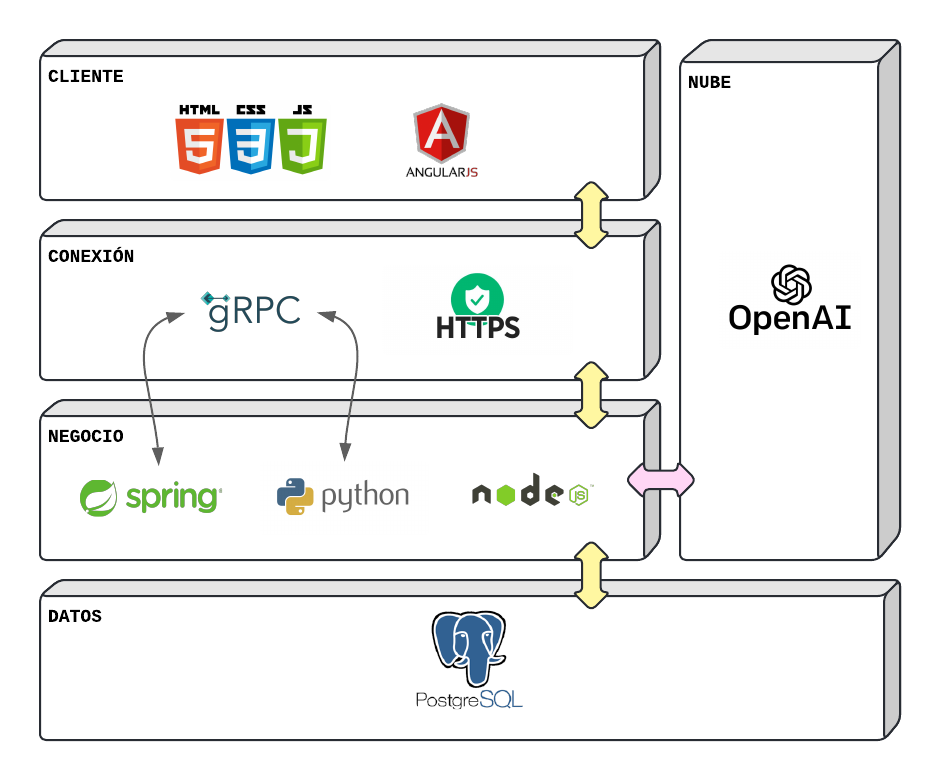
\includegraphics[width=\textwidth]{cap3_arquitectura.png}
	\caption{Arquitectura de la extensión.}
	\label{fig:cap3_arquitectura}
\end{figure}


\subsection{Capa del Cliente}

La capa del cliente es la interfaz donde los usuarios interactúan directamente con la herramienta y la extensión implementada. Esta capa se encarga de proporcionar una experiencia de usuario intuitiva y accesible mediante interfaces web. Los usuarios pueden acceder a las funcionalidades de la herramienta, como la creación y análisis de casos de uso, y visualizar los diagramas de clases generados. Esta capa incluye todas las vistas y componentes de la interfaz de usuario que permiten a los ingenieros de software realizar sus tareas de manera eficiente.

\begin{itemize}
	\item \textbf{Interfaces Web:} Desarrolladas utilizando tecnologías como HTML, CSS y JavaScript, junto con frameworks modernos como React o Angular, estas interfaces permiten a los usuarios interactuar con las funcionalidades de la herramienta.
	\item \textbf{Interacción Usuario-Sistema:} Los usuarios pueden enviar descripciones de casos de uso, recibir resultados del análisis y gestionar sus proyectos directamente desde el navegador web.
\end{itemize}

\subsection{Capa de Conexión}

La capa de conexión se encarga de manejar las comunicaciones entre los diferentes componentes del sistema. Esta capa es crucial para garantizar que los datos fluyan de manera eficiente y segura entre las diferentes partes del sistema.

\begin{itemize}
	\item \textbf{Conexión HTTP:} Utilizada para la comunicación entre el cliente y los microservicios backend. Las peticiones HTTP son manejadas por el framework Spring, que gestiona la validación de las solicitudes y la entrega de respuestas adecuadas.
	\item \textbf{Conexión gRPC:} Establecida entre los microservicios de Spring y el componente de Python que maneja la integración con los modelos de inteligencia artificial. gRPC proporciona una comunicación rápida y eficiente, esencial para el procesamiento intensivo de datos requerido por los modelos de IA.
\end{itemize}

\subsection{Capa de Negocio}

La capa de negocio alberga todos los microservicios implementados que contienen la lógica del negocio necesaria para manejar el uso de los modelos de inteligencia artificial y el entrenamiento de los mismos. Esta capa es el núcleo funcional de la aplicación, donde se llevan a cabo las principales operaciones.

\begin{itemize}
	\item \textbf{Microservicios:} Desarrollados con Spring Boot, estos servicios incluyen funcionalidades como la gestión de usuarios, el procesamiento de descripciones de casos de uso, y la generación de diagramas de clases.
	\item \textbf{Lógica de Negocio:} Cada microservicio está diseñado para realizar tareas específicas, como la validación de peticiones, el análisis de texto utilizando modelos de IA, y la generación y refinamiento de diagramas de clases conceptuales.
\end{itemize}

\subsection{Capa de la Nube}

La capa de la nube se refiere al uso de servicios externos, en este caso, los modelos de OpenAI. Esta capa proporciona las capacidades de inteligencia artificial necesarias para analizar las descripciones de los casos de uso y generar estructuras JSON que representen diagramas de clases.

\begin{itemize}
	\item \textbf{Modelos de IA:} Utilización de modelos de inteligencia artificial para procesar texto y extraer información relevante. Los modelos pueden ser seleccionados y configurados según las necesidades del desarrollador.
	\item \textbf{API de OpenAI:} La integración con la API de OpenAI permite el acceso a potentes modelos de IA que facilitan el análisis y procesamiento de las descripciones textuales, optimizando el proceso de diseño de sistemas.
\end{itemize}

\subsection{Capa de Datos}

La capa de datos es responsable de almacenar toda la información relevante generada y utilizada por el sistema. Esto incluye los modelos y entrenamientos realizados, así como los diagramas de clases generados a partir de los análisis.

\begin{itemize}
	\item \textbf{Base de Datos PostgreSQL:} Utilizada para almacenar descripciones textuales, estructuras JSON generadas, diagramas de clases y cualquier otro dato relevante. PostgreSQL es una base de datos relacional robusta y escalable, adecuada para aplicaciones de misión crítica.
	\item \textbf{Almacenamiento de Modelos:} Los datos relacionados con los modelos de IA, incluyendo los resultados del entrenamiento y las configuraciones utilizadas, son almacenados de manera segura para asegurar su disponibilidad y fácil acceso cuando sea necesario.
\end{itemize}

\section{Desarrollo e Implementación}

El desarrollo e implementación de la extensión de la herramienta TDDT4IoTS se llevó a cabo a través de una serie de fases bien definidas, cada una de las cuales fue importante para cumplir con el objetivo principal del proyecto. Este enfoque estructurado permitió un desarrollo iterativo, asegurando que cada componente del sistema fuera desarrollado y probado de manera correcta antes de proceder a la siguiente fase. El proceso comenzó con un análisis detallado de los requisitos, seguido por el diseño de la extensión, la configuración de los frameworks necesarios, el desarrollo de los componentes y, finalmente, la integración de estos componentes en un sistema funcional.

En la figura \ref{fig:cap3_fases_desarrollo} se observa cada fase del desarrollo se llevó a cabo con un enfoque metodológico que incluyó la planificación, la implementación y la revisión constante para asegurar la calidad del sistema final. En la primera fase, se realizó un análisis de los requisitos para definir las funcionalidades y características necesarias. En la segunda fase, se diseñaron los componentes de la extensión basándose en los requisitos definidos. La tercera fase implicó la configuración de los frameworks y herramientas que soportarían el desarrollo, mientras que en la cuarta fase se desarrollaron los componentes individuales. Finalmente, en la quinta fase, se llevó a cabo la integración de todos los componentes desarrollados, asegurando que funcionaran conjuntamente.

\begin{figure}[H]  
	\centering
	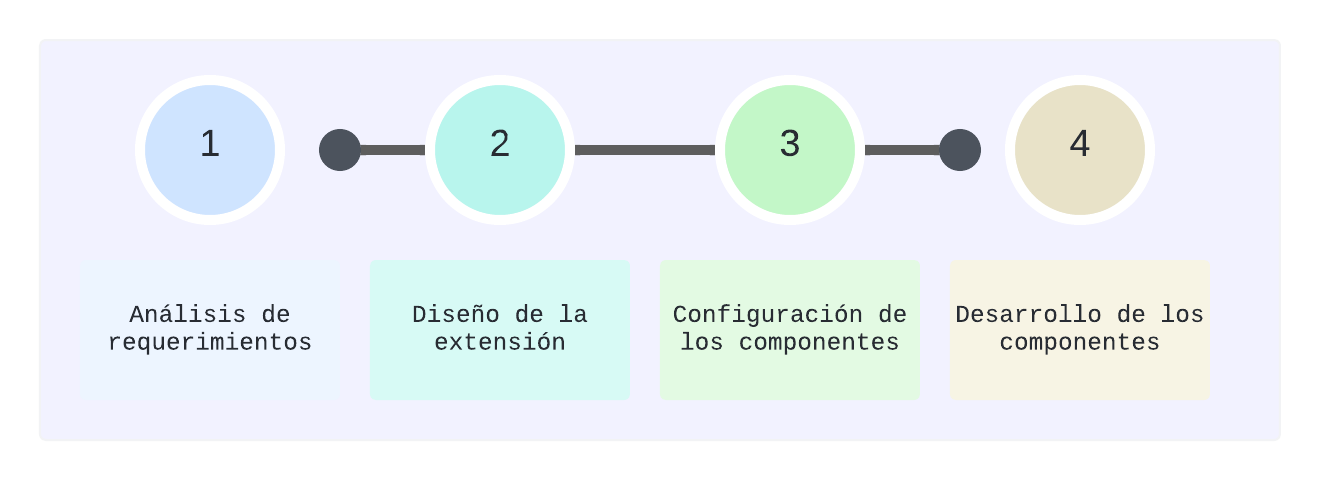
\includegraphics[width=\textwidth]{cap3_fases_desarrollo.png}
	\caption{Fases de Desarrollo.}
	\label{fig:cap3_fases_desarrollo}
\end{figure}


\subsection{Fase 1: Análisis de requerimientos}

Para llevar a cabo la ejecución correcta de los requisitos funcionales de la extensión, fue necesario utiliza una serie de tecnologías útiles para cumplir con el objetivo principal del trabajo. A continuación se detallan las tecnologías y software utilizados para el desarrollo e implementación del proyecto.

\subsubsection{Tecnologías}

\textbf{Capa del cliente}

\begin{itemize}
	\item \textbf{AngularJs:} Para mantener el correcto funcionamiento de la herramienta TDDT4IOTS, se decidió continuar utilizando esta librería para generar las nuevas interfaces web. Esto permite que los usuarios sigan utilizando la herramienta de la misma manera que lo hacían anteriormente.
\end{itemize}

\textbf{Capa de conexión}

\begin{itemize}
	\item \textbf{gRPC:} Este protocolo de comunicación facilita la integración interna de componentes en el servidor. Su objetivo es aprovechar las ventajas de diversas tecnologías y permitir que trabajen conjuntamente, asignando cargas de trabajo que pueden ser mejor ejecutadas por otras tecnologías.
	
	\item \textbf{HTTP:} Es uno de los protocolos más utilizados por aplicaciones web. Permite enviar y recibir datos entre un navegador web y el servidor, lo que es esencial para cumplir con los objetivos de cualquier proyecto implementado. En la extensión de la herramienta, permite realizar las peticiones necesarias al servidor y obtener respuestas con datos limpios que se mostrarán al usuario.
	
\end{itemize}

\textbf{Capa de negocio}

\begin{itemize}
	\item \textbf{Spring Framework:} Para procesar todas las peticiones de la extensión, se utilizó el framework Spring, que emplea Java como lenguaje de programación. Java es conocido por su robustez y su capacidad para manejar un alto volumen de solicitudes. Considerando la cantidad de peticiones que se recibirán cuando se utilice la extensión mediante la herramienta, se busca mantener una conexión estable y aprovechar todas las ventajas que ofrece Spring Framework. Este framework es ideal para este proceso debido a su capacidad para manejar concurrencia, su soporte para transacciones, y su eficiente gestión de recursos. Además, Spring Framework permite ofrecer respuestas rápidas a las peticiones, gracias a su alta capacidad de procesamiento de datos y a su arquitectura modular, que facilita el mantenimiento y la escalabilidad de la aplicación.
	
	\item \textbf{NodeJs:} La herramienta cuenta con un intérprete que analiza la redacción de los casos de uso creados mediante la misma. Este intérprete, denominado ArmadilloJs, fue desarrollado como una librería JavaScript que puede ser implementada incluyendo el script en un documento HTML y utilizar sus funciones. Para generar los archivos necesarios para el entrenamiento de los modelos de OpenAI, surgió la necesidad de migrar la librería a un servicio web. Dado que la librería fue programada en JavaScript, se decidió implementar el servicio web con Node.js. Esta elección permite utilizar el intérprete de forma interna a través de los microservicios proporcionados por Spring Framework, aprovechando la compatibilidad y eficiencia de Node.js para manejar solicitudes asíncronas y el robusto manejo de transacciones y recursos de Spring Framework.
	
	\item \textbf{Python:} Como parte de la extension, se hace uso de la API de OpenAI. Python se destaca como uno de los lenguajes más utilizados en tecnologías de inteligencia artificial debido a su simplicidad, versatilidad y una amplia gama de bibliotecas especializadas. Aprovechando la existencia de una biblioteca de OpenAI para Python, se implementó la comunicación con OpenAI para mantener una interacción más fluida y bien desarrollada. Además, Python ofrece ventajas significativas en el desarrollo de aplicaciones de IA, como una sintaxis clara y legible, una gran comunidad de desarrolladores y soporte extensivo para frameworks y herramientas de aprendizaje automático y procesamiento de datos. Estas características hacen de Python la elección ideal para integrar OpenAI y aprovechar al máximo sus capacidades de IA en la herramienta.
	
\end{itemize}

\textbf{Capa de la nube}

\begin{itemize}
	\item \textbf{OpenAI:} La comunicación con la API de OpenAI permite utilizar los recursos almacenados en sus servidores. Esto da una ventaja de no utilizar recursos locales para implementar modelos de inteligencia artificial desde cero. También aprovechando los recursos de OpenAI se almacenan los datos entrenados por cada cuenta de usuario que este registrada en sus servicios. Cabe recalcar que también se almacena ciertos datos de forma local. 
\end{itemize}

\textbf{Capa de datos}

\begin{itemize}
	\item \textbf{PostgreSQL:} La comunicación con la API de OpenAI permite utilizar los recursos alojados en sus servidores, lo cual ofrece la ventaja de no necesitar recursos locales para implementar modelos de inteligencia artificial desde cero. Al aprovechar los recursos de OpenAI, los datos entrenados se almacenan por cuenta de usuario registrada en sus servicios. Además, es importante destacar que algunos datos también se almacenan localmente para mejorar la eficiencia y disponibilidad. Esta combinación de almacenamiento en la nube y local asegura un rendimiento óptimo y una gestión eficiente de los datos.
\end{itemize}


\subsubsection{Software}

Durante el desarrollo de nuestro proyecto, se utilizaron diversas herramientas de software proporcionadas por JetBrains para maximizar la eficiencia y productividad. JetBrains ofrece un conjunto robusto de entornos de desarrollo integrado (IDE) que se adaptan a diversas necesidades y lenguajes de programación. Entre las herramientas empleadas se encuentran IntelliJ IDEA, que proporcionó un potente soporte para el desarrollo en Java; WebStorm, que facilitó la creación de aplicaciones web con tecnologías como JavaScript y TypeScript; PyCharm, que optimizó el desarrollo en Python, especialmente para aplicaciones de inteligencia artificial y análisis de datos; y DataGrip, que mejoró significativamente la gestión y el análisis de bases de datos. El uso de estas herramientas avanzadas nos permitió abordar diversas fases del desarrollo con mayor eficiencia y precisión.

\textbf{IntelliJ IDEA 2024.1.4}

Para el desarrollo en Java, utilizamos \textbf{IntelliJ IDEA 2024.1.4}, que proporcionó un entorno robusto y eficiente. Este IDE fue fundamental para la integración de Spring Framework y la gestión de microservicios, permitiéndonos escribir, probar y depurar código de manera efectiva. Las características avanzadas de IntelliJ, como la autocompletación inteligente, el análisis de código en tiempo real y las herramientas de refactorización, mejoraron significativamente nuestra productividad y calidad del código.

\textbf{WebStorm 2023.3.1}

En el desarrollo de interfaces web, \textbf{WebStorm 2023.3.1} fue la herramienta elegida por su capacidad para manejar tecnologías modernas como AngularJS. WebStorm facilitó la creación de interfaces web responsivas y dinámicas, proporcionando un entorno de desarrollo con soporte completo para JavaScript, TypeScript, HTML y CSS. Las capacidades de depuración en vivo y las herramientas de desarrollo front-end de WebStorm nos permitieron iterar rápidamente y mantener un alto estándar de calidad en nuestras interfaces de usuario.

\textbf{PyCharm 2023.3.4}

Para los scripts en Python que gestionan la comunicación con la API de OpenAI, utilizamos \textbf{PyCharm 2023.3.4}. Este IDE es reconocido por su excelente soporte para el desarrollo en Python, especialmente en proyectos de inteligencia artificial y análisis de datos. PyCharm proporcionó herramientas integradas para la gestión de entornos virtuales, el análisis de código y la depuración, lo que facilitó la implementación de soluciones robustas y eficientes para la comunicación con OpenAI.

\textbf{DataGrip 2023.2.3}

La gestión de bases de datos fue mejorada significativamente mediante el uso de \textbf{DataGrip 2023.2.3}. Esta herramienta nos permitió realizar un análisis eficiente y una integración perfecta con los demás componentes del sistema. DataGrip soporta múltiples sistemas de gestión de bases de datos, ofreciendo características avanzadas como la navegación por esquemas, la edición inteligente de SQL y la visualización de datos, lo que mejoró nuestra capacidad para gestionar y manipular grandes volúmenes de datos de manera efectiva.

\textbf{NetBeans 22}

En ciertos desarrollos específicos, utilizamos \textbf{NetBeans 22}, un IDE versátil que soporta múltiples lenguajes de programación. NetBeans facilitó el desarrollo de aplicaciones modulares y permitió una integración sencilla con diversas herramientas de desarrollo. Su interfaz intuitiva y sus poderosas características de depuración y gestión de proyectos lo hicieron una opción adecuada para tareas específicas dentro del proyecto.

\textbf{Postman}

Para probar y depurar las API, \textbf{Postman} fue una herramienta esencial. Postman nos permitió realizar solicitudes HTTP de manera eficiente, probar los endpoints del servidor y validar las respuestas. Su interfaz amigable y sus capacidades avanzadas de testing automatizado nos ayudaron a asegurar que todas las comunicaciones entre los componentes del sistema fueran precisas y confiables.


\subsection{Fase 2: Diseño de la extensión}

En esta fase se explicará detalladamente el comportamiento de cada proceso necesario para que la extensión de la herramienta funcione correctamente. Se dedicó tiempo a analizar cuál sería la mejor forma de adaptar la nueva funcionalidad a la herramienta sin afectar los componentes existentes.

\textbf{Modelos}

OpenAI ofrece una variedad de modelos que pueden ser utilizados mediante el ajuste fino. Esta técnica permite entrenar modelos para especializarlos en tareas específicas, adaptándolos a las necesidades particulares del proyecto en el que se esté trabajando. Se llegó a la conclusión de registrar los posibles modelos base dentro de la herramienta, lo que permite seleccionar el modelo base adecuado para iniciar un nuevo entrenamiento y ponerlo a disposición de todos los usuarios.

Además, el proceso de ajuste fino no solo optimiza la precisión del modelo, sino que también mejora su eficiencia en la tarea específica, reduciendo el tiempo y los recursos necesarios para obtener resultados precisos. De esta manera, OpenAI asegura que sus usuarios puedan aprovechar al máximo las capacidades avanzadas de sus modelos de inteligencia artificial, facilitando la implementación de soluciones innovadoras y efectivas en diversos ámbitos.

\textbf{Entrenar modelos}

El ajuste fino permitió entrenar modelos existentes para cumplir con los requisitos funcionales del proyecto. Cada entrenamiento será registrado dentro de la herramienta, permitiendo llevar un historial detallado de todos los entrenamientos realizados a los modelos seleccionados. Esta tarea será llevada a cabo por los usuarios interesados en entrenar modelos. Para entrenar modelos, se debe seguir una serie de pasos que se han tratado de automatizar por completo. Es necesario contar con una secret key de OpenAI para poder entrenar estos modelos. Además, se necesita un conjunto de datos que serán enviados al modelo mediante el ajuste fino y esperar los resultados del entrenamiento.

El archivo debe contener las posibles peticiones y respuestas que el modelo debe procesar cuando sea utilizado por otros usuarios mediante la herramienta. Este archivo actúa como una guía de comportamiento, asegurando que el modelo responda adecuadamente a diferentes escenarios. Además, es crucial que los datos estén bien estructurados y sean representativos de los casos de uso reales para garantizar la eficacia del entrenamiento. De esta manera, se optimiza el rendimiento del modelo y se mejora la precisión de sus respuestas, facilitando su integración y uso en aplicaciones prácticas.

\textbf{Uso de modelos}

Teniendo algunos modelos entrenados, se puede hacer uso de ellos para interpretar las descripciones de los casos de uso redactados en lenguaje natural. El usuario interesado en el entrenamiento realizado por otro usuario podrá seleccionarlo desde el historial de entrenamiento. Para llevar a cabo este proceso, también se debe contar con una secret key para poder acceder al modelo entrenado. Debido a que OpenAI solo permite acceder al modelo entrenado con la misma secret key con la que fue entrenado, se implementó la funcionalidad de compartir la secret key del usuario que entrenó el modelo para facilitar el acceso sin problemas.

\subsection{Fase 3: Configuración de los componentes}

En la siguiente fase se detallan los componentes que fueron configurados para abarcar la funcionalidad completa de la extensión. Cada componente está diseñado para cumplir con una funcionalidad específica, asegurando que el sistema no solo cumpla con los requisitos actuales, sino que también sea escalable y mantenible a lo largo del tiempo. Se han tomado en cuenta prácticas de diseño modular y principios de ingeniería de software que permiten una fácil actualización y expansión de la herramienta, facilitando así su adaptación a futuras necesidades y mejoras tecnológicas.

\begin{itemize}
	\item \textbf{db-repository-tddt4iots: } Para mantener la conexión a la base de datos del proyecto, se configuró este componente como una dependencia del proyecto principal. El objetivo de este componente es centralizar todas las operaciones relacionadas con el acceso a datos, incluyendo el mapeo de entidades de la base de datos a clases Java, la ejecución de consultas SQL, y otras tareas de manejo de datos. Esta configuración permite una gestión más eficiente y organizada de las interacciones con la base de datos, asegurando un acceso a datos consistente y fiable.
	
	\item \textbf{ms-core-tddt4iots: } Este componente se encargará de contener todos los DTO necesarios para realizar las peticiones y respuestas, tanto del cliente al servidor como del servidor a la base de datos. Además, incluirá métodos utilitarios que podrán ser utilizados por otros componentes o proyectos generales, facilitando la reutilización de código y mejorando la eficiencia del desarrollo.
	
	\item \textbf{ms-core-tddt4iots-openai} Este componente constituye el proyecto principal y utiliza como dependencias los demás proyectos mencionados anteriormente. En este proyecto se configurarán todos los microservicios que se liberarán y que podrán ser consumidos por la extensión, asegurando así una integración fluida y coherente. Además, este proyecto se encarga de configurar los parámetros necesarios para acceder a la base de datos, manteniendo los objetos de datos aislados en sus respectivas dependencias. Esta separación de responsabilidades no solo mejora la organización del código, sino que también facilita el mantenimiento y la escalabilidad del sistema. Al centralizar la configuración de los microservicios y las conexiones a la base de datos, este componente principal actúa como el núcleo del sistema, permitiendo una gestión eficiente de las interacciones entre los diferentes módulos y garantizando que todas las partes del proyecto funcionen de manera cohesiva y eficiente. 
	
	\item \textbf{ms\_core\_tddt4iots\_py: } Para implementar el uso del lenguaje de programación Python, se configuró este proyecto como un servidor gRPC. Este componente facilita la comunicación eficiente y rápida con la API de OpenAI mediante las librerías correspondientes, permitiendo tanto el entrenamiento como el uso de los modelos existentes. Dentro de este proyecto, se gestionan todas las interacciones con OpenAI, asegurando que las solicitudes y respuestas sean manejadas de manera óptima. La configuración del servidor gRPC permite una comunicación robusta y de baja latencia entre los diferentes servicios y el backend de OpenAI, lo que es crucial para operaciones que requieren procesamiento en tiempo real. Además, este proyecto no solo se limita a gestionar el entrenamiento de los modelos, sino que también supervisa su implementación y actualización continua. Al utilizar gRPC, se garantiza que las conexiones sean seguras y eficientes, facilitando el desarrollo y la integración de nuevas funcionalidades basadas en inteligencia artificial.
	
	\item \textbf{armadillo-api: } La herramienta originalmente incluía un intérprete de descripciones de casos de uso redactadas en un lenguaje de símbolos. Este componente se configuró como un servicio web, permitiendo su utilización a través de una API REST que integra la biblioteca de JavaScript correspondiente. Esta configuración facilita el acceso y la interpretación de los casos de uso, asegurando que las descripciones sean procesadas de manera eficiente y precisa. Además, la implementación como servicio web permite una mayor flexibilidad y escalabilidad, permitiendo que otros sistemas y aplicaciones puedan interactuar con el intérprete de manera sencilla y consistente.

\end{itemize}

\subsection{Fase 4: Desarrollo de los componentes}

En esta fase se detalla todo lo desarrollado dentro de cada componente. Durante el desarrollo de esta fase, se logró aclarar y abordar todos los requisitos funcionales mencionados en la documentación del proyecto. A continuación, se describirán los paquetes implementados en cada componente y los pasos que se definieron para llevar a cabo la interpretacion de los casos de uso redactados en lenguaje natural para asegurar el funcionamiento completo de la extensión en la herramienta y satisfacer las necesidades del usuario final.

\begin{itemize}
	\item \textbf{db-repository-tddt4iots: } Dentro de este componente se empezó con el desarrollo de todos los paquetes necesarios para estructurar todos los objetos que intervienen en el manejo de los datos. En el paquete \texttt{config} se detalló la configuración de los repositorios y transacciones JPA para la extensión de la herramienta. El paquete \texttt{entity} es donde se crearon todas las entidades mapeando las tablas de la base de datos. \texttt{repository} contiene todas las sentencias \texttt{SQL} que permitirán obtener los datos para las entidades. Finalmente, el paquete \texttt{impl} contendrá todas las implementaciones de las interfaces del paquete \texttt{service} para liberar los métodos existentes al proyecto que esté utilizando este componente como dependencia (ver figura \ref{fig:cap3_comp_db_pack}).
	
	\begin{figure}[H]
		\centering
		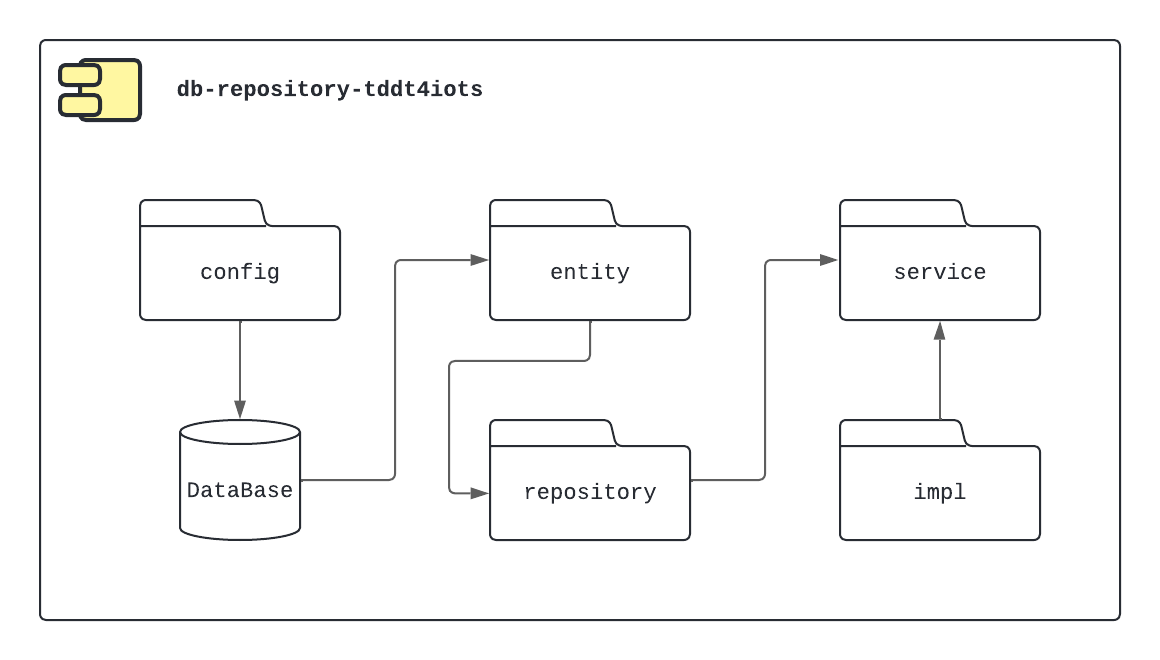
\includegraphics[width=\textwidth]{cap3_comp_db_pack.png}
		\caption{Paquetes desarrollados dentro del componente db-repository-tddt4iots.}
		\label{fig:cap3_comp_db_pack}
	\end{figure}
	
	\item \textbf{ms-core-tddt4iots: } Se estructura en varios paquetes, cada uno con objetivos específicos: el paquete \texttt{config} gestiona la configuración necesaria para la comunicación gRPC y puede ser escalable para desarrollar otras clases que permitan la conexión con otros tipos de protocolos; \texttt{cons} almacena constantes utilizadas en todo el proyecto; \texttt{util} contiene utilidades y funciones auxiliares reutilizables; \texttt{proto} incluye los archivos \texttt{.proto} que definen los métodos y mensajes gRPC para la interacción entre componentes; \texttt{dto} alberga los Data Transfer Objects, organizados en \texttt{request} para solicitudes y \texttt{response} para respuestas; y finalmente, \texttt{grpc\_service} contiene las implementaciones de los servicios gRPC definidos en los archivos .proto, asegurando una integración eficiente y consistente en todo el proyecto (ver figura \ref{fig:cap3_comp_core_pack}).
	
	\begin{figure}[H]
		\centering
		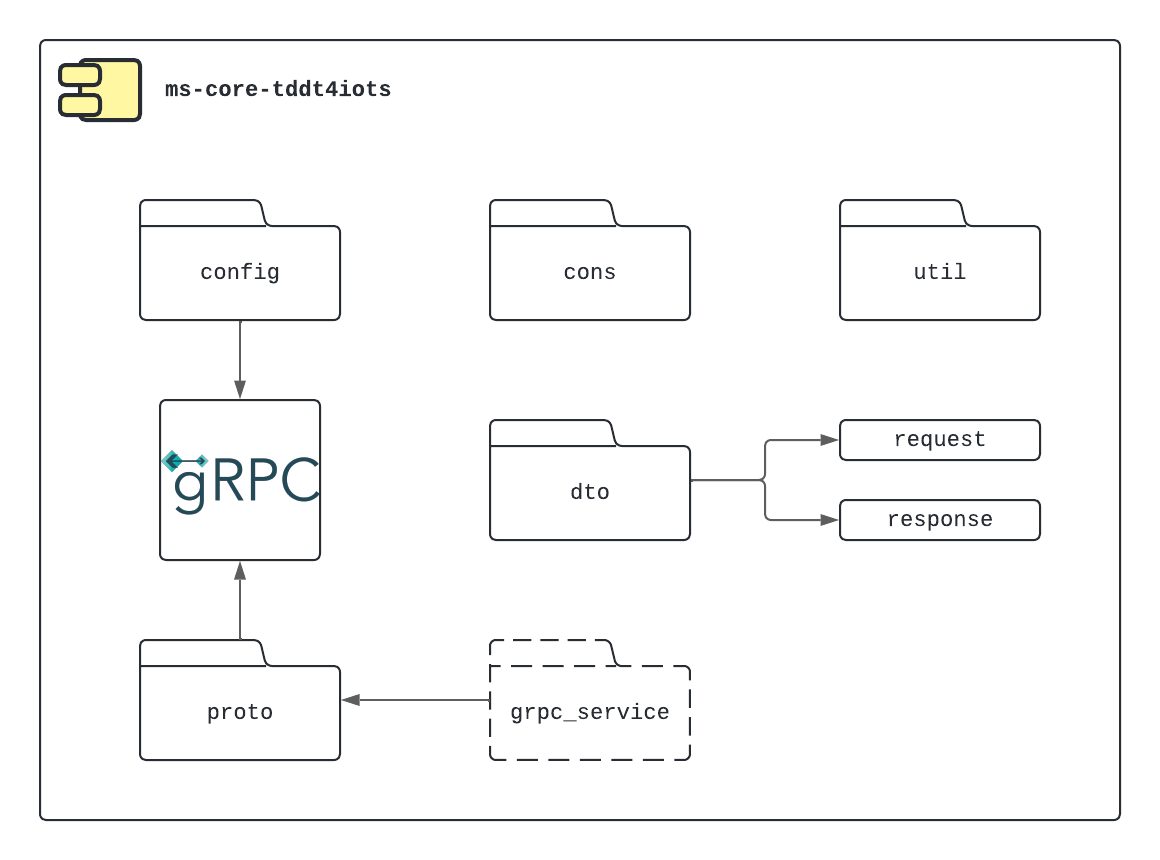
\includegraphics[width=\textwidth]{cap3_comp_core_pack.png}
		\caption{Paquetes desarrollados dentro del componente ms-core-tddt4iots.}
		\label{fig:cap3_comp_core_pack}
	\end{figure}
	
	\item \textbf{ms-core-tddt4iots-openai: } El paquete \texttt{config} gestiona la configuración necesaria para el funcionamiento del proyecto, configura el uso de las propiedades declaras en en el archivo \texttt{application.properties} y también incluye la configuración del cliente \texttt{gRPC}. El paquete \texttt{rest} se encarga de las interfaces \texttt{REST}, permitiendo la interacción del proyecto a través de llamadas HTTP. \texttt{communication} alberga la lógica de comunicación tanto \texttt{gRPC} como \texttt{REST}, facilitando la interacción fluida entre los componentes internos y externos. El paquete bo define las clases de negocio y la lógica empresarial, encapsulando los procesos del sistema, mientras que impl contiene las implementaciones concretas de estas interfaces y servicios. \texttt{grpc} maneja las operaciones relacionadas con \texttt{gRPC}, asegurando una comunicación eficiente con el servidor de Python que utiliza la librería de OpenAI. El paquete \texttt{mapper} incluye los mapeadores necesarios para convertir entidades entre diferentes capas del sistema, y \texttt{datasource} gestiona las fuentes de datos, configurando las conexiones a la base de datos y otros servicios de almacenamiento. Este diseño permite una integración efectiva y el uso óptimo de los modelos de inteligencia artificial (ver figura \ref{fig:cap3_comp_core_openai_pack}).
	
	\begin{figure}[H]
		\centering
		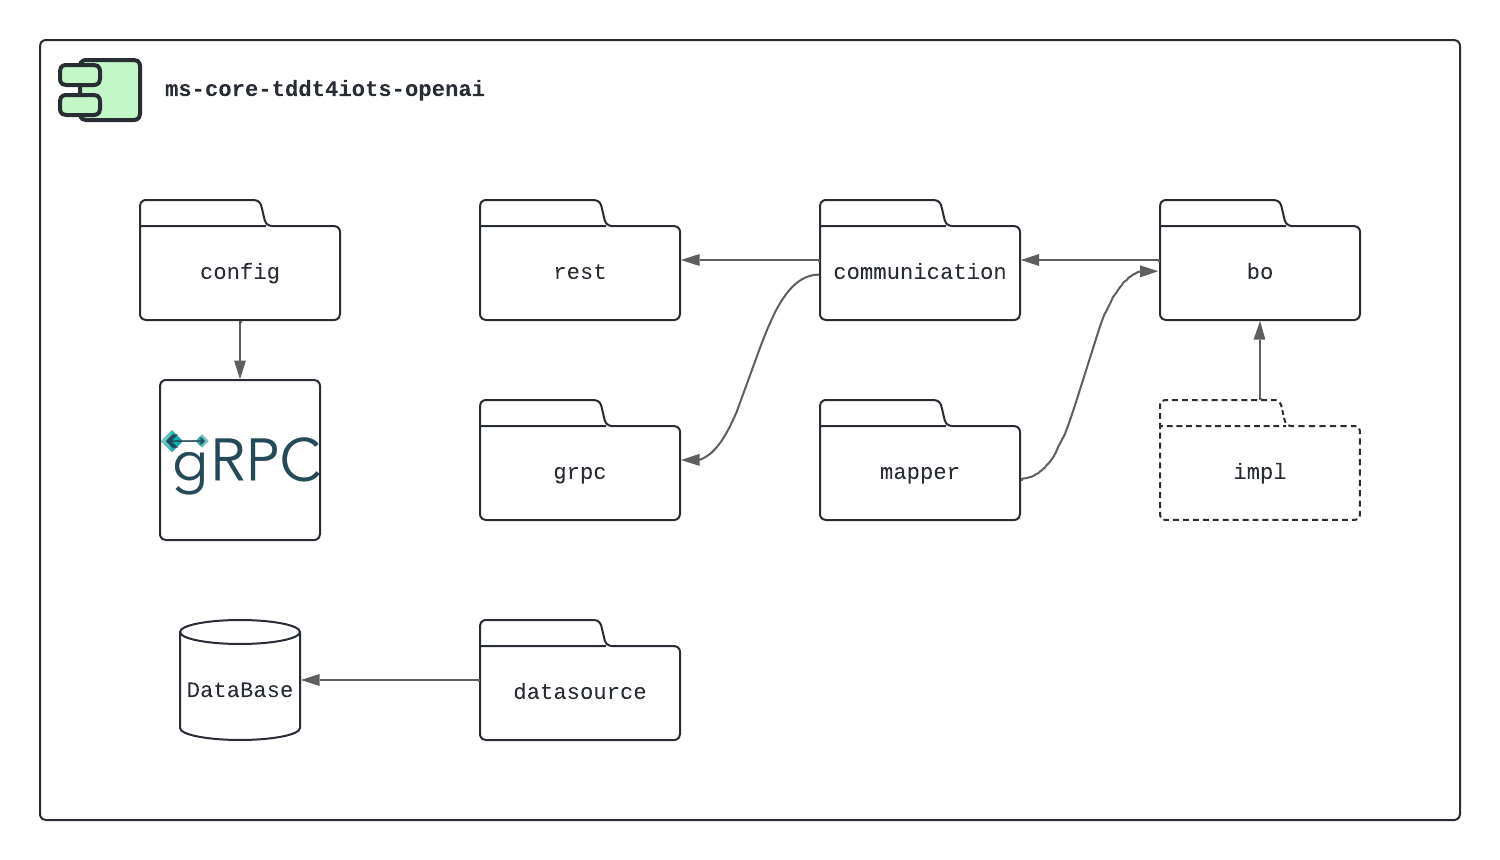
\includegraphics[width=\textwidth]{cap3_comp_core_openai_pack.png}
		\caption{Paquetes desarrollados dentro del componente ms-core-tddt4iots-openai.}
		\label{fig:cap3_comp_core_openai_pack}
	\end{figure}
	
	Dentro de este componente se detallan los tres microservicios que realizan las tareas principales del proyecto. Primero, crear los archivos en formato \texttt{JSONL} que almacenarán los \texttt{prompt}, especificando los posibles mensajes de entrada y salida que el modelo debería devolver. Segundo, entrenar el modelo; esta tarea especifica los pasos que la extensión realizará de forma interna para llevar a cabo el entrenamiento de los modelos específicos almacenados localmente. Por último, el uso de un modelo entrenado; esta tarea indicará el proceso detallado sobre cómo se recibirá la solicitud del cliente y cómo el modelo devolverá la respuesta esperada.
	
	En la figura \ref{fig:cap3_diagrama_secuencia_tarea1} se detalla el proceso analizado para la creación de los archivos JSONL y su almacenamiento, los cuales serán utilizados posteriormente en el entrenamiento de los modelos de OpenAI. Este diagrama de secuencia ilustra cada paso necesario, desde la generación de los prompts hasta su estructuración en archivos JSONL, así como la ubicación específica donde estos archivos serán almacenados. 
	
	\begin{figure}[H]  
		\centering
		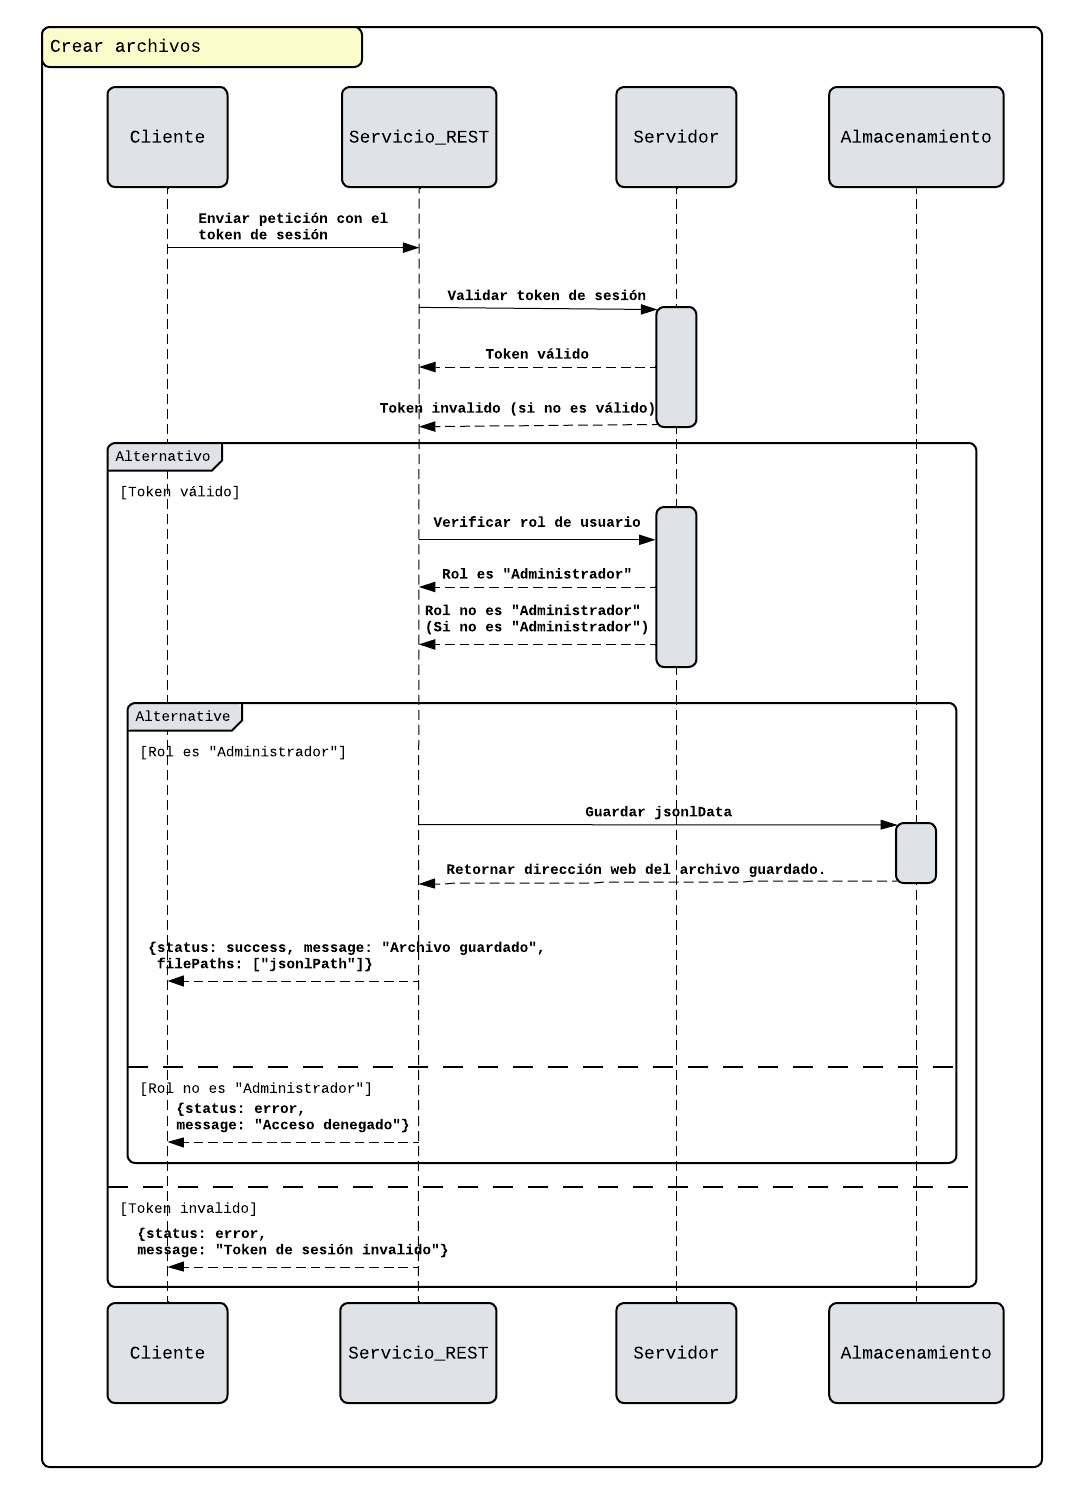
\includegraphics[width=\textwidth]{cap3_diagrama_secuencia_tarea1.png}
		\caption{Diagrama de secuencia para explicar a detalle el proceso de crear los archivos jsonl.}
		\label{fig:cap3_diagrama_secuencia_tarea1}
	\end{figure}
	
	La segunda tarea se centra en cómo se entrenará el modelo. En la figura \ref{fig:cap3_diagrama_secuencia_tarea2} ejecutará de forma automática para llevar a cabo este proceso. Este diagrama proporciona una visión clara y estructurada del flujo de acciones necesarias para el entrenamiento del modelo, asegurando que cada etapa del proceso se realice de manera correcta.
	
	\begin{figure}[H]  
		\centering
		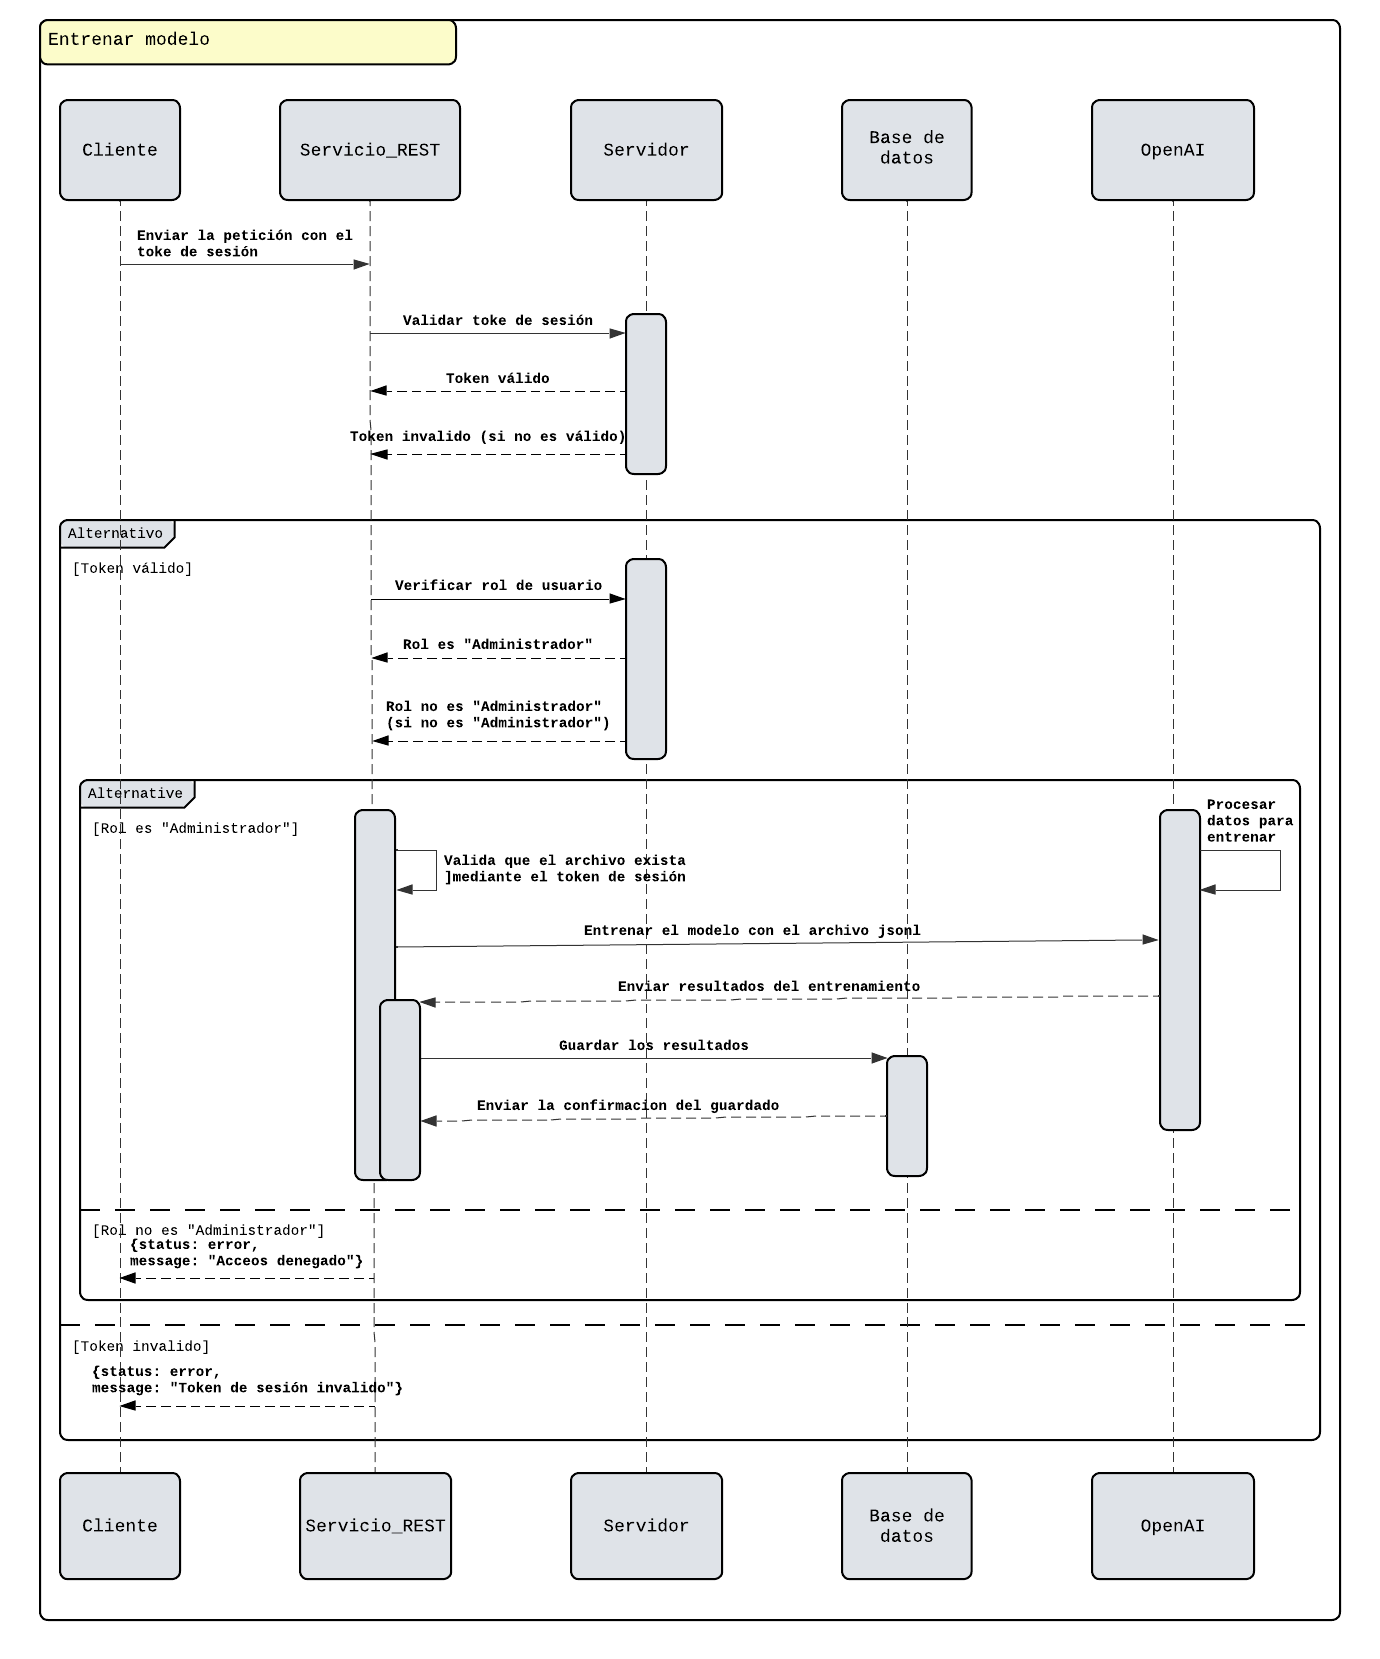
\includegraphics[width=\textwidth]{cap3_diagrama_secuencia_tarea2.png}
		\caption{Diagrama de secuencia para explicar a detalle el proceso de entrenamiento del modelo mediante el archivo jsonl.}
		\label{fig:cap3_diagrama_secuencia_tarea2}
	\end{figure}
	
	Finalmente, la tarea de implementar o usar el modelo ya entrenado se describe en la figura \ref{fig:cap3_diagrama_secuencia_tarea3}, detallando cada paso mediante un diagrama de secuencia. Para cada petición del cliente, se verifica el token de sesión para controlar quién tiene acceso a estas funcionalidades. El token se mantiene desde el componente existente en la herramienta, realizando una petición a dicho componente para no afectar la funcionalidad actual. Una vez validados los permisos, el servidor realiza una petición a la API de OpenAI para obtener la respuesta esperada.
	
	% cap3_diagrama_secuencia_tarea3
	
	\begin{figure}[H]  
		\centering
		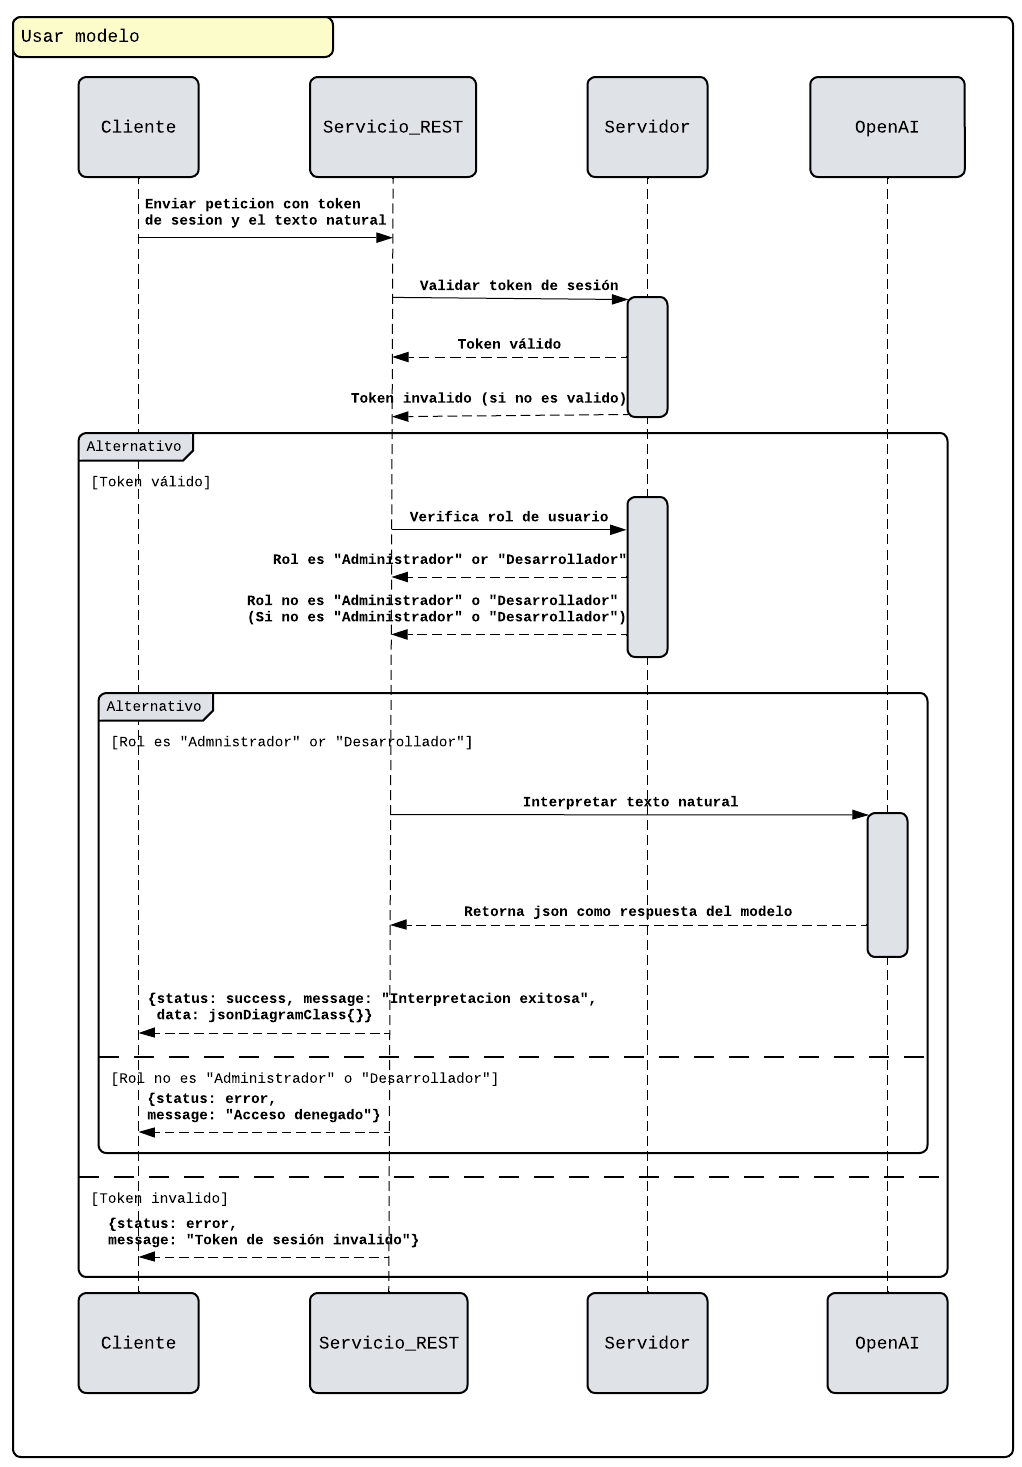
\includegraphics[width=11cm]{cap3_diagrama_secuencia_tarea3.png}
		\caption{Diagrama de secuencia para explicar a detalle el proceso de usar  el modelo.}
		\label{fig:cap3_diagrama_secuencia_tarea3}
	\end{figure}
	
	\item \textbf{ms\_core\_tddt4iots\_py: } En este componente se desarrolló el servidor gRPC para lograr la comunicación con el componente ms-core-tddt4iots-openai, con el objetivo de mantener los microservicios REST de Spring conectados con el cliente de AngularJS. Se implementaron dos métodos principales: uno para el entrenamiento del modelo y otro para su utilización, asegurando una integración eficiente y efectiva entre los distintos componentes del sistema.
		
	El paquete \texttt{proto} contiene los archivos \texttt{.proto} que definen las especificaciones de los servicios y mensajes \texttt{gRPC}, fundamentales para generar el código de comunicación. El paquete \texttt{grpc\_service} implementa estos servicios gRPC, facilitando la comunicación entre el servidor y otros componentes. El paquete \texttt{tmpFileTrain} es responsable de almacenar los archivos JSONL descargados, que son utilizados para el entrenamiento de los modelos. Por su parte, el paquete \texttt{openai\_model} alberga toda la lógica necesaria para conectarse y interactuar con la API de OpenAI, manejando las solicitudes y respuestas para integrar las funcionalidades de OpenAI en el proyecto (ver figura \ref{fig:cap3_comp_python_pack}).	
	
	\begin{figure}[H]  
		\centering
		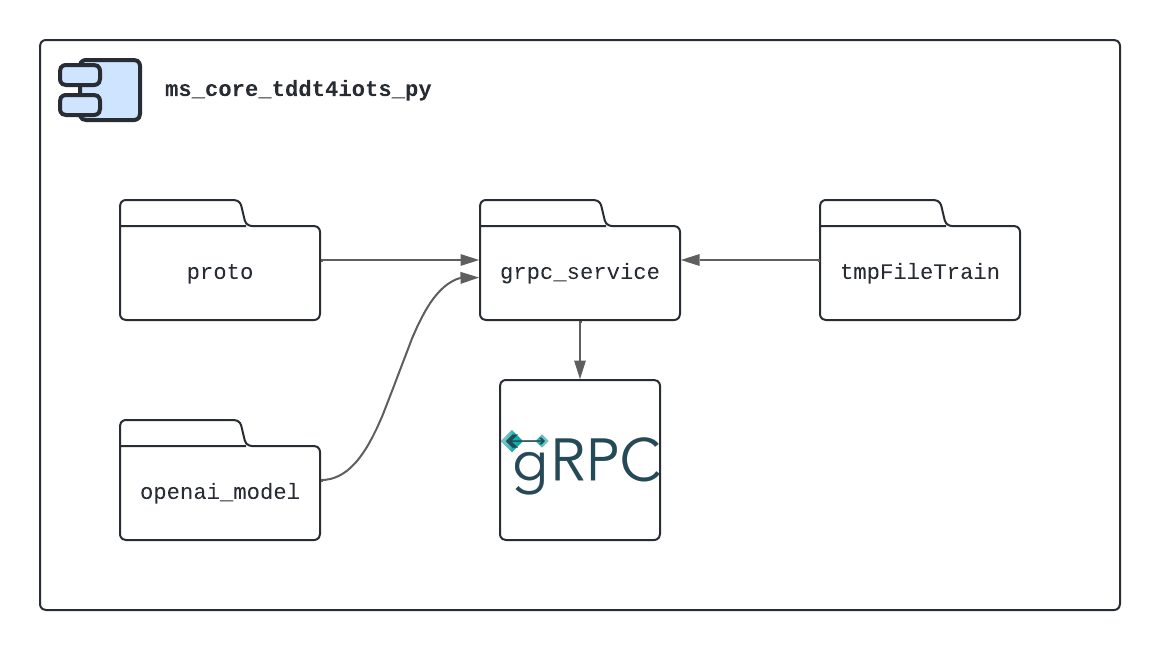
\includegraphics[width=11cm]{cap3_comp_python_pack.png}
		\caption{Paquetes desarrollados dentro del componente de python.}
		\label{fig:cap3_comp_python_pack}
	\end{figure}
	
	En la figura \ref{fig:cap3_diagrama_flujo_proceso_a} se muestra el diagrama de flujo sobre como actuar durante el entrenamiento del modelo. El método una cadena JSON con parámetros necesarios, configura el cliente de OpenAI con una clave API, descarga el archivo JSONL desde la URL especificada, y lo guarda localmente. Luego, sube este archivo a OpenAI para iniciar el proceso de fine-tuning del modelo especificado. Si el proceso se realiza con éxito, devuelve un JSON indicando el estado del entrenamiento y los detalles del fine-tuning; en caso de error, retorna un mensaje de error.

	
	\begin{figure}[H]  
		\centering
		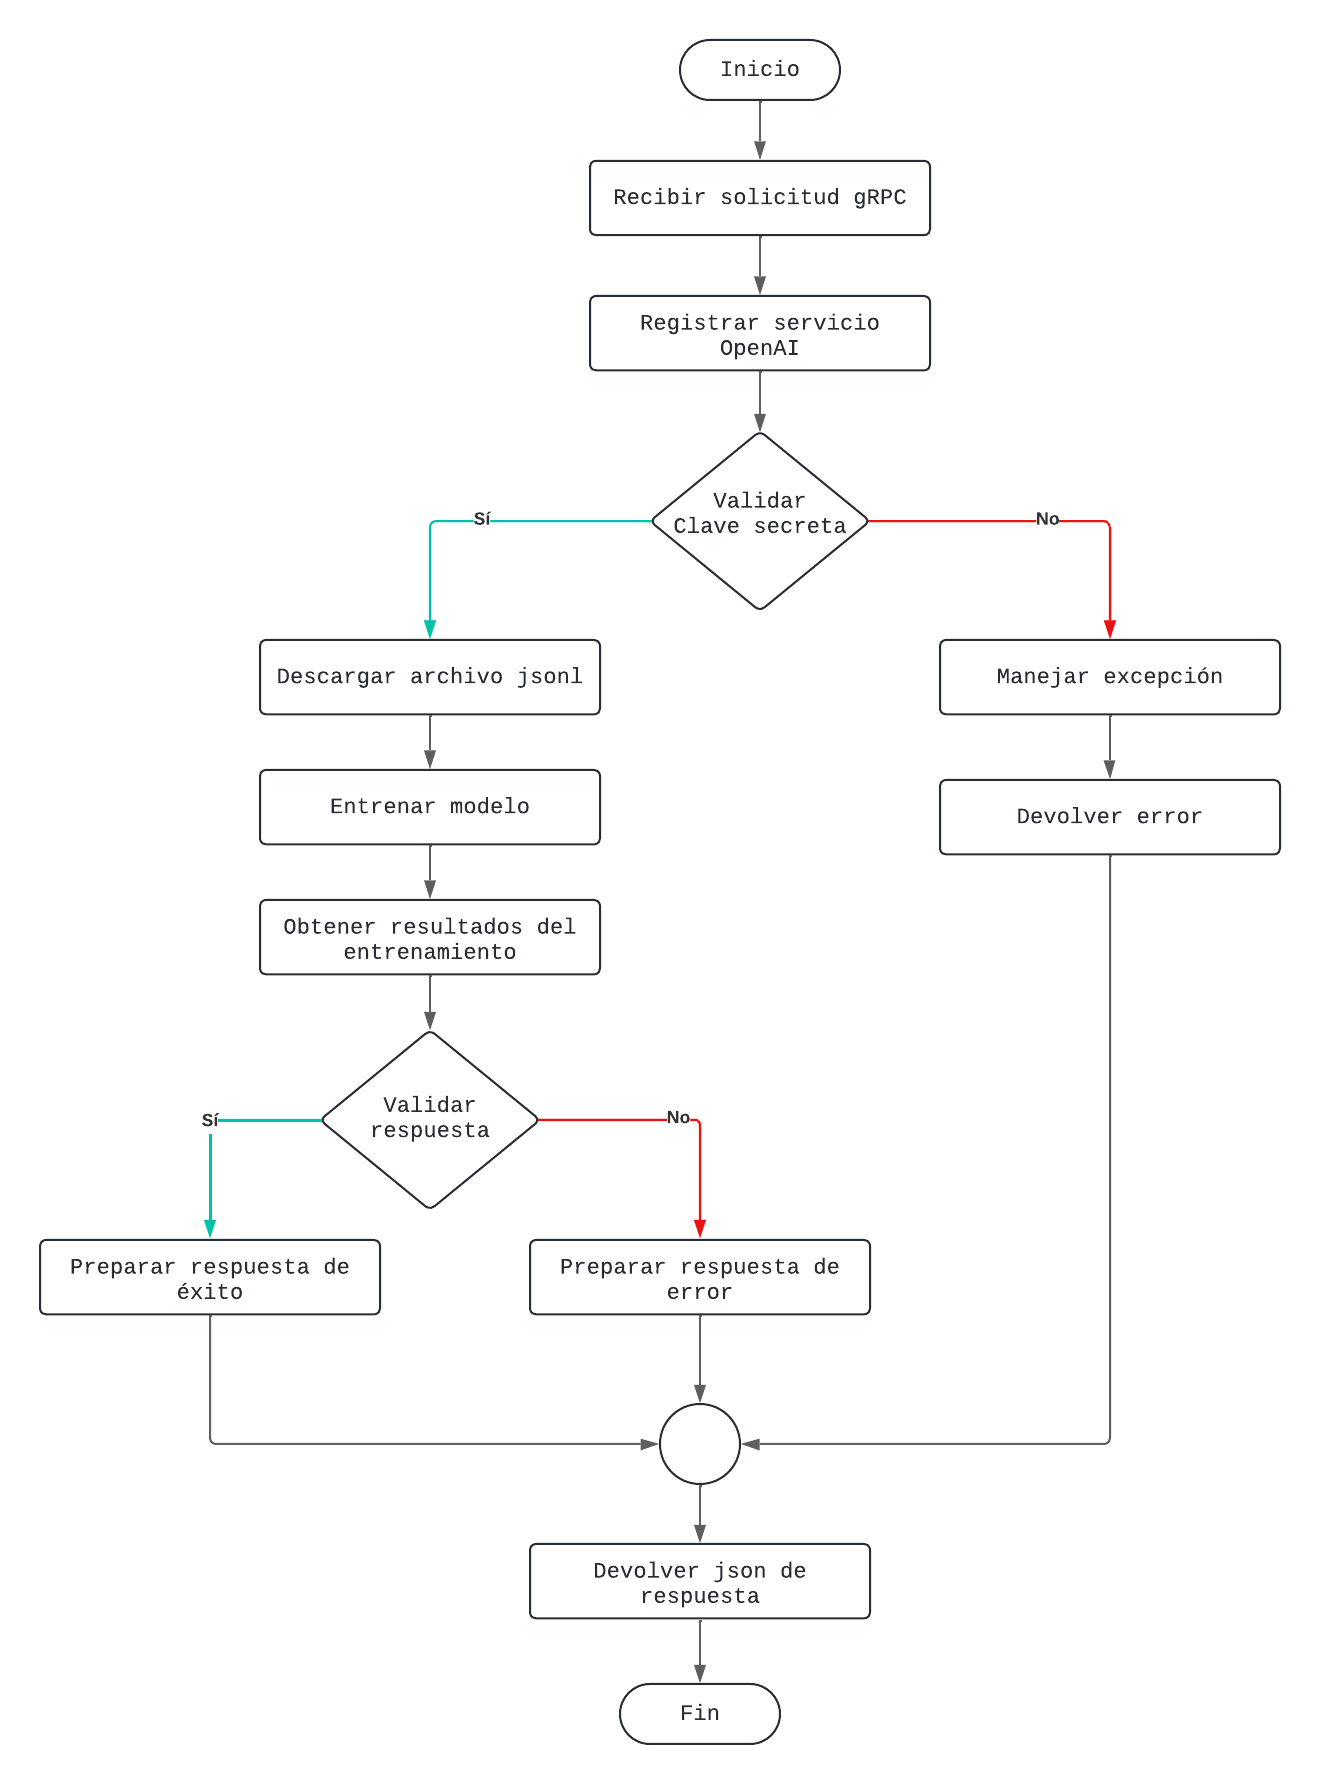
\includegraphics[width=\textwidth]{cap3_diagrama_flujo_proceso_a.png}
		\caption{Entrenamiento de los modelos de OpenAI.}
		\label{fig:cap3_diagrama_flujo_proceso_a}
	\end{figure}
	
	Para utilizar un modelo entrenado, es fundamental contar con un modelo base previamente entrenado con los datos extraídos de la herramienta. En la figura \ref{fig:cap3_diagrama_flujo_proceso_b} se muestra el proceso paso a paso que se sigue para garantizar el correcto funcionamiento de la extensión y su uso eficiente con la API de OpenAI. El proceso es muy similar al anterior con la deferencia que existe un paso denominado \texttt{Obtener mensaje promt}. Este paso contiene el texto redactado en lenguaje natural y ademas 1 mensaje en especifico detallando lo que debe realizar el modelo entrenado. 
	
	\begin{figure}[H]  
		\centering
		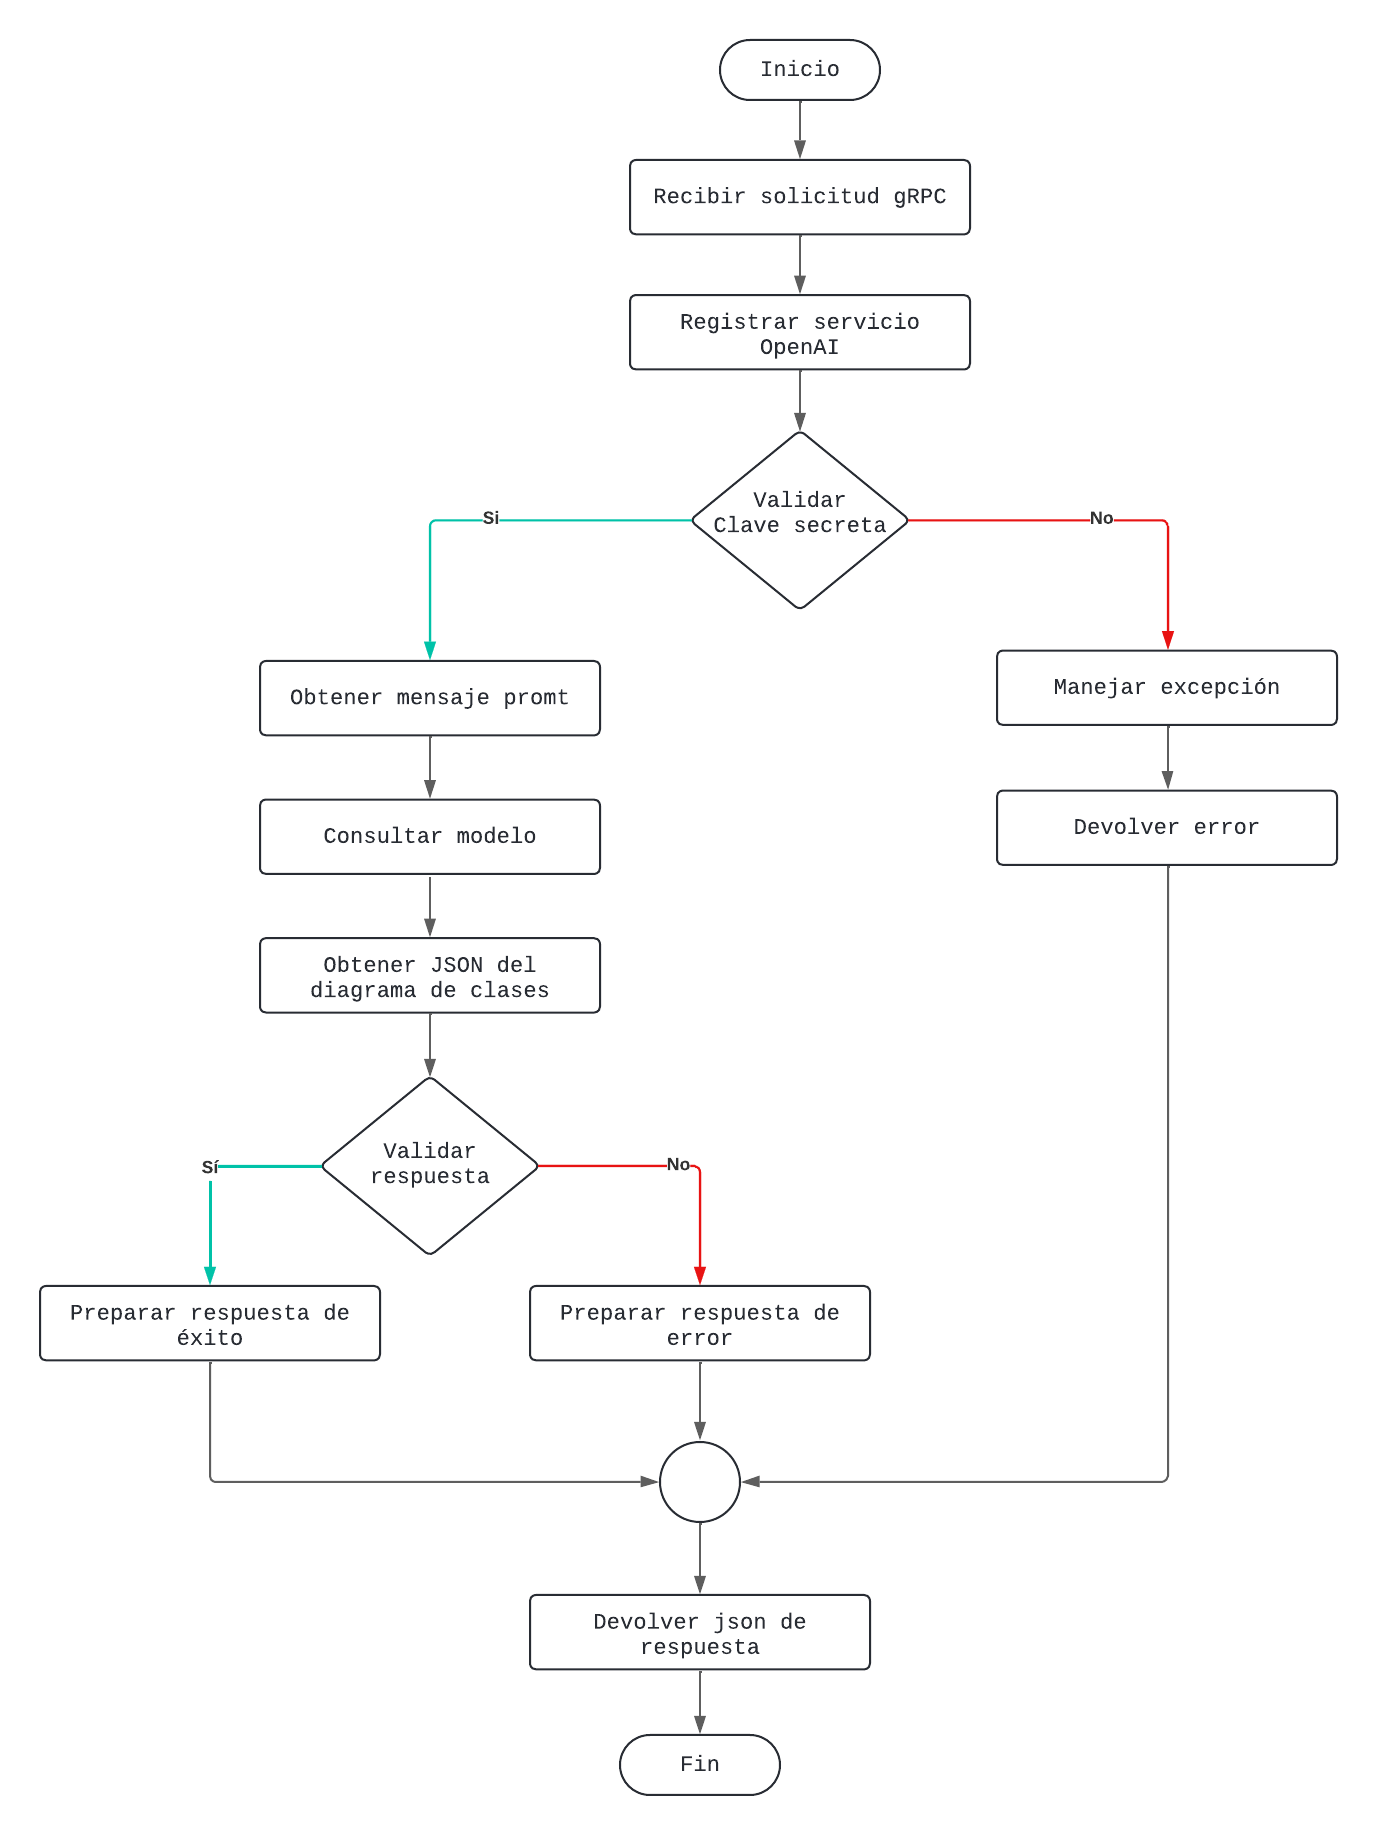
\includegraphics[width=\textwidth]{cap3_diagrama_flujo_proceso_b.png}
		\caption{Uso de los modelos entrenados por OpenAI.}
		\label{fig:cap3_diagrama_flujo_proceso_b}
	\end{figure}
	
	\item \textbf{armadillo-api: } En la herramienta actual, había un intérprete denominado ArmadilloJs que permitía convertir las descripciones de los casos de uso redactados en un conjunto de símbolos, los cuales identificaban los componentes para su diagrama de clases. Este intérprete estaba desarrollado como una biblioteca de JavaScript. Sin embargo, se ha planteado la necesidad de transformar esta biblioteca en un servicio web, para poder utilizar sus funciones internamente dentro del componente que entrena el modelo de inteligencia artificial. El objetivo de esta transformación es interpretar las descripciones de los casos de uso de los proyectos existentes y obtener el texto en lenguaje natural, con el fin de entrenar el modelo de inteligencia artificial de manera más eficaz (ver figura \ref{fig:cap3_comp_armadillo}). 
	
	\begin{figure}[H]  
		\centering
		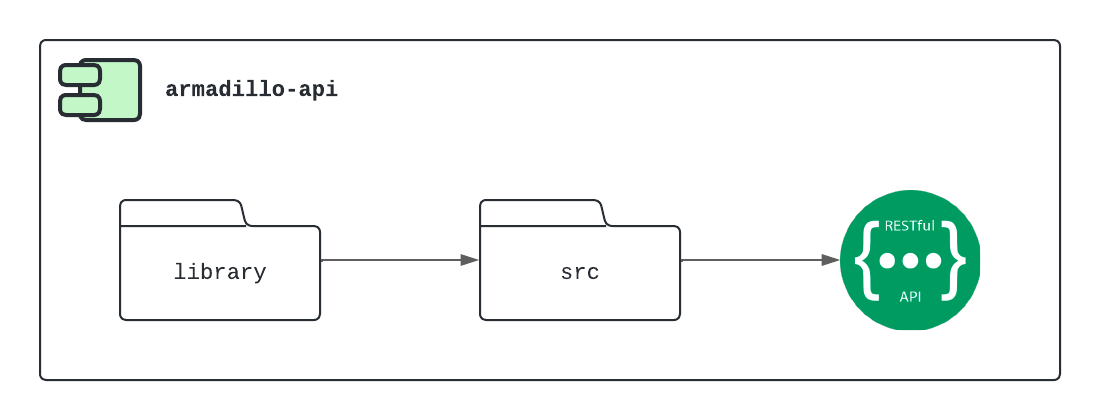
\includegraphics[width=\textwidth]{cap3_comp_armadillo.png}
		\caption{Estructura de los paquetes para el componente armadillo-api.}
		\label{fig:cap3_comp_armadillo}
	\end{figure}
	
\end{itemize}

\subsection{Fase 5: Integración de los componentes}

En la figura \ref{fig:cap3_integracion_componentes} se puede visualizar la comunicación entre todos los componentes que controlan el correcto funcionamiento de la extensión. El funcionamiento de los componentes es del a siguiente manera:

\begin{enumerate}
	\item \textbf{db-repository-tddt4iots:} Contiene todos los objetos necesarios para acceder a los datos de forma óptima.
	\item \textbf{ms-core-tddt4iots:} Mantiene separados los recursos reutilizables por toda la extensión, además de contener los DTO necesarios para las peticiones entre el cliente y el servidor.
	\item \textbf{ms-core-tddt4iots-openai:} Es el componente principal del proyecto, consumiendo los recursos de los componentes mencionados anteriormente, utilizados como dependencias mediante Maven.
	\item \textbf{ms\_core\_tddt4iots\_py:} Establece la comunicación con OpenAI y configura lo necesario para realizar entrenamientos e implementar los modelos.
	\item \textbf{armadillo-api:} API RestFul que interpreta casos de uso redactados en lenguaje de símbolos para obtener texto en lenguaje natural y crear archivos de entrenamiento.
\end{enumerate}

	\begin{figure}[H]  
		\centering
		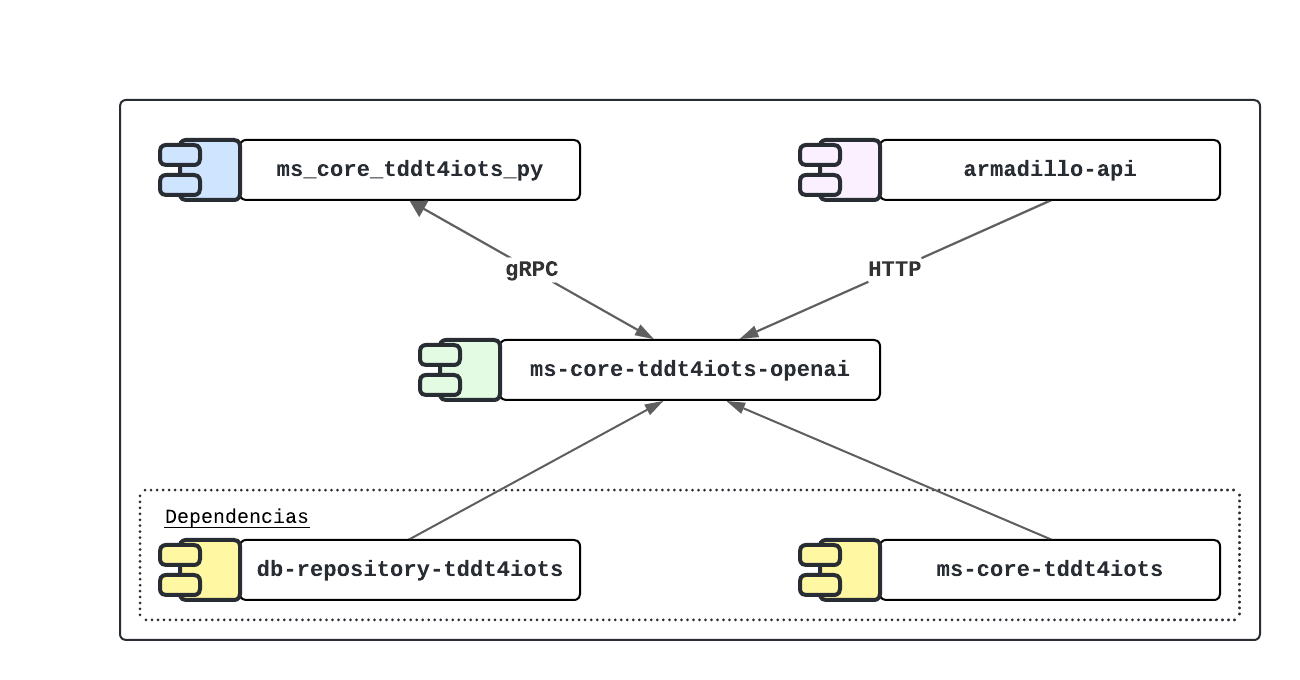
\includegraphics[width=\textwidth]{cap3_integracion_componentes.png}
		\caption{Componentes de la extensión.}
		\label{fig:cap3_integracion_componentes}
	\end{figure}


\section{Metodología para desarrollar la aplicación web}

La metodología Modelo-Vista-Controlador (MVC) es una de las arquitecturas de software más utilizadas en el desarrollo de aplicaciones web debido a su capacidad para separar las preocupaciones, facilitando así el mantenimiento y escalabilidad del proyecto. Esta metodología divide la aplicación en tres componentes principales: el Modelo, la Vista y el Controlador.

\begin{itemize}
	\item \textbf{Modelo: } Este componente representa la lógica de la aplicación y la estructura de datos. Es responsable de gestionar los datos de la aplicación, respondiendo a las solicitudes del controlador y actualizando la vista cuando la información cambia. El modelo interactúa con la base de datos y maneja las reglas de negocio.
	\item \textbf{Vista: } La vista es la capa de presentación de la aplicación. Su principal función es mostrar los datos del modelo al usuario en un formato adecuado y capturar la entrada del usuario. La vista es independiente de la lógica del negocio, lo que permite cambiar la interfaz de usuario sin afectar al resto de la aplicación.
	\item \textbf{Controlador: } El controlador actúa como intermediario entre el modelo y la vista. Recibe las entradas del usuario a través de la vista, las procesa (interactuando con el modelo si es necesario) y devuelve la salida adecuada a la vista. El controlador contiene la lógica de la aplicación que responde a las acciones del usuario y gestiona las rutas de la aplicación.
\end{itemize}

La implementación de la metodología MVC permite desarrollar aplicaciones web de manera más estructurada y organizada, facilitando la colaboración entre los desarrolladores y la implementación de nuevas funcionalidades de manera eficiente.

\subsection{Interfaces de la aplicación web}

La extensión de la herramienta case conllevo a realizar varios ajustes y desarrollar nuevas pantallas y funcionalidades que se adapten y cumplan con el objetivo de la investigación. En la figura \ref{fig:cap3_interfaz_001} se observa como el nombre de usuario dentro de la pantalla principal de la aplicación, se agrega una sombra de color verde. Esta sombra de color verde indica la nueva implementación que existe con los modelos de inteligencia artificial.

\begin{figure}[H]  
	\centering
	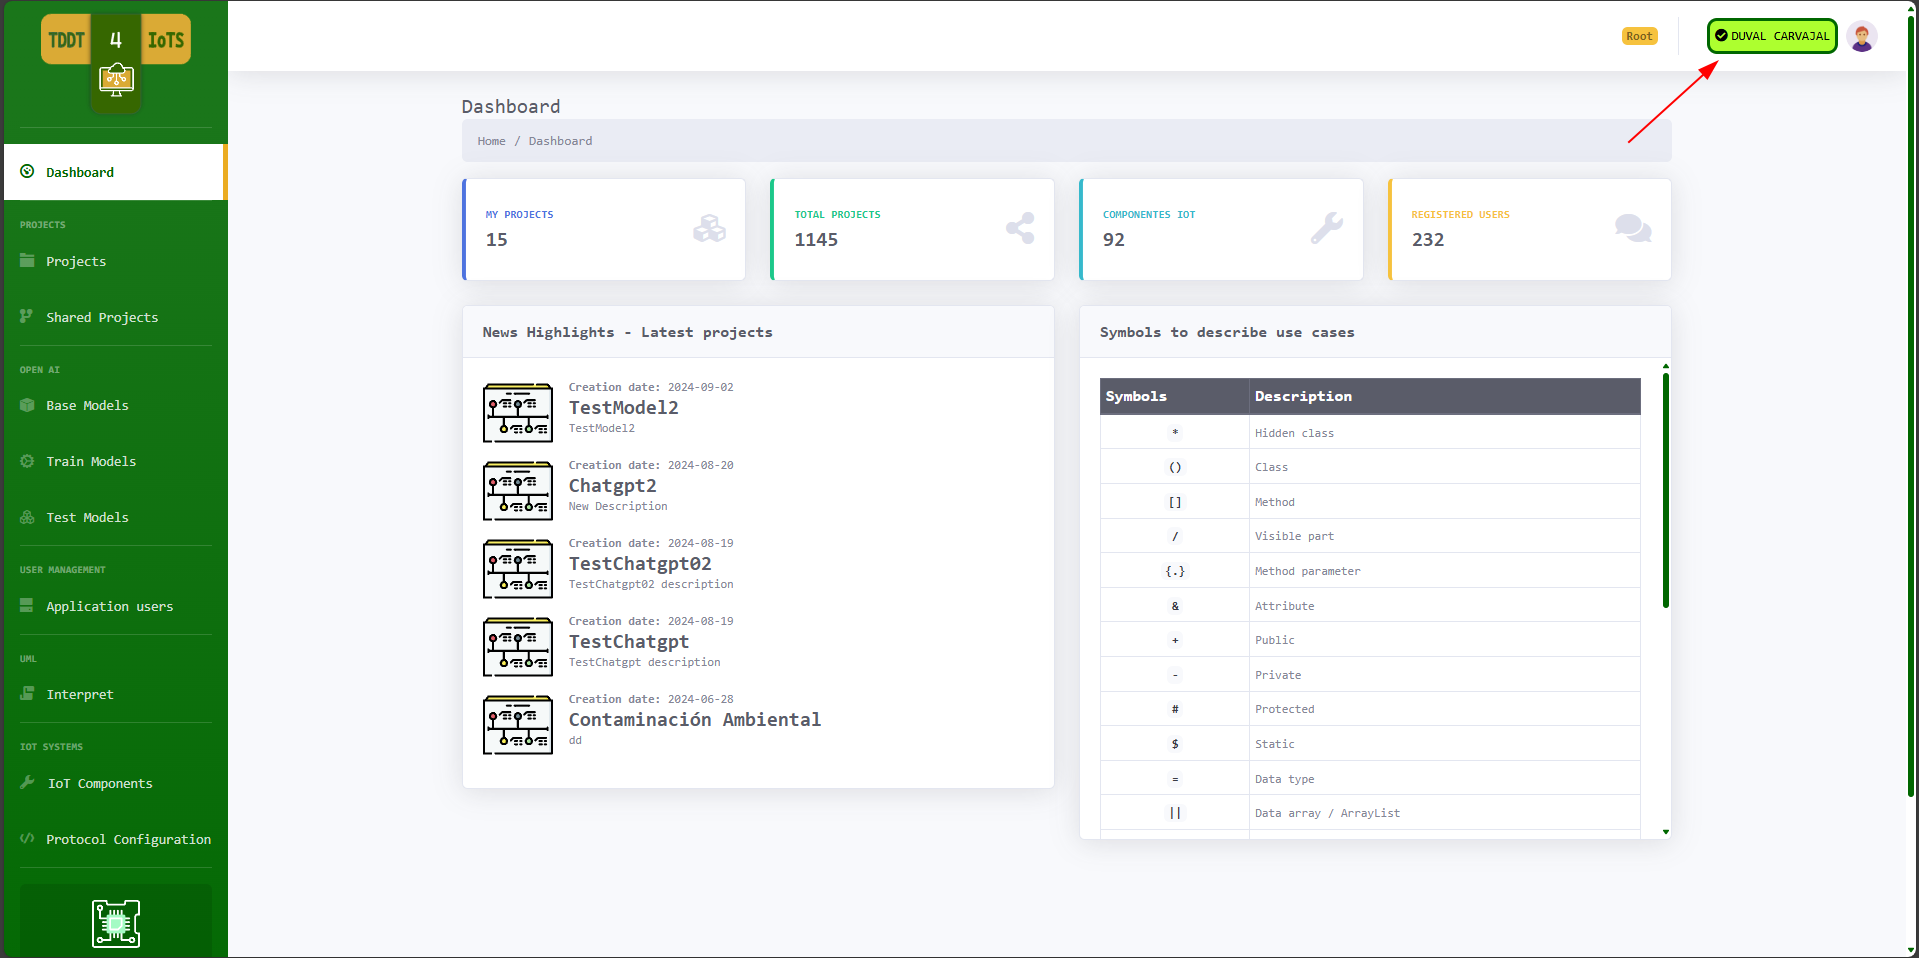
\includegraphics[width=\textwidth]{interfaz001.png}
	\caption{Interfaz principal de la aplicación.}
	\label{fig:cap3_interfaz_001}
\end{figure}

La figura \ref{fig:cap3_interfaz_002} muestra las nuevas opciones que se despliegan al dar click en el nombre de usuario. La opcion \textit{"Secret Key Open Ai"} permite poder ingresar la clave secreta de la api de OpenAi.

\begin{figure}[H]  
	\centering
	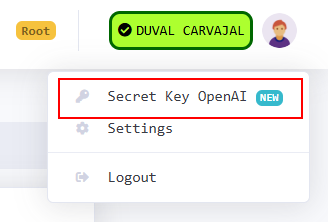
\includegraphics[width=250px]{interfaz002.png} 
	\caption{Nuevas opciones.}
	\label{fig:cap3_interfaz_002}
\end{figure}

En la figura \ref{fig:cap3_interfaz_003} se observa el formulario que aparecerá cuando ingresemos a la opción de \textit{"Secret Key Open Ai"}.

\begin{figure}[H]  
	\centering
	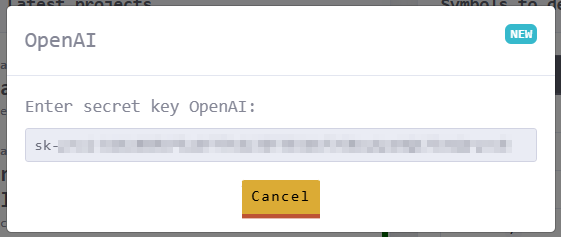
\includegraphics[width=300px]{interfaz003.png} 
	\caption{Formulario para ingresar la clave secreta de OpenAi.}
	\label{fig:cap3_interfaz_003}
\end{figure}

La figura \ref{fig:cap3_interfaz_004} muestra en en el recuadro rojo la opción para configurar los modelos de OpenAI disponibles dentro de la herramienta.
 
\begin{figure}[H]  
	\centering
	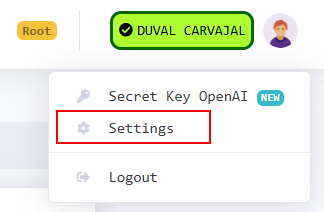
\includegraphics[width=250px]{interfaz004.png} 
	\caption{Nuevas opciones.}
	\label{fig:cap3_interfaz_004}
\end{figure}

Al acceder a la opción de \textit{"Settings"}, la opcion de \textit{"OpenAi"} muestra los modelos disponibles en la herramienta. El formulario está dividido en dos secciones (ver figura \ref{fig:cap3_interfaz_005}). En la primera sección, se visualizan los modelos base de la herramienta, destacándose en color azul el modelo base que ha sido seleccionado por el usuario. En la segunda sección, se muestra el tipo de uso que el usuario está aplicando al modelo. En este caso, el modelo base seleccionado está siendo utilizado específicamente para interpretar el texto natural enviado a través de las descripciones de los casos de uso.

\begin{figure}[H]  
	\centering
	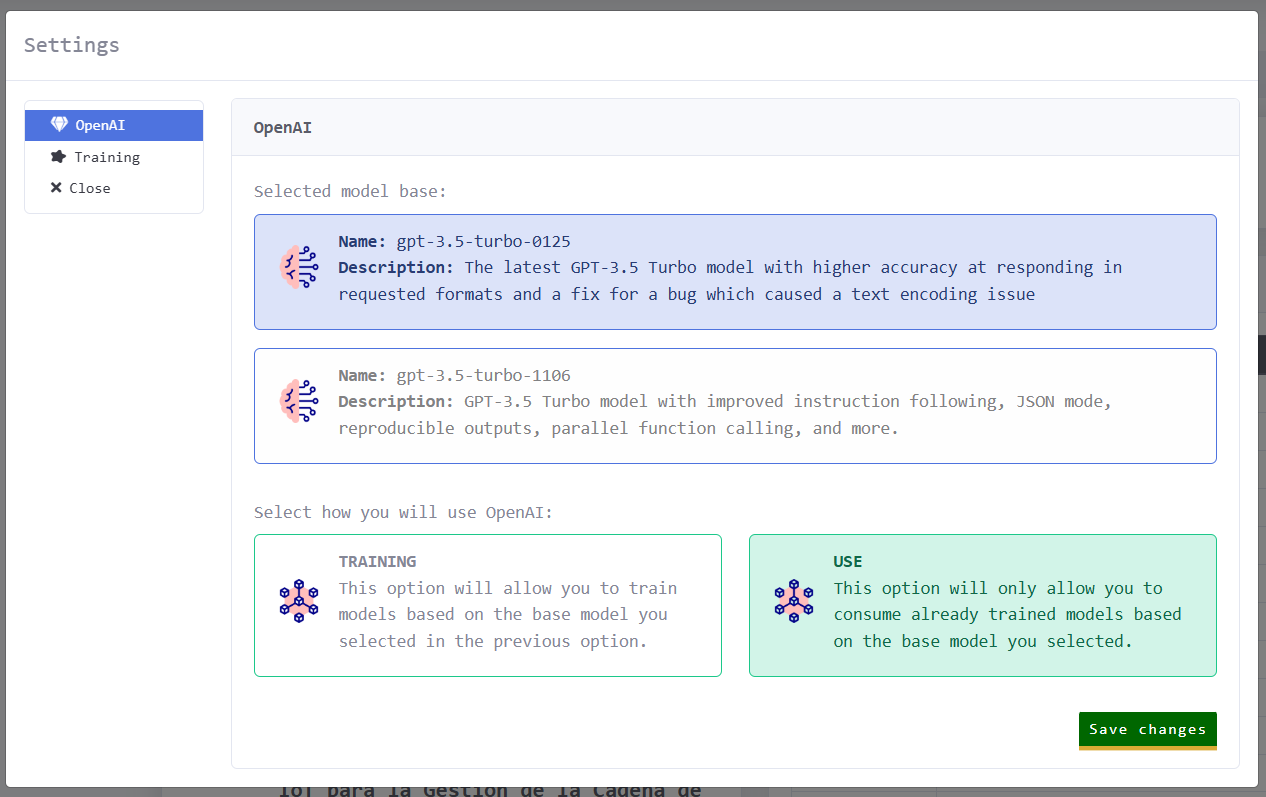
\includegraphics[width=\textwidth]{interfaz005.png} 
	\caption{Formulario de configuración de los modelos de OpenAi. Modelos base y el uso que le dará el usuario.}
	\label{fig:cap3_interfaz_005}
\end{figure}

La opción de \textit{"Training"} muestra la información sobre los entrenamientos realizados sobre le modelo base que se encuentra seleccionado. Además, se observa el nombre del usuario quien realizo el entrenamiento respectivo al modelo (ver figura \ref{fig:cap3_interfaz_006} y \ref{fig:cap3_interfaz_007}).

\begin{figure}[H]  
 	\centering
 	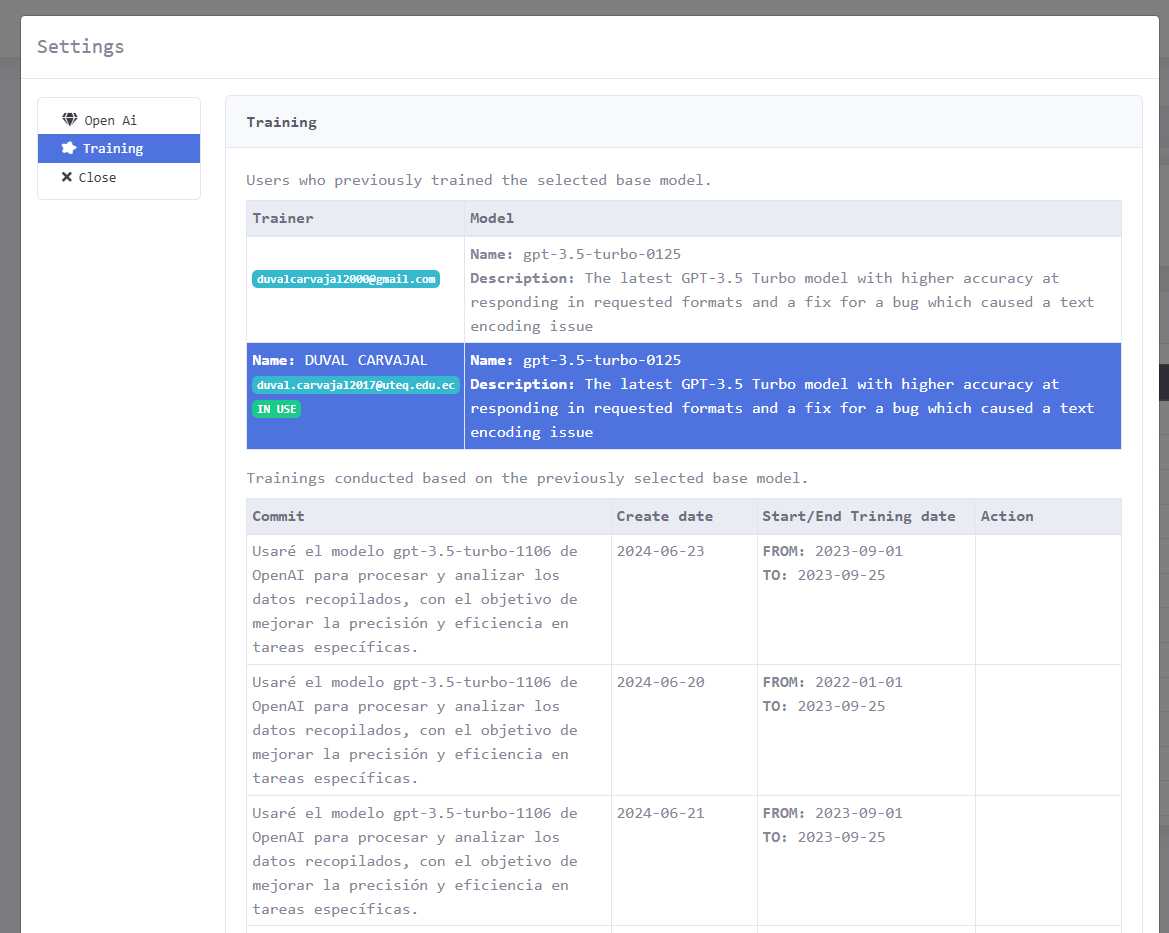
\includegraphics[width=270px]{interfaz006.png} 
 	\caption{Formulario de configuración de los modelos de OpenAi. Entrenamiento de los modelos base y su modelo seleccionado.}
 	\label{fig:cap3_interfaz_006}
\end{figure}

\begin{figure}[H]  
	\centering
	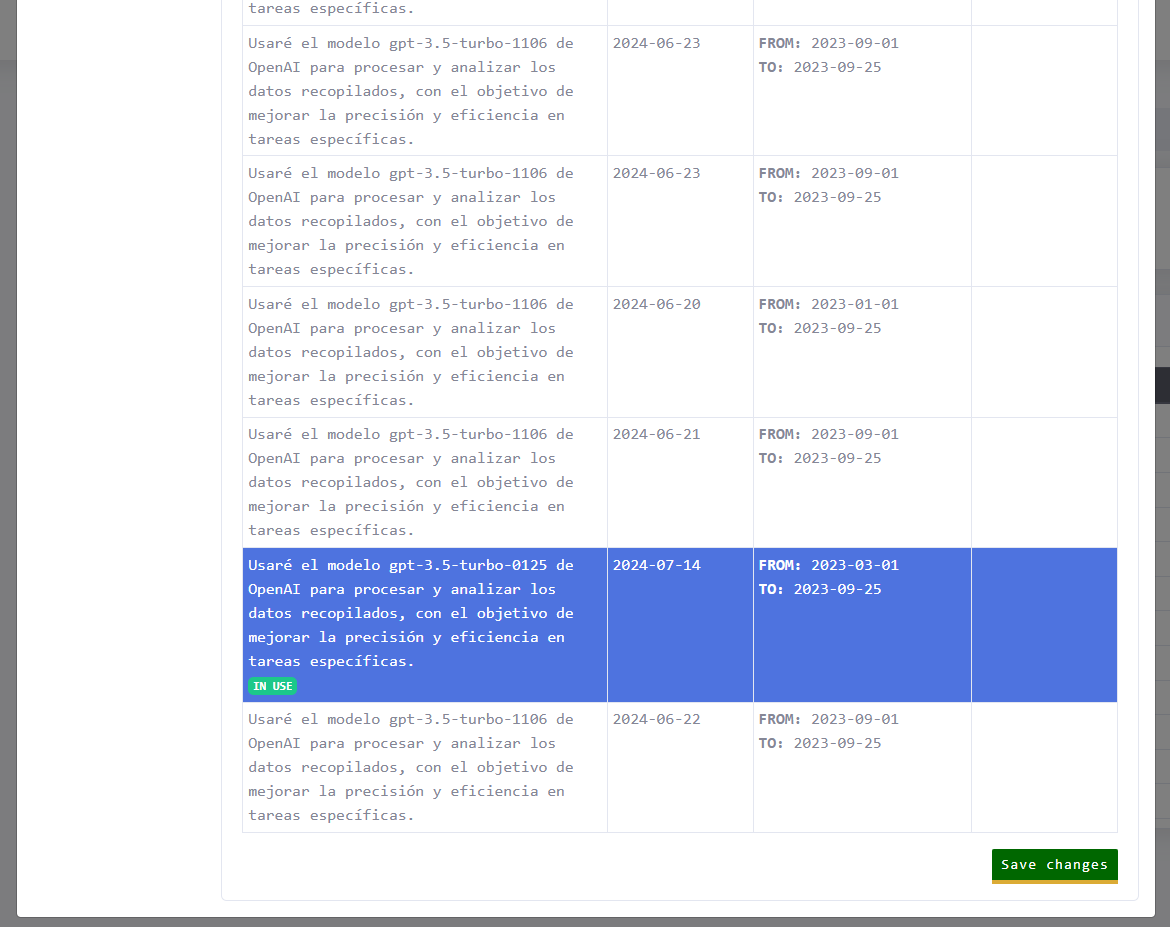
\includegraphics[width=270px]{interfaz007.png} 
	\caption{Formulario de configuración de los modelos de OpenAi. Entrenamiento de los modelos base y su modelo seleccionado.}
	\label{fig:cap3_interfaz_007}
\end{figure}

Dentro de la herramienta se agregaron 3 opciones al menú principal con el objetivo de gestionar los modelos base que podrán ser ingresados, los entrenamientos y otra opción para poder probar el modelo entrenado de forma independiente a los proyectos que tenga la herramienta. La figura \ref{fig:cap3_interfaz_008} muestra la opción \textit{"Base Models"} que permitirá ingresar los modelos base de OpenAi que se crean necesarios para ser utilizados por la herramienta.

\begin{figure}[H]  
	\centering
	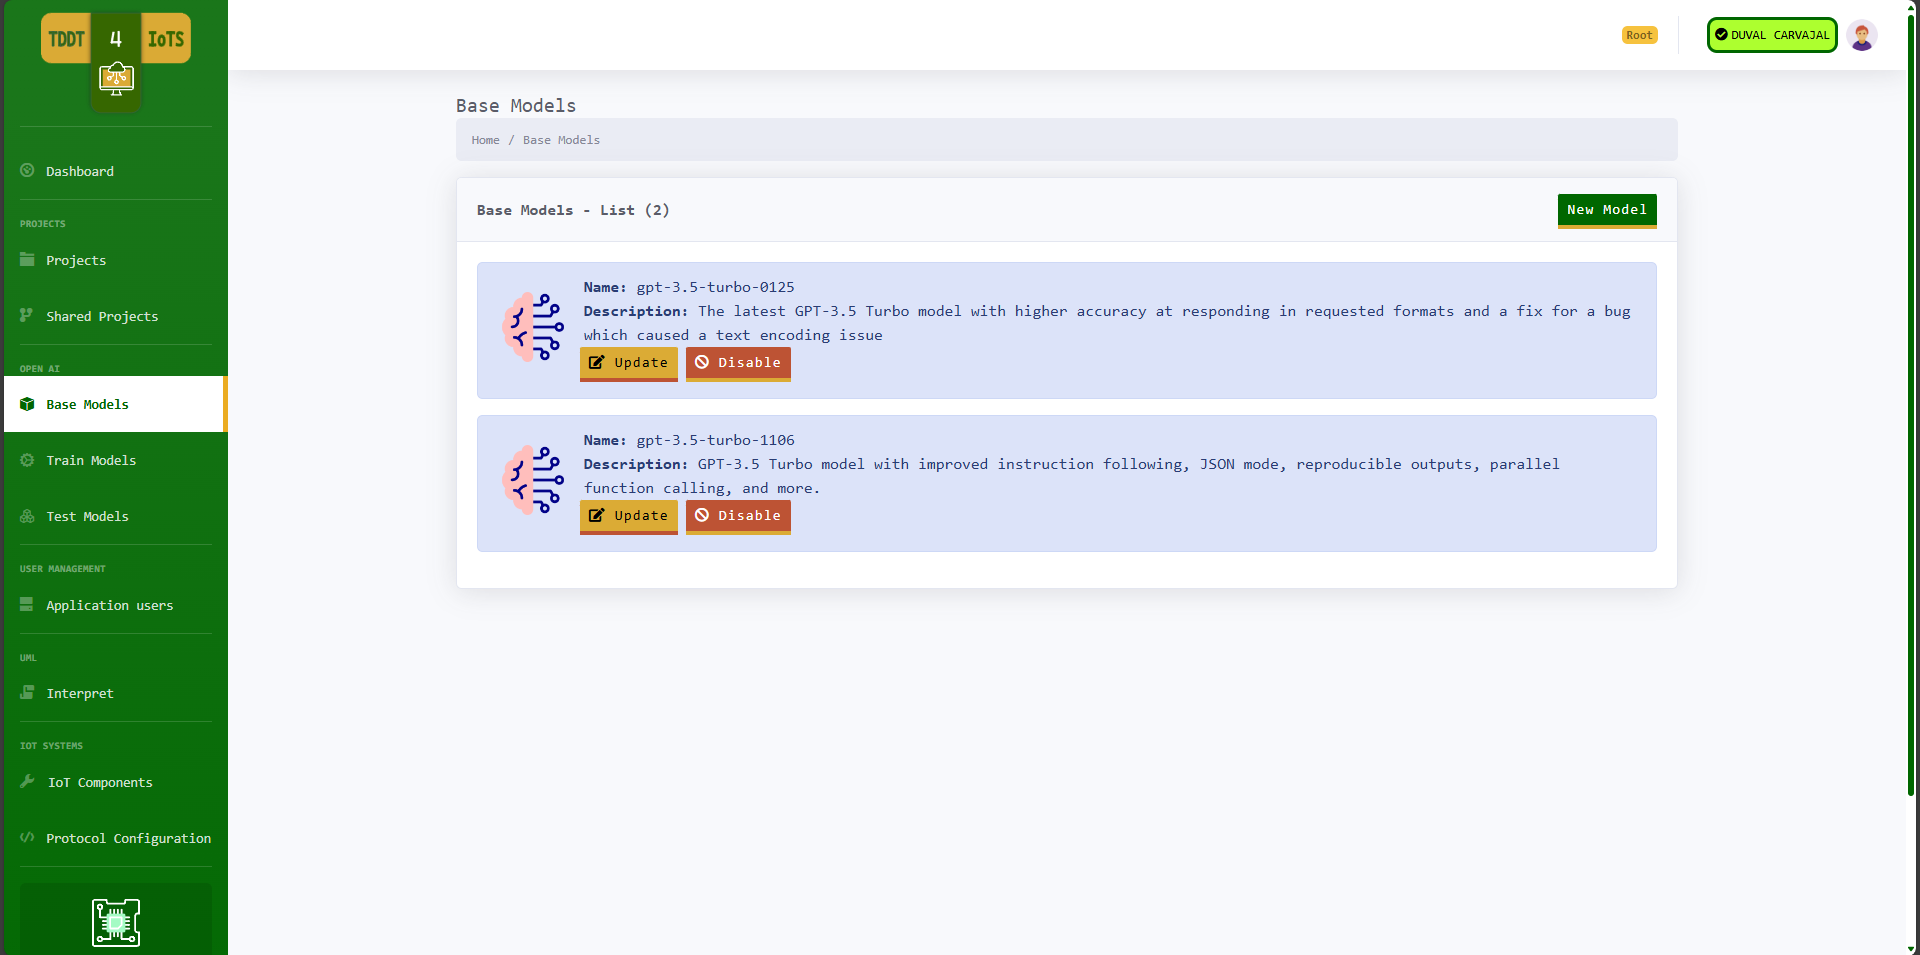
\includegraphics[width=300px]{interfaz008.png} 
	\caption{Opción para gestionar los modelos base de OpenAI dentro de la herramienta.}
	\label{fig:cap3_interfaz_008}
\end{figure}

La figura \ref{fig:cap3_interfaz_009} muestra la opción \textit{"Train models"}. En esta opción se podrán gestionar los entrenamientos al modelo base seleccionado. Se puede observar una lista de los entrenamientos y el estado en el que se encuentra o quedo cada entrenamiento que fue realizado desde la herramienta. Los datos para el entrenamiento son en base a los datos que actualmente se encontraron en la herramienta.  

\begin{figure}[H]  
	\centering
	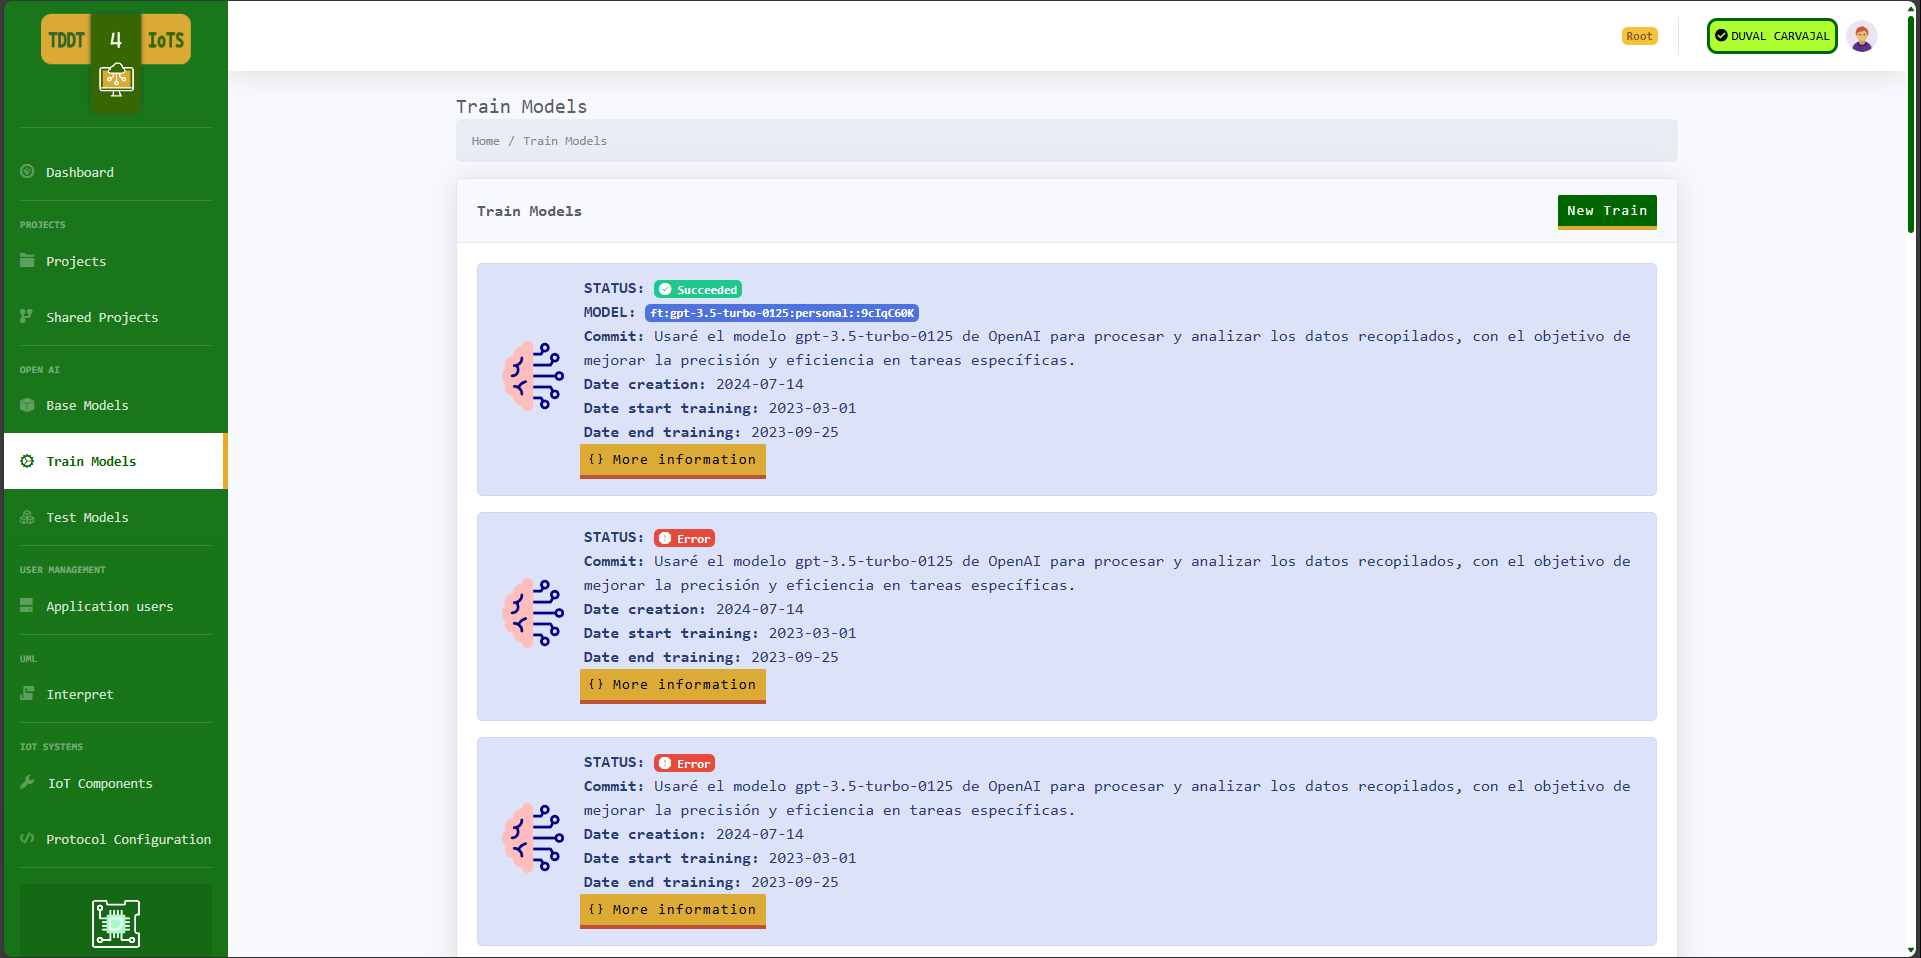
\includegraphics[width=300px]{interfaz009.png} 
	\caption{Opción para gestionar los entrenamientos de los modelos base de OpenAI dentro de la herramienta.}
	\label{fig:cap3_interfaz_009}
\end{figure} 

Para conocer mas información detallada sobre cada entrenamiento realizado, se puede ingresar a la opción de \textit{"More information"} (ver figura \ref{fig:cap3_interfaz_010}). Al ingresar a esa opción en la figura \ref{fig:cap3_interfaz_011} se observa  como se desplegara un formulario con el \textit{JSON} de respuesta devuelto por OpenAI del entrenamiento realizado. 

\begin{figure}[H]  
	\centering
	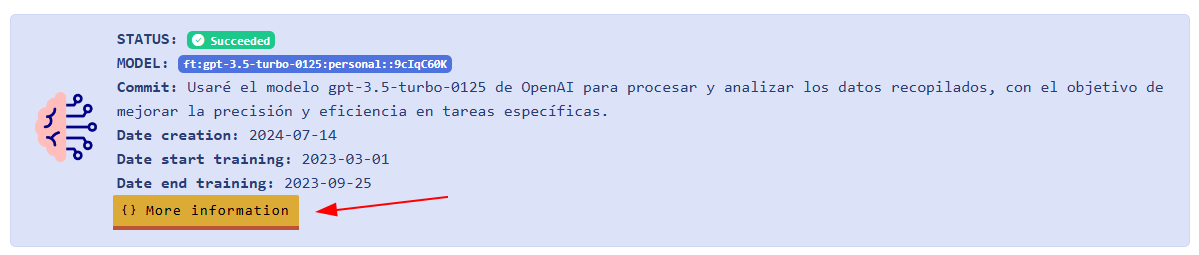
\includegraphics[width=300px]{interfaz010.png} 
	\caption{Entrenamiento realizado dentro de la herramienta y sus opciones disponibles.}
	\label{fig:cap3_interfaz_010}
\end{figure} 

\begin{figure}[H]  
	\centering
	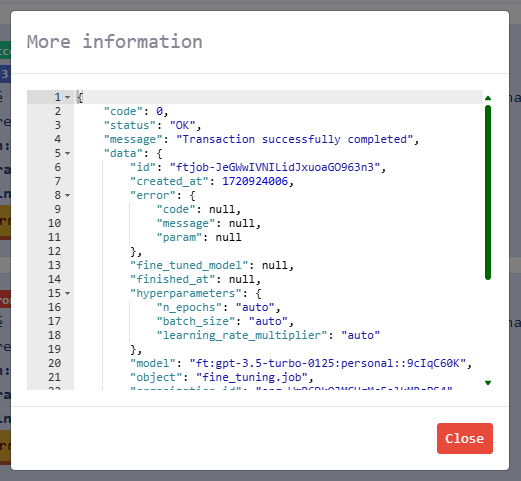
\includegraphics[width=250px]{interfaz011.png} 
	\caption{Información detallada del entrenamiento.}
	\label{fig:cap3_interfaz_011}
\end{figure}

La figura \ref{fig:cap3_interfaz_012} muestra la última opción denominada \textit{"Test Models"}. Esta opción permite al usuario probar el modelo seleccionado para utilizarlo dentro de la herramienta \textit{case}. Para realizar la prueba, solo se requiere proporcionar un texto en lenguaje natural que describa una parte de los casos de uso del sistema informático de interés. Luego, se espera la respuesta de OpenAI, y la herramienta genera el diagrama de clases correspondiente según la solicitud descrita en el texto enviado.
 
 \begin{figure}[H]  
 	\centering
 	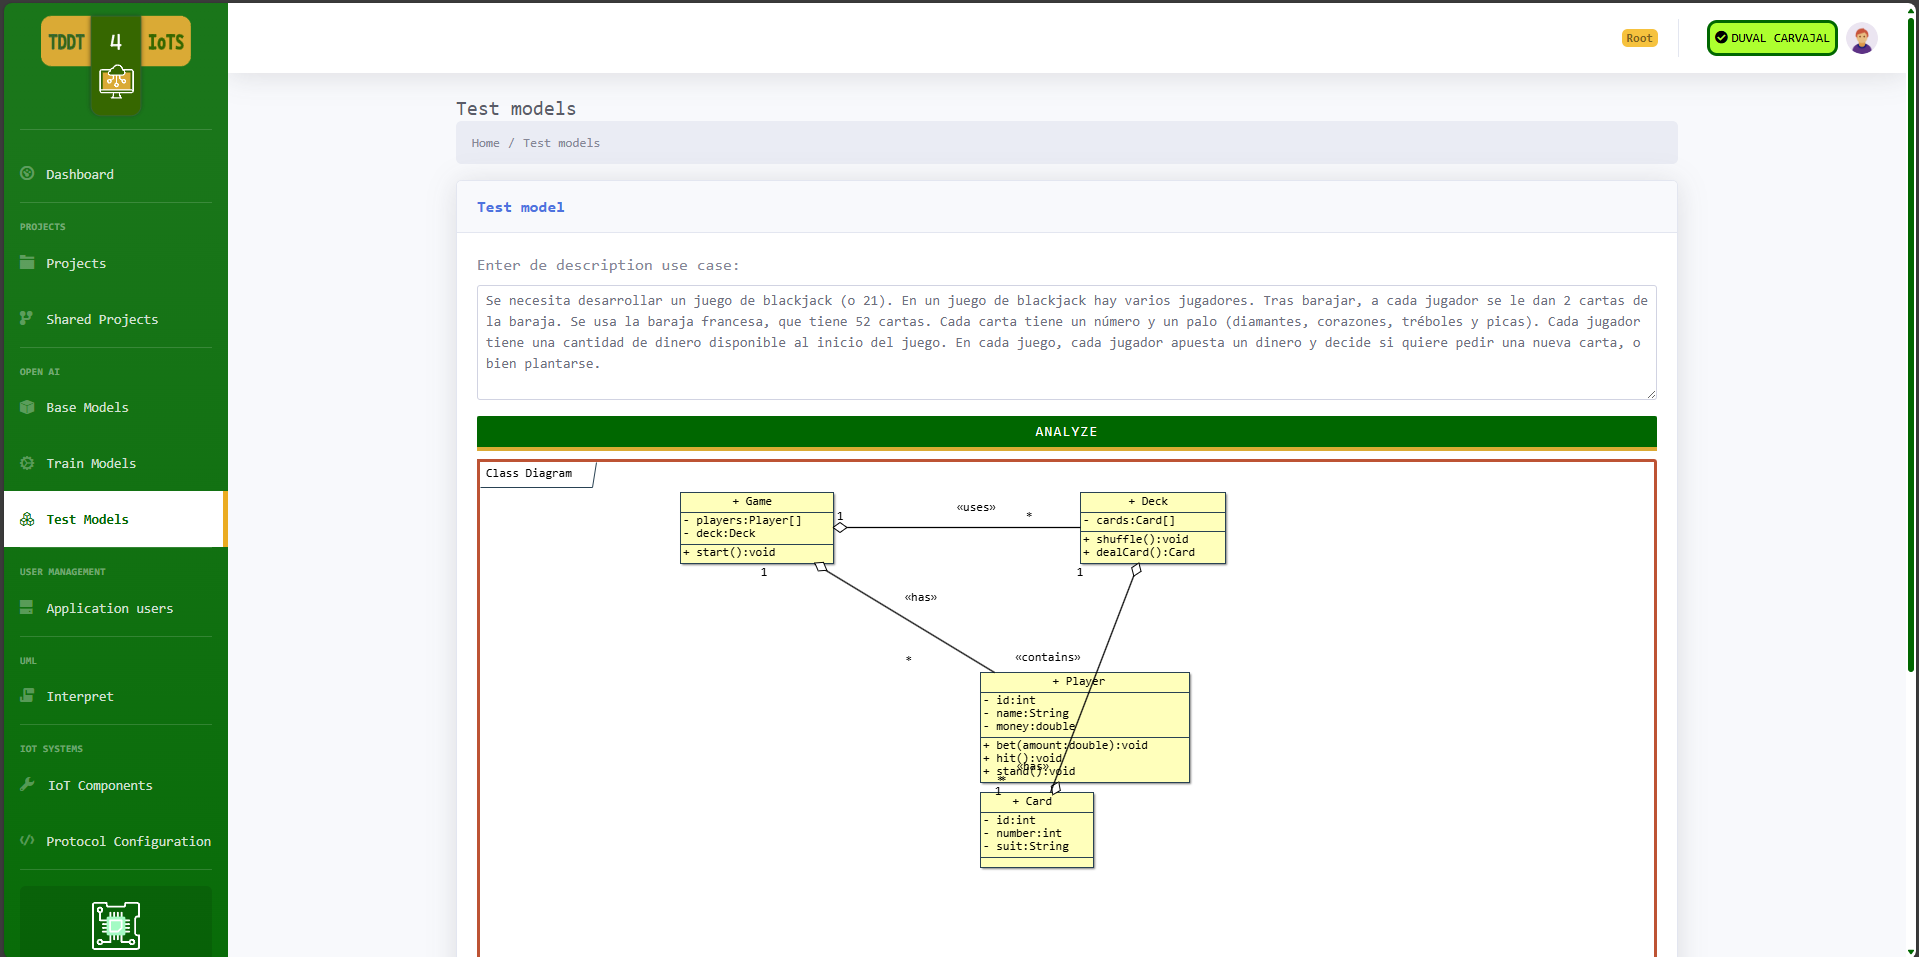
\includegraphics[width=\textwidth]{interfaz012.png} 
 	\caption{Prueba del modelo de OpenAI entrenado.}
 	\label{fig:cap3_interfaz_012}
 \end{figure}

Una vez que el modelo entrenado esté listo y se haya comprobado que puede analizar correctamente la descripción del caso de uso enviado, se puede proceder a la siguiente etapa de la herramienta. En esta fase, se utilizará el modelo con todas las descripciones de los casos de uso del sistema de interés para generar un diagrama de clases lo más ajustado al objetivo del sistema. En la figura \ref{fig:cap3_interfaz_013}, se muestra cómo la flecha señala una opción denominada \textit{"Activate OpenAI"}. Permite activar o desactivar el uso del modelo para analizar las descripciones de los casos de uso. Dado que la herramienta incluye un intérprete de descripciones de casos de uso, esta opción determina si se desea emplear el modelo en el análisis o no.


 \begin{figure}[H]  
	\centering
	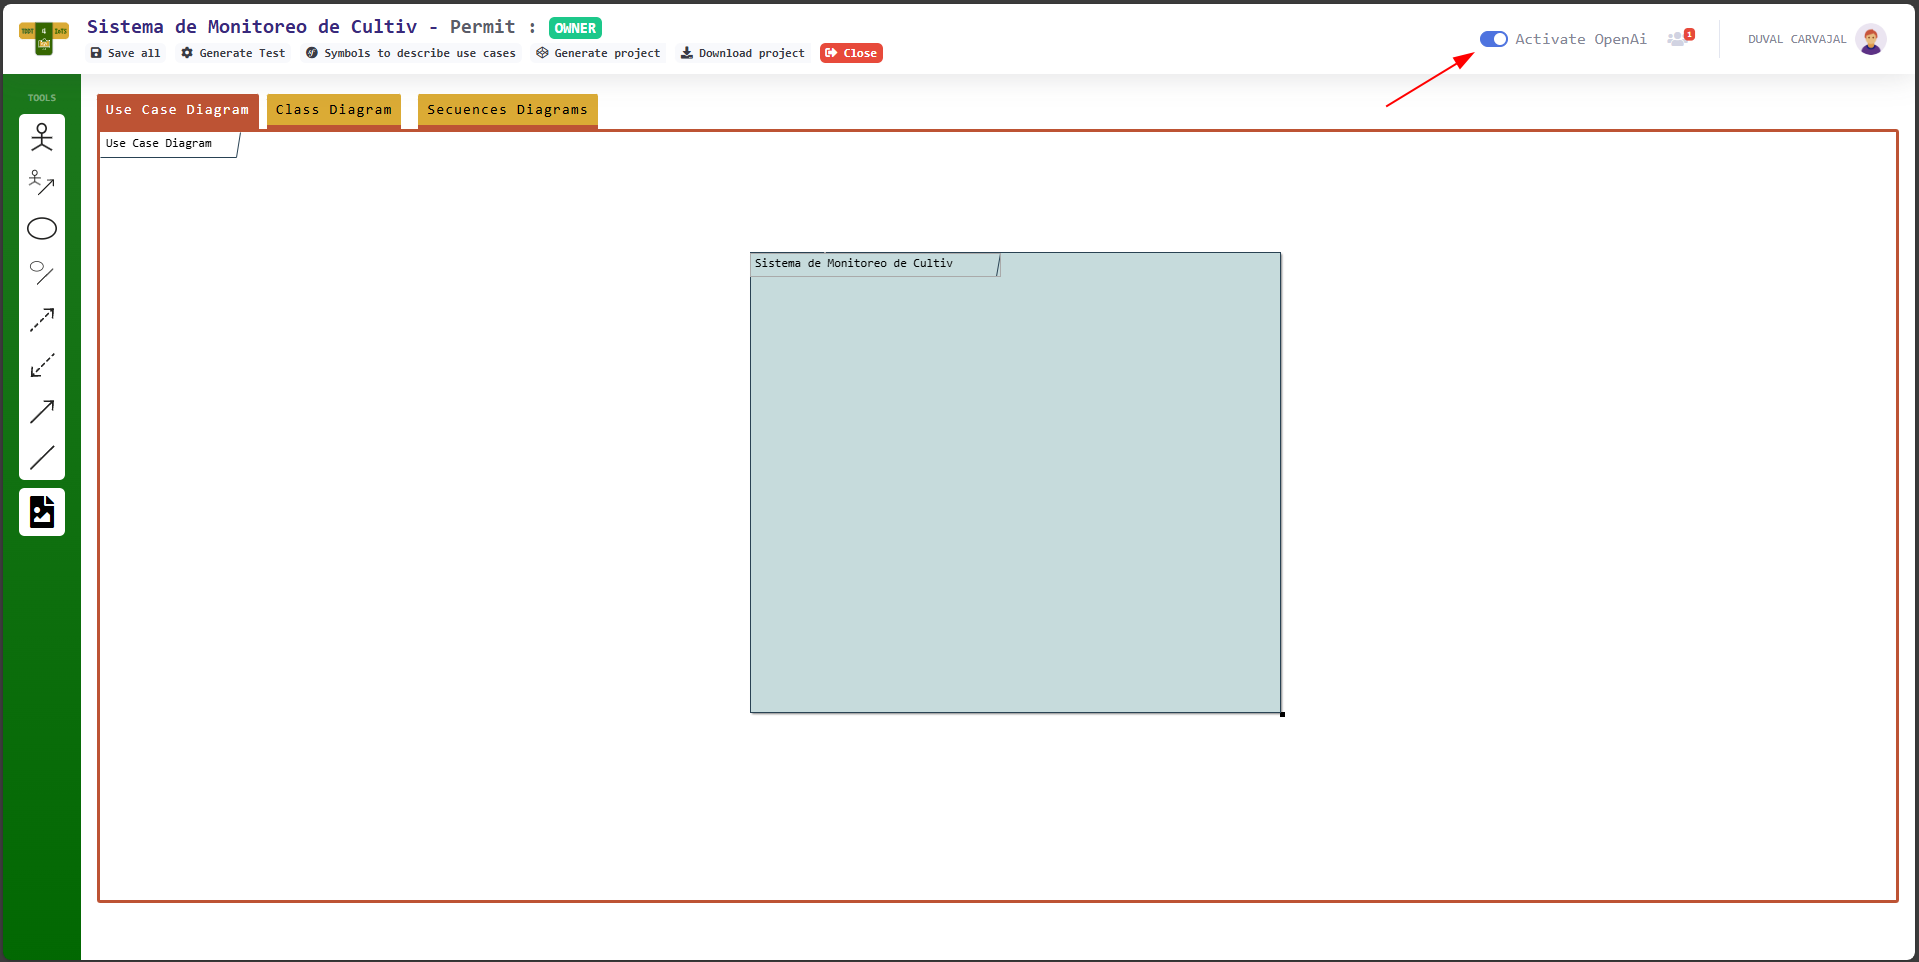
\includegraphics[width=\textwidth]{interfaz013.png} 
	\caption{Área para crear el diagrama de casos de uso e indicar si se usara el modelo de OpenAI.}
	\label{fig:cap3_interfaz_013}
\end{figure}

La figura \ref{fig:cap3_interfaz_014} muestra como la descripción del caso de uso actual esta ingresada con texto natural. Esperando que el modelo sea capaz de interpretar cada sección del caso de uso y también todos los casos de uso que permitan crear el diagrama de clases. 

 \begin{figure}[H]  
	\centering
	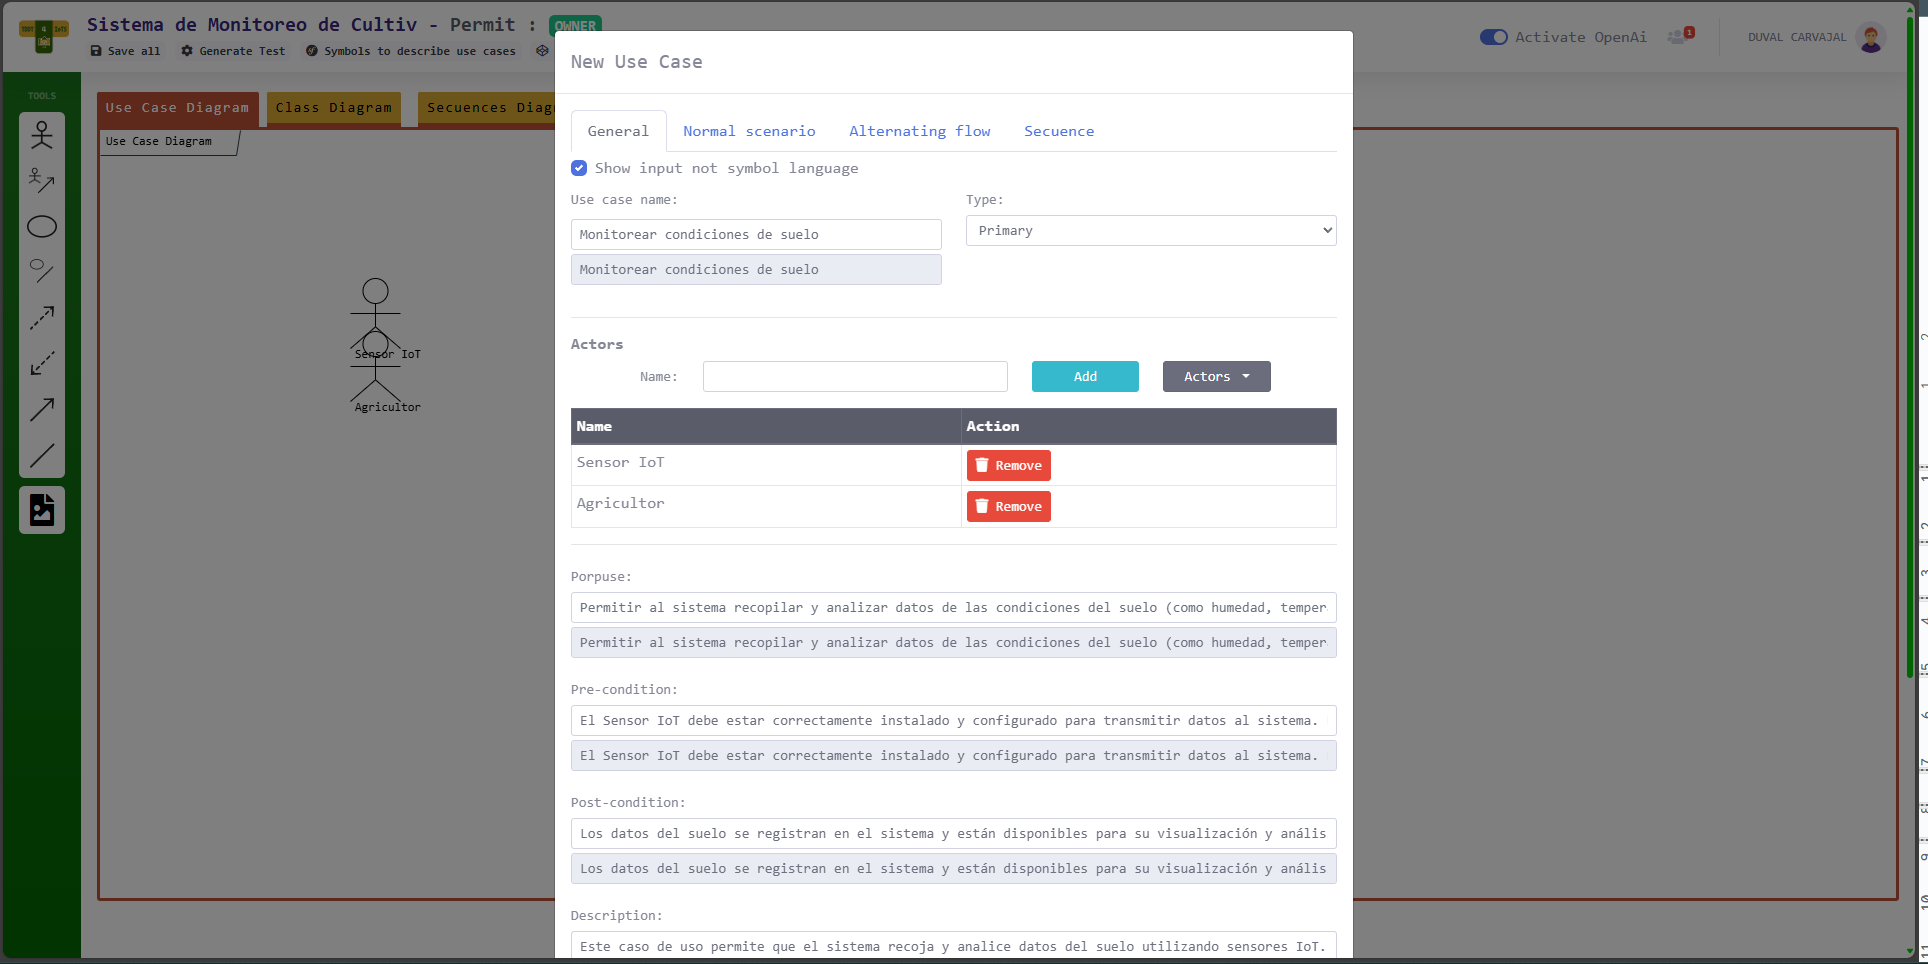
\includegraphics[width=\textwidth]{interfaz014.png} 
	\caption{Formulario para ingresar la descripción de cada caso de uso del sistema.}
	\label{fig:cap3_interfaz_014}
\end{figure}

Cuando el modelo este trabajando sobre los casos de uso se podrá observar una leyenda que indicara el momento que OpenAI esta analizando las descripciones de los casos de uso (ver figura \ref{fig:cap3_interfaz_015}). 

 \begin{figure}[H]  
	\centering
	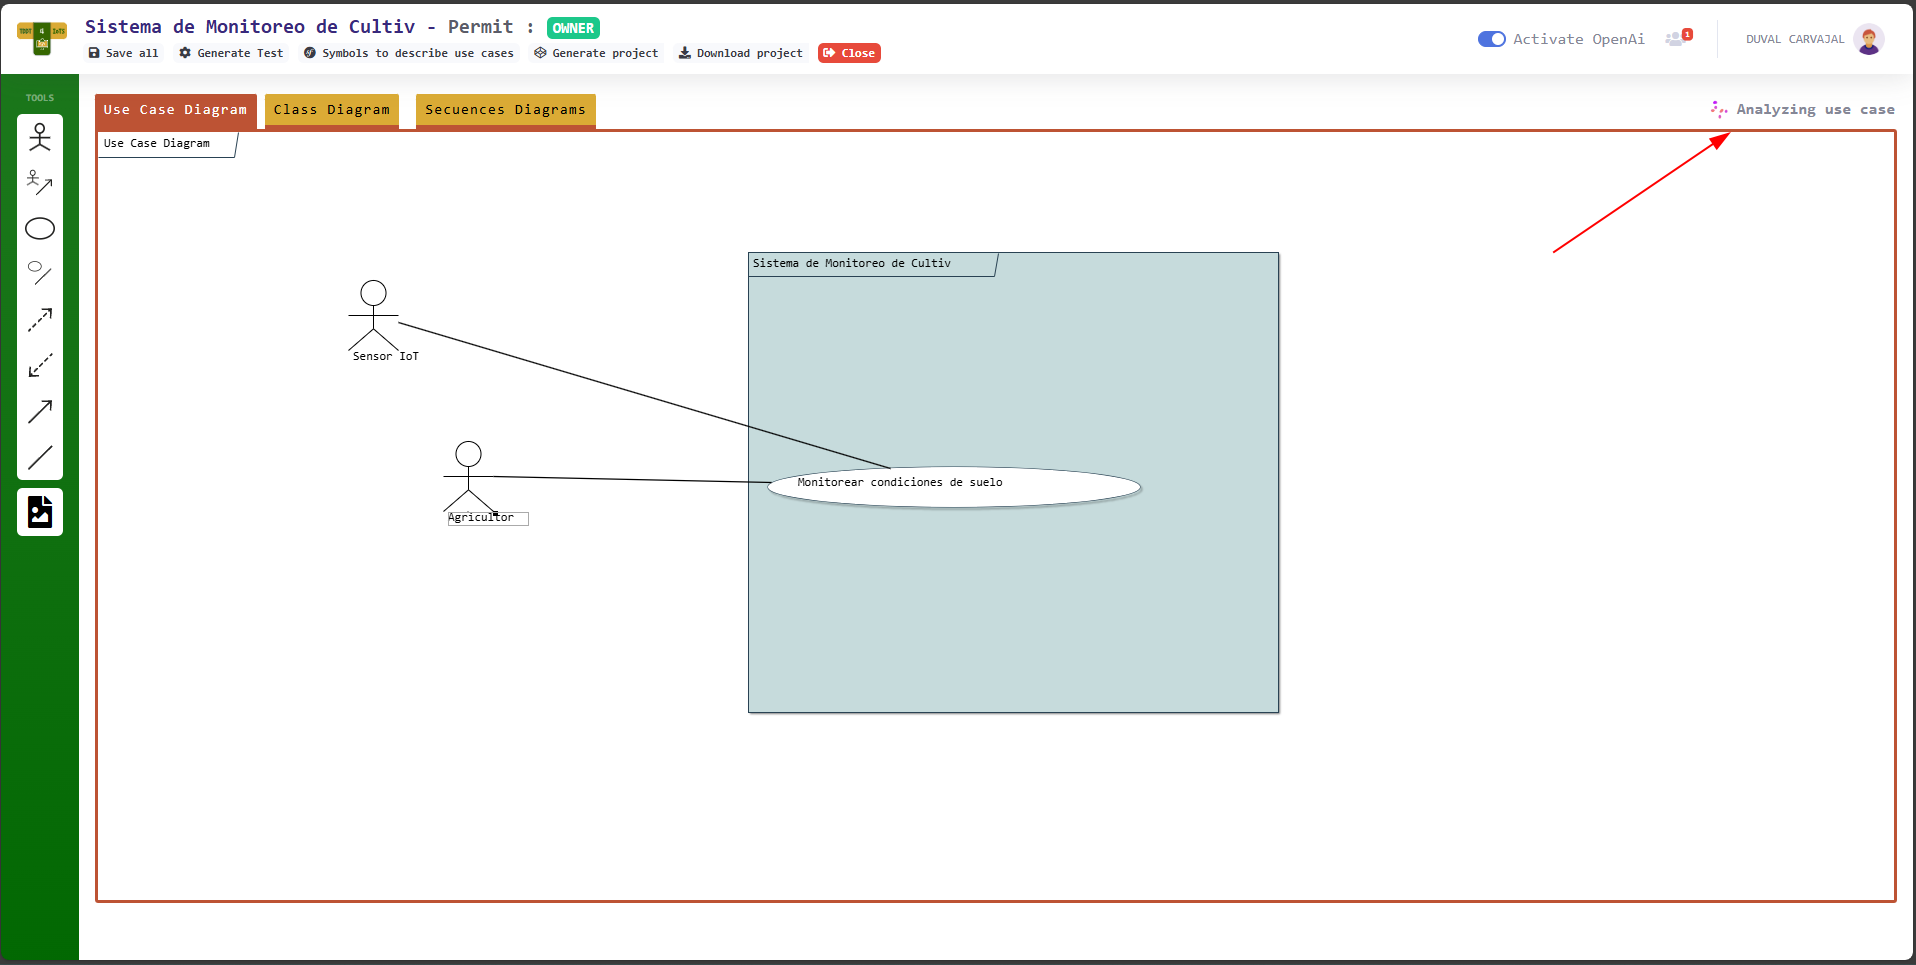
\includegraphics[width=\textwidth]{interfaz015.png} 
	\caption{Estado del modelo al analizar los casos de uso.}
	\label{fig:cap3_interfaz_015}
\end{figure}

Finalmente en la figura \ref{fig:cap3_interfaz_016} se muestra como la herramienta fue capaz de generar el diagrama de clases mediante las descripciones de los casos de uso del sistema a desarrollar.

 \begin{figure}[H]  
	\centering
	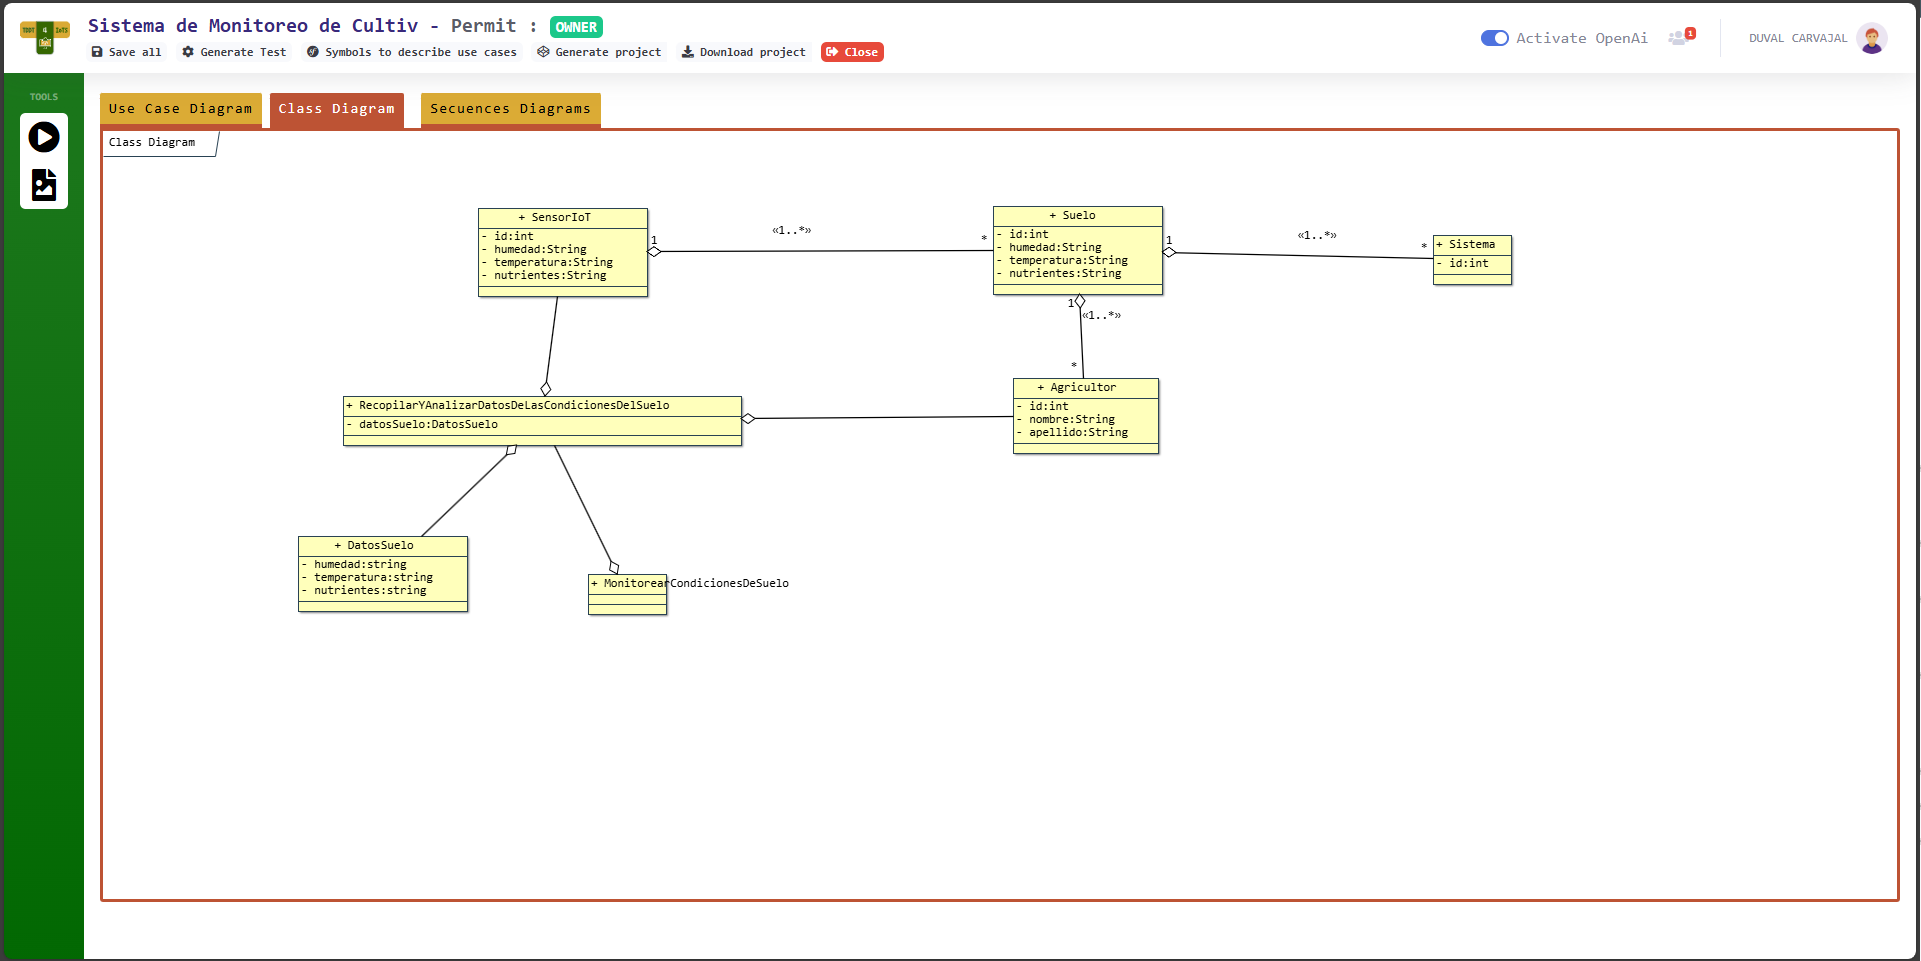
\includegraphics[width=\textwidth]{interfaz016.png} 
	\caption{Diagrama de clases generado por la herramienta y el modelo de OpenAI.}
	\label{fig:cap3_interfaz_016}
\end{figure}

\subsection{Evaluación de la extensión dentro de la aplicación web}

Para evaluar la efectividad de la herramienta, se contactó a 15 estudiantes de la Universidad Técnica Estatal de Quevedo, Ecuador. A estos estudiantes se les solicitó que utilizaran la herramienta y cargaran uno de los proyectos en los que estuvieran trabajando durante sus estudios, creando el diagrama de casos de uso para su sistema IoT. Una vez redactadas las descripciones de los casos de uso en lenguaje natural, la herramienta analizará cada proyecto y generará automáticamente el diagrama de clases correspondiente a cada estudiante.

A cada estudiante se le envió la invitación a 1 documento1 compartido1 para que puedan ingresar las descripciones de los casos de uso y tener documentado todos los proyectos que se ingresaron en la herramienta para su respectiva evaluación. En la figura \ref{fig:cap3_evaluacion_001} se muestra el documento de texto que fue compartido y se observan las descripciones de los casos de uso de cada proyecto.

 \begin{figure}[H]  
	\centering
	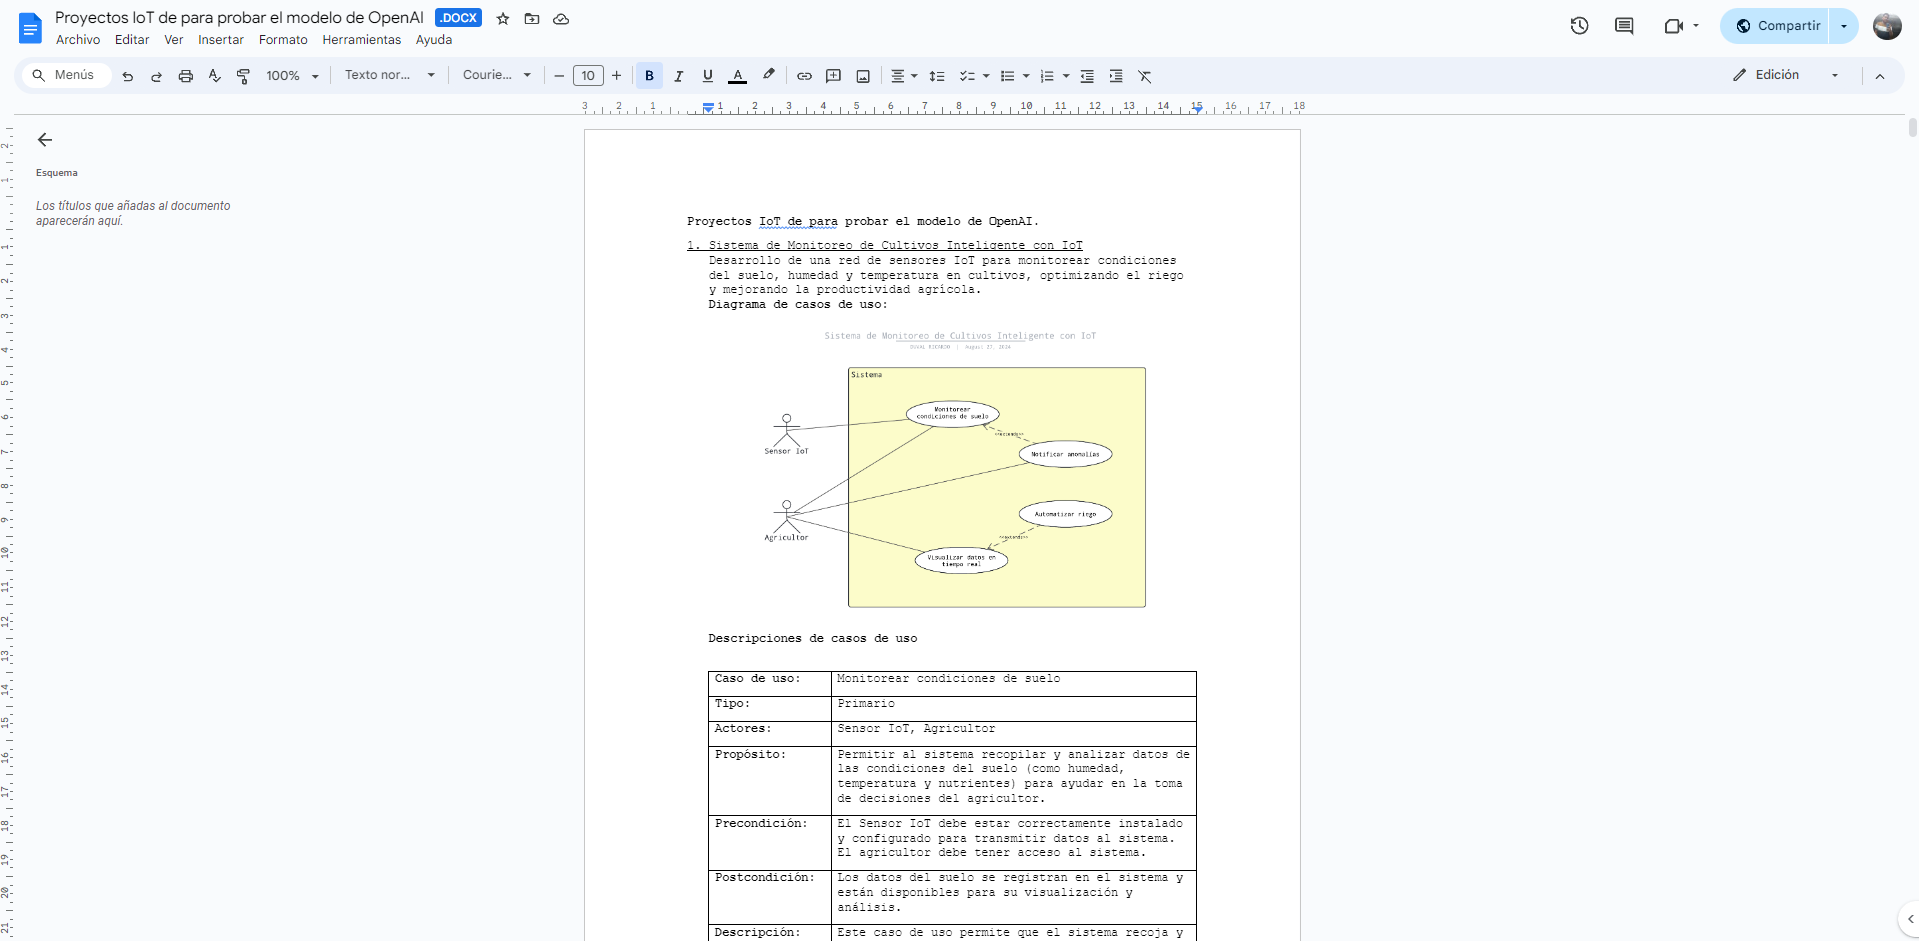
\includegraphics[width=\textwidth]{evaluacion001.png} 
	\caption{Documento de texto compartido con todos los proyectos ingresados para evaluar la extensión de la herramienta.}
	\label{fig:cap3_evaluacion_001}
\end{figure}

Para las descripciones de los casos de uso se les indico una plantilla para que puedan documentarla y sea mas fácil ingresarlos dentro de la herramienta. A continuación se mostrara un ejemplo de uno de los proyectos a evaluar.

\textbf{Proyecto: } Sistema de Monitoreo de Cultivos Inteligente con IoT \\
\textbf{Descripción: } Desarrollo de una red de sensores IoT para monitorear condiciones del suelo, humedad y temperatura en cultivos, optimizando el riego y mejorando la productividad agrícola. 

\begin{longtable}{|p{5cm}|p{5cm}|}
	\hline
	\multicolumn{2}{|c|}{\textbf{Caso de uso: Monitorizar condiciones de suelo}} \\
	\hline
	\textbf{Tipo:} & Primario \\
	\hline
	\textbf{Actores:} & Sensor IoT, Agricultor \\
	\hline
	\textbf{Propósito:} & Permitir al sistema recopilar y analizar datos de las condiciones del suelo (como humedad, temperatura y nutrientes) para ayudar en la toma de decisiones del agricultor. \\
	\hline
	\textbf{Precondición:} & El Sensor IoT debe estar correctamente instalado y configurado para transmitir datos al sistema. El agricultor debe tener acceso al sistema. \\
	\hline
	\textbf{Postcondición:} & Los datos del suelo se registran en el sistema y están disponibles para su visualización y análisis. \\
	\hline
	\textbf{Descripción:} & Este caso de uso permite que el sistema recoja y analice datos del suelo utilizando sensores IoT. Los datos recopilados son accesibles para el agricultor en tiempo real, y se pueden usar para la toma de decisiones sobre el manejo de los cultivos. \\
	\hline
	\multicolumn{2}{|c|}{\textbf{Flujo normal}} \\
	\hline
	\textbf{Actor} & \textbf{Sistema} \\
	\hline
	1. El Sensor IoT recopila datos del suelo en intervalos regulares. & \\
	\hline
	& 2. El sistema recibe y almacena los datos. \\
	\hline
	& 3. El sistema analiza los datos para detectar patrones o tendencias. \\
	\hline
	4. El agricultor puede acceder a los datos en tiempo real a través del sistema. & \\
	\hline
	\multicolumn{2}{|c|}{\textbf{Flujo alternativo}} \\
	\hline
	\textbf{Actor} & \textbf{Sistema} \\
	\hline
	1. Si el Sensor IoT no puede transmitir los datos, el sistema genera una notificación al agricultor para tomar acciones correctivas. & \\
	\hline
\end{longtable}

\begin{longtable}{|p{5cm}|p{5cm}|}
	\hline
	\multicolumn{2}{|c|}{\textbf{Caso de uso: Notificar anomalías}} \\
	\hline
	\textbf{Tipo:} & Primario \\
	\hline
	\textbf{Actores:} & Agricultor \\
	\hline
	\textbf{Propósito:} & Informar al agricultor sobre cualquier condición anómala detectada en el suelo para que pueda tomar medidas inmediatas. \\
	\hline
	\textbf{Precondición:} & El sistema debe estar monitoreando las condiciones del suelo activamente y contar con una base de datos de condiciones normales. \\
	\hline
	\textbf{Postcondición:} & El agricultor es informado de la anomalía y puede tomar acciones correctivas. \\
	\hline
	\textbf{Descripción:} & El sistema detecta automáticamente cualquier condición anómala en el suelo y notifica al agricultor para que pueda actuar rápidamente. Este proceso asegura que el agricultor esté siempre informado de posibles problemas que puedan afectar sus cultivos. \\
	\hline
	\multicolumn{2}{|c|}{\textbf{Flujo normal}} \\
	\hline
	\textbf{Actor} & \textbf{Sistema} \\
	\hline
	& 1. El sistema detecta una condición anómala en los datos del suelo (ej. baja humedad, presencia de plagas). \\
	\hline
	& 2. El sistema genera una notificación automática. \\
	\hline
	3. El agricultor recibe la notificación en su dispositivo. & \\
	\hline
	\multicolumn{2}{|c|}{\textbf{Flujo alternativo}} \\
	\hline
	\textbf{Actor} & \textbf{Sistema} \\
	\hline
	1. Si el agricultor no responde a la notificación, el sistema envía recordatorios o escala la notificación a otros medios (como SMS). & \\
	\hline
\end{longtable}

\begin{longtable}{|p{5cm}|p{5cm}|}
	\hline
	\multicolumn{2}{|c|}{\textbf{Caso de uso: Visualizar datos en tiempo real}} \\
	\hline
	\textbf{Tipo:} & Primario \\
	\hline
	\textbf{Actores:} & Agricultor \\
	\hline
	\textbf{Propósito:} & Permitir al agricultor acceder a una interfaz que muestre los datos actuales de las condiciones del suelo, facilitando el monitoreo continuo. \\
	\hline
	\textbf{Precondición:} & El sistema debe estar recibiendo y procesando datos del Sensor IoT en tiempo real. \\
	\hline
	\textbf{Postcondición:} & Los datos se muestran correctamente y están actualizados en la interfaz del usuario. \\
	\hline
	\textbf{Descripción:} & El agricultor puede monitorear las condiciones del suelo en tiempo real mediante una interfaz visual proporcionada por el sistema, lo que le permite tomar decisiones informadas sobre el manejo de sus cultivos. \\
	\hline
	\multicolumn{2}{|c|}{\textbf{Flujo normal}} \\
	\hline
	\textbf{Actor} & \textbf{Sistema} \\
	\hline
	1. El agricultor accede al sistema a través de su dispositivo. & \\
	\hline
	& 2. El sistema muestra los datos en una interfaz gráfica en tiempo real. \\
	\hline
	3. El agricultor puede observar y analizar los datos para tomar decisiones inmediatas. & \\
	\hline
	\multicolumn{2}{|c|}{\textbf{Flujo alternativo}} \\
	\hline
	\textbf{Actor} & \textbf{Sistema} \\
	\hline
	1. Si la conexión con el Sensor IoT falla, el sistema muestra una advertencia y proporciona los últimos datos disponibles. & \\
	\hline
\end{longtable}

\begin{longtable}{|p{5cm}|p{5cm}|}
	\hline
	\multicolumn{2}{|c|}{\textbf{Caso de uso: Automatizar riego}} \\
	\hline
	\textbf{Tipo:} & Primario \\
	\hline
	\textbf{Actores:} & Agricultor \\
	\hline
	\textbf{Propósito:} & Automatizar el proceso de riego basado en los datos del suelo, optimizando el uso de agua y asegurando que las plantas reciban la cantidad adecuada de humedad. \\
	\hline
	\textbf{Precondición:} & El sistema debe tener acceso a un controlador de riego automatizado y los datos del Sensor IoT deben estar disponibles. \\
	\hline
	\textbf{Postcondición:} & El riego se activa o desactiva automáticamente según las condiciones del suelo. \\
	\hline
	\textbf{Descripción:} & Este caso de uso permite al sistema tomar decisiones automatizadas sobre el riego de cultivos basándose en los datos del suelo, optimizando así los recursos hídricos y garantizando la salud de las plantas. \\
	\hline
	\multicolumn{2}{|c|}{\textbf{Flujo normal}} \\
	\hline
	\textbf{Actor} & \textbf{Sistema} \\
	\hline
	& 1. El sistema analiza los datos del Sensor IoT y determina si el suelo necesita riego. \\
	\hline
	& 2. Si se requiere riego, el sistema activa el sistema de riego automatizado. \\
	\hline
	& 3. El sistema monitorea el riego y lo detiene una vez que se alcanzan las condiciones óptimas. \\
	\hline
	\multicolumn{2}{|c|}{\textbf{Flujo alternativo}} \\
	\hline
	\textbf{Actor} & \textbf{Sistema} \\
	\hline
	1. Si el sistema de riego no responde, el sistema genera una notificación. & \\
	\hline
\end{longtable}

La figura \ref{fig:cap3_proyecto_001} muestra el diagrama de casos de uso del proyecto indicado.

 \begin{figure}[H]  
	\centering
	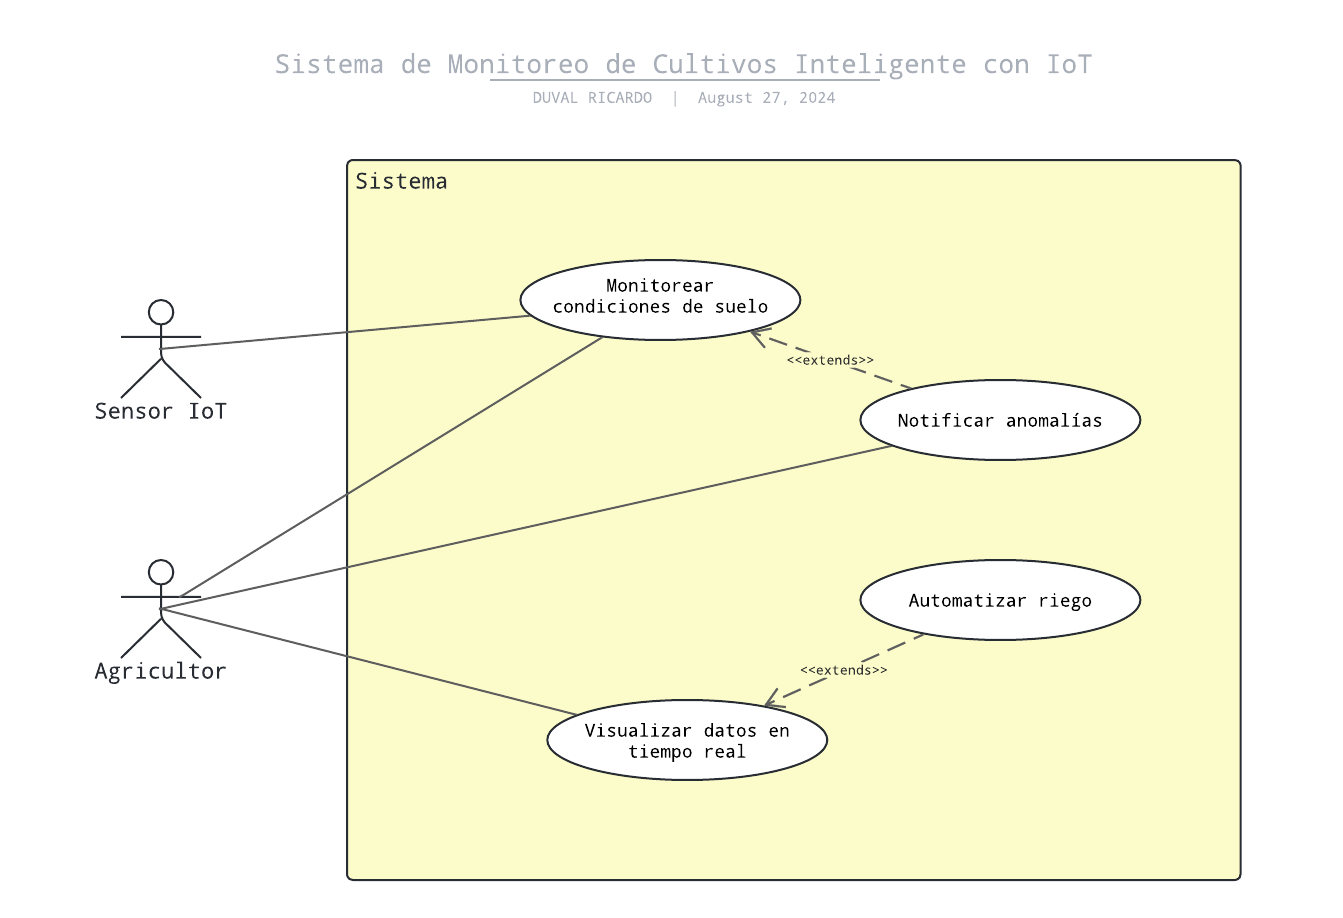
\includegraphics[width=\textwidth]{proyecto001.png} 
	\caption{Diagrama de casos de uso para el Sistema de Monitoreo de Cultivos Inteligente con IoT.}
	\label{fig:cap3_proyecto_001}
\end{figure}

Todos los proyectos que sirvieron para evaluar la extensión están realizados de esta forma, con el objetivo de obtener información lo mas apegado a la realidad. Dichos proyectos son trabajos de los estudiantes que presentaran en sus asignaturas respectivas.
\chapter{Resultados y discusión}\label{chapter:resultados}

Durante la implementación del proyecto, se evaluaron diversas tecnologías con el objetivo de seleccionar aquella que mejor se ajustara a los plazos de desarrollo y permitiera cumplir los objetivos establecidos. Aunque inicialmente se consideró la creación de un modelo de inteligencia artificial desde cero utilizando Python, los resultados indicaron que el tiempo necesario para entrenar el modelo y estabilizar sus respuestas era considerablemente elevado, lo que hacía inviable esta opción dentro de los plazos previstos.

Por otro lado, la implementación de modelos preentrenados, como los ofrecidos por OpenAI, resultó ser una alternativa mucho más eficiente. Estos modelos proporcionaron respuestas consistentes y claras tras un proceso de ajuste mínimo. Los resultados reflejan que, aunque fue necesario un grado de entrenamiento para adaptar los modelos a los objetivos específicos del proyecto, el tiempo total de desarrollo y ajuste fue significativamente menor en comparación con el desarrollo de un modelo desde cero. Además, la integración de estos modelos con la herramienta CASE fue fluida, lo que facilitó alcanzar los resultados esperados en un marco temporal reducido.

Para verificar el desempeño de los modelos de OpenAI integrados en la herramienta CASE, se realizó una prueba piloto con 15 estudiantes, quienes ingresaron descripciones de casos de uso relacionados con Sistemas IoT. Posteriormente, se realizó una encuesta para evaluar la satisfacción de los estudiantes y determinar si la nueva implementación de la herramienta CASE fue útil para su aprendizaje en el área de Software.

Los resultados de la encuesta, que se presentan a continuación mediante gráficos generados en R para facilitar su visualización, revelan la percepción de los estudiantes sobre la efectividad de la herramienta. Estos hallazgos permiten comprender de manera más lógica y clara los resultados obtenidos, destacando la mejora gracias a la extensión de la herramienta CASE mediante los modelos de OpenAI.

La figura \ref{fig:cap4_resultados} muestra los resultados obtenidos de la encuesta y a continuación analizaremos cada uno de ellos:

 \begin{figure}[H]  
	\centering
	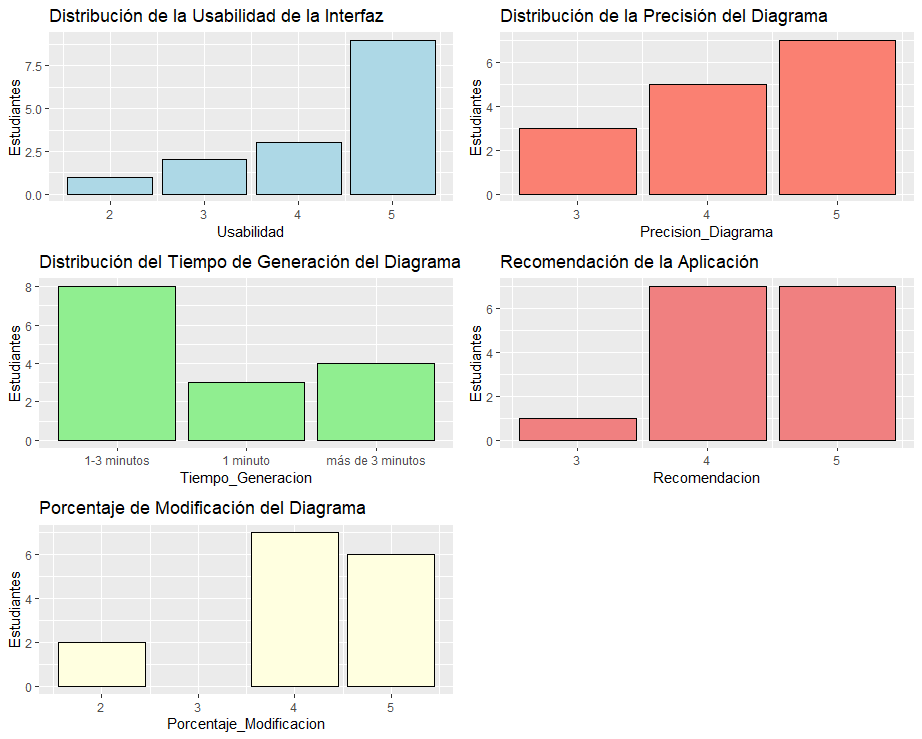
\includegraphics[width=\textwidth]{resultados.png} 
	\caption{Resultados de la encuesta.}
	\label{fig:cap4_resultados}
\end{figure}

\section{Distribución de la Usabilidad de la Interfaz}

Este gráfico muestra que la mayoría de los estudiantes (aproximadamente 8) calificaron la usabilidad de la interfaz con un 5, lo que indica una alta satisfacción con la interfaz de usuario. Un menor número de estudiantes calificó la usabilidad con 3 y 4, mientras que solo unos pocos le dieron una calificación más baja (2).

\textbf{Interpretación}: Esto sugiere que la interfaz de la herramienta es bien valorada por la mayoría de los usuarios, lo cual es un indicador positivo de la facilidad de uso del sistema implementado.

\section{Distribución de la Precisión del Diagrama}

La mayoría de los estudiantes calificaron la precisión del diagrama generado con un 5 (el puntaje más alto), seguido por un número significativo que le otorgó un 4. Solo algunos estudiantes dieron una calificación de 3 y ninguno puntuó por debajo de esto.

\textbf{Interpretación}: Los usuarios perciben que los diagramas generados por la herramienta tienen un alto nivel de precisión, lo que sugiere que el sistema cumplió bien con sus expectativas en cuanto a la representación de los casos de uso.

\section{Distribución del Tiempo de Generación del Diagrama}

La mayor parte de los estudiantes (aproximadamente 8) reportaron que el tiempo de generación del diagrama fue entre 1 y 3 minutos. Un menor número de estudiantes indicó que el tiempo fue de un minuto o de más de tres minutos.

\textbf{Interpretación}: La mayoría de los estudiantes percibió que el tiempo de generación del diagrama fue razonable y adecuado para el contexto del uso de la herramienta. Sin embargo, un pequeño grupo experimentó tiempos de generación más largos, lo que podría ser una oportunidad de mejora en la optimización de la herramienta.

\section{Recomendación de la Aplicación}

La gran mayoría de los estudiantes calificó la recomendación de la aplicación con un 4 o 5, lo que sugiere que recomendarían su uso a otros. Solo uno o dos estudiantes dieron una calificación de 3.

\textbf{Interpretación}: Esto indica una alta satisfacción general con la herramienta, lo cual es un resultado importante que refleja la utilidad percibida y la disposición de los usuarios a recomendarla.

\section{Porcentaje de Modificación del Diagrama}

Este gráfico muestra que la mayoría de los estudiantes realizaron modificaciones moderadas al diagrama, puntuando entre 4 y 5 en cuanto al porcentaje de modificación necesario. Algunos usuarios indicaron que se requirieron menos modificaciones (calificación de 3), y solo un estudiante reportó un porcentaje bajo de modificaciones.

\textbf{Interpretación}: Aunque los diagramas generados fueron precisos, aún se requirieron modificaciones para ajustarse completamente a los casos de uso. Esto indica que el sistema genera diagramas que están cercanos a la solución final, pero que necesitan pequeños ajustes por parte de los usuarios.

En general, los resultados indican que la herramienta implementada, que utiliza los modelos preentrenados de OpenAI integrados en la herramienta CASE, fue bien recibida por los estudiantes. La interfaz fue evaluada como fácil de usar, los diagramas generados tuvieron una buena aceptación, y los tiempos de generación fueron adecuados para la mayoría de los casos. Además, la mayoría de los usuarios indicaron que recomendarían la herramienta a otros. Aunque los diagramas generados necesitaban algunas modificaciones, estas eran mínimas, lo que refleja un buen desempeño en términos de exactitud.

\chapter{Conclusiones}\label{chapter:conclusiones}

Debes describir las conclusiones generales del trabajo, pero también debes cubrir qué objetivos se han cubierto. Para ello revisa la sección de \nameref{section:objetivos} (Sección \ref{section:objetivos}).
Por último cierra el trabajo, y si tienes planes de continuar, menciona los trabajos futuros.

% ------------------------------------------------------------


% Puedes descomentar esta línea para pruebas con la bibliografía,
% pero ¡¡¡en el trabajo final debes comentarla!!!
% \nocite{*}

\bibliography{bibliografia}\addcontentsline{toc}{chapter}{Bibliografía}
\bibliographystyle{ieeetr}

% Comenta esta sección si no tienes apéndices
\appendix
\chapter{Planificación y gestión del proyecto}

El Apéndice \thechapter\  puede incluirse como recomendación si se ha realizado un proyecto de tipo práctico práctico de desarrollo del software.

De forma general se puede incluir la especificación requerimientos del proyecto, la información sobre stakeholders del proyecto, la justificación (interés, oportunidad, coste/beneficio…), etc.

En cuanto a la planificación: se indicarán las diferentes tareas a desarrollar durante el proyecto ordenadas cronológicamente.

En cuanto a la descripción: breve definición de las tareas indicando su relación con los requisitos del proyecto, método de trabajo, tecnologías a utilizar para desarrollar cada tarea, posibles obstáculos y riesgos.

En cuanto a la validación: qué método se utilizará para validar el proyecto (si se trata de desarrollo de software, indicando métricas referidas a "code coverage", etc., pruebas unitarias, etc.).

En cuanto al estudio de costes y sostenibilidad: se indicarán las horas de programador necesarias para llevarlo a cabo, gasto en recursos, bibliografía, tiempos de conexión, etc. 

En cuanto a la temporización, lo suyo es un Diagrama de Gantt donde quede claro el tiempo invertido en la realización de cada una de las tareas y su secuenciación/entrelazamiento a los largo de los meses de relización del proyecto.

Finalmente se acabará justificando la sostenibilidad de los productos software generados en cuanto a costes de prueba y mantenimiento del software.

Una posible estructuración  de la gestión y planificación del proyecto podría ser en las siguientes subsecciones:

\section{Metodología/Ciclo de vida} 

\section{Herramientas y plataformas utilizadas para el desarrollo del proyecto}

\section{Costes del proyecto}

\section{Gestión del proyecto. Planificación temporal. Diagrama de Gantt}



\chapter{Innovación}

El Apéndice \thechapter\  puede ser recomendable incluir en los casos en los que se realice un proyecto práctico de desarrollo del software en los que se quiera hacer referencia a la posible innovación en el marco empresarial.

En caso positivo, se recomienda una posible estructuración en las siguientes subsecciones:

\section{Estudio del Mercado}
Contenido del estudio del mercado

\subsection{Segmentos de Clientes}
Contenido sobre los segmentos de clientes

\subsection{Competidores}
Información sobre los competidores

\section{Propuesta de Valor}
Descripción de la propuesta de valor

\section{Recursos Clave}
Enumeración de los recursos clave

\section{Actividades Clave}
Descripción de las actividades clave

\section{Socios y Alianzas Clave}
Detalles sobre socios y alianzas

\section{Estructura de Costes Prevista}

Desglose de los costes estimados. Incluir aquí la estimación presupuestaria de Costes

\section{Vías de Ingresos}
Estrategias para generar ingresos

Incluir aquí la proyección de ingresos a lo largo de los primeros tres años. Incluir las vías o fuentes de financiación.

\section{Canales de Distribución}

Descripción de los canales de distribución

\section{Relación con los Clientes}

Cómo se relacionará con los clientes

\section{Descripción del Producto Mínimo Viable}

Detalles sobre el producto mínimo viable

\section{Roadmap de Desarrollo}

Planificación del desarrollo

\section{Aspectos Legales}

Consideraciones legales, licencias y patentes

\chapter{Manual de usuario (opcional)}

Este es un apéndice opcional, en caso de que quieras añadir un manual de usuario del software realizado.

Puedes incluir tantos capítulos de Anexos como te haga falta. Si no tienes anexos, puedes comentar las líneas en el fichero \textbf{tfm.tex}.



% Descomenta esta sección si tienes glosarios de términos
%\input{glosario/entradas_glosario}
% \addcontentsline{toc}{chapter}{Glosario}
% \printglossary

\chapter*{}
\thispagestyle{empty}

\end{document}
